\documentclass[spanish,11pt,a4paper]{memoir} % Change font size here (allowable values are 9pt-12pt), change the paper size, specify one or two sided printing and specify whether to show trimming lines
\usepackage[spanish]{babel}
\usepackage[utf8]{inputenc}
\usepackage{amsmath}
\usepackage[]{algorithm}
\usepackage{algpseudocode}
\usepackage{czt}
\usepackage{float}
\usepackage{url}
\raggedbottom
\usepackage{graphicx}
\usepackage{fancyvrb}
%saca los espacios adicionales de las listas tipo itemize
\usepackage{enumitem}
\setlist{nolistsep}
%no identar en la primer linea de cada parrafo!
%\setlength{\parindent}{0cm}
%formateo itemizes
%\renewcommand{\labelitemi}{$\bullet$}
\newtheorem{example}{Ejemplo}[section] % Defines the example environment
\usepackage{minted}
\usemintedstyle{bw}
\usepackage{xcolor}
\definecolor{bg}{rgb}{0.95,0.95,0.95}
\usepackage[framemethod=default]{mdframed}
\mdfdefinestyle{codebox}{backgroundcolor=bg,skipabove=10,linewidth=0}
\usepackage[most]{tcolorbox}

%TODO \usepackage{program}
% ver de emprolijar algoritmo y recuadro

\setsecnumdepth{subsection} % activa la numeracion de subsecciones
\setcounter{tocdepth}{2} %mostrar sub secciones en indice

\newcommand{\nlgtext}[1] {``\emph{#1}''}
\newcommand{\nlgfun}[1] {\texttt{#1}}
\newcommand{\reglaverb}[2]{\item #1 \\ \hspace*{0.56cm} $\rightarrow$ #2}

% fix para 
\renewcommand*\Call[2]{\textproc{#1}(#2)}

\begin{document} 

%%%---%%%---%%%---%%%---%%%---%%%---%%%---%%%---%%%---%%%---%%%---%%%---%%%
%   TITLEPAGE
%
%   due to variety of titlepage schemes it is probably better to make titlepage manually
%
%%%---%%%---%%%---%%%---%%%---%%%---%%%---%%%---%%%---%%%---%%%---%%%---%%%
\thispagestyle{empty}

{%%%
\sffamily
\centering
\Large

~\vspace{\fill}

{\huge 
Generación de lenguaje natural a partir de clases de prueba del \textit{test template framework}
}\\[0.6em]
Tesina de Grado\\
Licenciatura en Ciencias de la Computación

\vspace{1.5cm}

{\LARGE
Julian De Tomasi
}

\vspace{1.5cm}

{\tiny Directores}\\
M. Cristiá y B. Plüss\\

\vspace{2.5cm}


\includegraphics[scale=0.8]{img/unr.png}\\
Departamento de Ciencias de la Computación\\
Facultad de Ciencias Exactas, Ingeniería y Agrimensura\\
Universidad Nacional de Rosario

\vspace{\fill}

XXXX 2015

%%%
}%%%

\cleardoublepage
%%%---%%%---%%%---%%%---%%%---%%%---%%%---%%%---%%%---%%%---%%%---%%%---%%%
%%%---%%%---%%%---%%%---%%%---%%%---%%%---%%%---%%%---%%%---%%%---%%%---%%%


\tableofcontents*

\chapter{Introducción}
\label{introduccion}

\section{Motivación y objetivo general}
% TODO introducir inportancia de designaciones. comentar temas a tratar en cada capitulo ?
El \textit{testing} basado en modelos (abreviado \textbf{MBT} del inglés \emph{``model based testing''}) es una de las técnicas de testing más prometedoras para la verificación de software crítico. Estas metodologías comienzan con un modelo formal (o especificación) del software a testear, y a partir del mismo son generados los casos de prueba. Cada caso de prueba establecerá valores para las variables que conforman la entrada del software a testear, permitiéndonos ejecutar el mismo bajo condiciones controladas. Contrarrestar la salida del software bajo estas condiciones con el resultado esperado (obtenido de la especificación) nos podrá permitir la detección de errores en la implementación.
%La hipótesis fundamental detras del testing basado en modelos es que, un programa es correcto si verifica su especificación, entonces la especificación resulta una excelente fuente para obtener casos de prueba. %Una vez que los casos de prueba son derivados del modelo, estos son refinados al nivel del lenguaje de implementacion y ejecutados. Luego la salida del programa es abstraida al nivel de la especificacion y el modelo es usado nuevamente para verificar si el caso de prueba ha detectado un error.

%TODO reescribir esto
Un caso particular del testing basado en modelos es el \emph{Test Template Framework} (abreviado \textbf{TTF}) descrito por Stocks y Carrington~\cite{stocks}. El TTF utiliza como modelo de entrada una especificación formal escrita en notación \emph{Z}~\cite{spivey} y establece cómo generar \emph{casos de prueba} para las operaciones incluidas en la especificación. 

Esta técnica genera descripciones lógicas, también en lenguaje Z, de los casos de prueba. El TTF propone en primera instancia obtener casos de prueba abstractos a partir de una especificación llamados \emph{clases de prueba} y luego, a partir de los mismos, generar los \emph{casos de prueba concretos}.

Por otro lado, el desarrollo de software crítico usualmente requiere de procesos independientes de validación y verificación. Estos procesos son llevados a cabo por expertos en el dominio de aplicación, quienes usualmente no poseen conocimientos técnicos para leer los casos de prueba (generados mediante el TTF, por ejemplo) y comprender lo que está siendo testeado con los mismos. En estos casos, una descripción en lenguaje natural de cada caso de prueba debería acompañar a los mismos a fin de hacerlos accesibles para los expertos en el dominio.  

Por ejemplo, en la figura~\ref{fig:intro_tcl} podemos observar, a modo ilustrativo, un caso de prueba (generado mediante el TTF) para la operación \emph{Update} perteneciente a una especificación para una tabla de símbolos y luego, en la figura~\ref{fig:intro_tcl1}, una posible descripción en lenguaje natural del mismo. Una tabla de símbolos es una estructura de datos creada y mantenida por un compilador con el fin de almacenar información (ubicación, ámbito, etc.) relativa a los distintos elemento del código fuente como: variables, nombres de funciones, objetos, etc. Ésta provee al menos dos operaciones: búsqueda e inserción (\textit{Update} en nuestro caso será la encargada de insertar y actualizar símbolos en la tabla). En la sección \ref{sec:ej-symbolTable} nos explayaremos más en detalle sobre el funcionamiento de una tabla de símbolos y presentaremos la especificación Z utilizada para el ejemplo.

\begin{figure}[H]
	\centering
  \begin{schema}{Update\_ SP\_ 4\_ TCASE}\\
   Update\_ SP\_ 4 
  \where
   st = \{ ( sym0 , val0 ) \} \\
   s? = sym0 \\
   v? = val0
 \end{schema}
 \caption{Caso de prueba para operación \emph{Update}}
  \label{fig:intro_tcl}
\end{figure}
 
\begin{figure}[H]
 \begin{tcolorbox}[colback=gray!5!white,colframe=gray!50!black,
  colbacktitle=gray!75!black,title=Update\_SP\_4]
  Se actualiza un símbolo en la tabla, cuando:
     \begin{itemize}
  	    \item[--]{El símbolo a actualizar es el único símbolo cargado en la tabla de símbolos.}
     \end{itemize}
 \end{tcolorbox}
 \caption{Posible descripción en lenguaje natural para \emph{Update\_SP\_4}}
 \label{fig:intro_tcl1}
\end{figure}

Contar con una descripción en lenguaje natural como la de la figura \ref{fig:intro_tcl1}, sería de gran ayuda para que la persona a cargo de la validación y verificación comprenda lo que está siendo testeado y además, fundamentalmente, para conectar la especificación del caso de prueba con lo que esto significa en la implementación.


En sistemas en los que hay una gran cantidad de casos de prueba, traducir manualmente los mismos podría introducir errores humanos, reduciendo la calidad de las descripciones además de incrementar el costo del testing.

El objetivo de este trabajo, será entonces, desarrollar una solución para la generación automática de descripciones para los casos de prueba generados por el TTF. Para esto, utilizaremos técnicas de \emph{generación de lenguaje natural} (abreviado \textbf{NLG} del inglés  \emph{``natural language generation''}). En particular, seguiremos la metodología más comúnmente aceptada para la construcción de sistemas de NLG, propuesta por Reiter y Dale~\cite{reiter_dale}. Trabajaremos principalmente con las \emph{clases de prueba}, ya que estas son las que contienen la información referente a las alternativas funcionales que se intentan testear mediante cada \emph{caso de prueba} generado. Además deseamos idear una solución independiente del número de operaciones del modelo así como del dominio de aplicación del mismo. Para esto, junto con la utilización de técnicas de NLG, haremos uso de la información contenida en las designaciones~\cite{jackson} (asociaciones entre los elementos de la especificación y elementos que refieren al dominio de la aplicación) que deberían acompañar la especificación formal. 


Como resultado de este trabajo también se realizará la implementación de un prototipo, a desarrollarse en lenguaje Java e integrarse a \emph{Fastest}\footnote{\url{http://www.fceia.unr.edu.ar/~mcristia/fastest-1.6.tar.gz}} (una implementación del TTF desarrollada por Crstiá y Monetti~\cite{fastest1} capaz de generar casos de prueba a partir de una especificación Z) permitiendo la generación de descripciones de casos de prueba interactivamente desde la herramienta. 

\section{Antecedentes}

Se han hecho variados esfuerzos para producir versiones en lenguaje natural de especificaciones formales. Punshon \cite{punshon} usó un caso de estudio para presentar el sistema REVIEW \cite{review}. REVIEW parafraseaba automáticamente especificaciones desarrolladas con Metaview \cite{metaview}, un meta-sistema que facilita la construcción de entornos CASE (\textit{Computer Aided Software Engineering}) para soportar tareas de especificación de software. Coscoy \cite{coscoy} desarrolló un mecanismo basado en la extracción de programas, para generar explicaciones de pruebas formales en el cálculo de construcciones inductivas, implementado en Coq \cite{coq}. Lavoie \cite{lavoie} presentó MODEX, una herramienta que genera descripciones personalizables de las relaciones entre clases en modelos orientados a objetos especificados en el estándar ODL \cite{odl}. Bertani \cite{bertani} describió un enfoque para la traducción de especificaciones formales escritas en una extensión de TRIO \cite{trio} en lenguaje natural controlado, transformando arboles sintácticos de TRIO en arboles sintácticos del lenguaje controlado.  

Cristiá y Plüss \cite{cristia_pluss} un método de generación de lenguaje natural basado en \textit{templates} para la traducción de casos de prueba generados a partir de una especificación Z para un estándar aeroespacial. El trabajo presenta una solución ad-hoc basada en \textit{templates}, donde los \textit{templates} utilizados son dependientes del dominio de aplicación y de la cantidad de operaciones en la especificación. Basado en este trabajo, intentaremos desarrollar una solución independiente del dominio de aplicación y del número de operaciones del sistema. Para esto, trabajaremos fundamentalmente sobre las clases de prueba (que nos permitirán generar mejores descripciones), utilizando también la información contenida en las designaciones para lograr un resultado independiente del dominio.

\section{Alcance del trabajo}

Como mencionamos anteriormente, trabajaremos fundamentalmente a partir de clases de prueba generadas por el TTF escritas en notación Z.
Para esto, tendremos en cuenta un subconjunto del total de los operadores presentes en Z, pudiéndose en el futuro ampliar o extender el mismo. Creemos que el conjunto de operadores escogidos es lo suficientemente abarcativo, permitiéndonos trabajar con una gran variedad de especificaciones y casos de pruebas generados a partir de las mismas.

En la figura~\ref{fig:alcance} podemos ver todos los operadores contemplados para este trabajo. Es decir, nuestro sistema de NLG deberá ser capaz de generar descripciones en lenguaje natural para todas las expresiones formadas a partir de estos operadores (incluyendo todas las expresiones que puedan surgir como combinaciones de los mismos).

\begin{figure}[H]
  \fbox{\begin{minipage}{13 cm}
        \begin{enumerate}[itemsep=0pt]
        \item =
        \item $\neq$
        \item $\in$
        \item $\notin$
        \item $\subset$
        \item $\subseteq$
        \item $\mapsto$
        \item $\{a,...,b\}$
        \item $\cup$
        \item $\cap$
        \item f~x (aplicación de función)
        \item $\dom$
        \item $\ran$
        \item +
        \item -
        \item *
        \item $\div$
        \item $mod$
        \end{enumerate}
  \end{minipage}}
  \caption{Expresiones soportadas}
  \label{fig:alcance}
\end{figure}

\section{Estructura de la tesina}
En este capítulo presentamos los objetivos principales para este trabajo. Establecimos como uno de estos lograr una solución superadora al trabajo realizado por Cristiá y Plüss \cite{cristia_pluss} (único hasta el el momento en trabajar sobre generación de lenguaje natural para Z y el TTF). Puntualmente, a diferencia del anterior, nuestro objetivo será lograr una generación de descripciones en lenguaje natural independiente del dominio de aplicación y de la cantidad de clases y casos de pruebas.

En el próximo capítulo introduciremos conceptos básicos acerca del \textit{test template framework} fundamentales para el desarrollo de este trabajo. Luego, en el capítulo \ref{cap:nlg_intro}, presentaremos la metodología a utilizar para diseñar y construir nuestro sistema de NLG. En el capítulo \ref{cap:corpus} realizaremos un análisis de requerimientos a partir de un conjunto de ejemplos recolectados con este fin, al que llamaremos corpus. Este análisis del corpus resultará de vital importancia para el desarrollo de las distintas tareas que deberá realizar nuestro sistema - las cuales estudiaremos en profundidad en los capítulos \ref{cap:document_planning}, \ref{cap:microplanning} y \ref{cap:realization}. En el capítulo \ref{cap:implementacion} veremos los aspectos más relevantes de la implementación realizada y finalmente en el capítulo \ref{cap:conclusion} presentaremos las conclusiones de esta tesina, así como también posibles trabajos futuros.
\chapter[\textit{Testing} Basado en Modelos]{Fundamentos del \textit{testing} basado en modelos}
\label{cap:fundamentos}

En este capítulo introduciremos algunos conceptos básicos con los que trabajaremos a lo largo de esta tesina. Presentaremos el \textit{testing} basado en modelos y veremos mediante un ejemplo como derivar clases y casos de prueba a partir de una especificación Z. Además, presentaremos el funcionamiento de Fastest, la herramienta utilizada para generar clases y casos de prueba de manera automática, en la que basaremos todo el desarrollo a realizar como parte de este trabajo. Finalmente estudiaremos el importante rol que cumplirán las designaciones en nuestro sistema de NLG, fundamental para la generación de textos independientes del dominio de aplicación.

\section{\textit{Testing} basado en modelos}

La hipótesis fundamental detrás del \textit{testing} basado en modelos (MBT) es que un programa es correcto si verifica su especificación, entonces, la especificación resulta una excelente fuente para obtener casos de prueba. Las técnicas de MBT utilizan la especificación, en primera instancia, para derivar casos de pruebas abstractos (al nivel del modelo). Estos luego deben ser refinados al nivel del lenguaje de implementación y ejecutados por el programa que supuestamente implementa la especificación. Finalmente la salida del programa será abstraída al nivel de la especificación y la misma será utilizada (nuevamente) para verificar si el caso de prueba ha detectado un error. En el esquema de la figura~\ref{fig:proc_mbt} podemos ver el proceso recién mencionado.

\begin{figure}[H]
\begin{center}
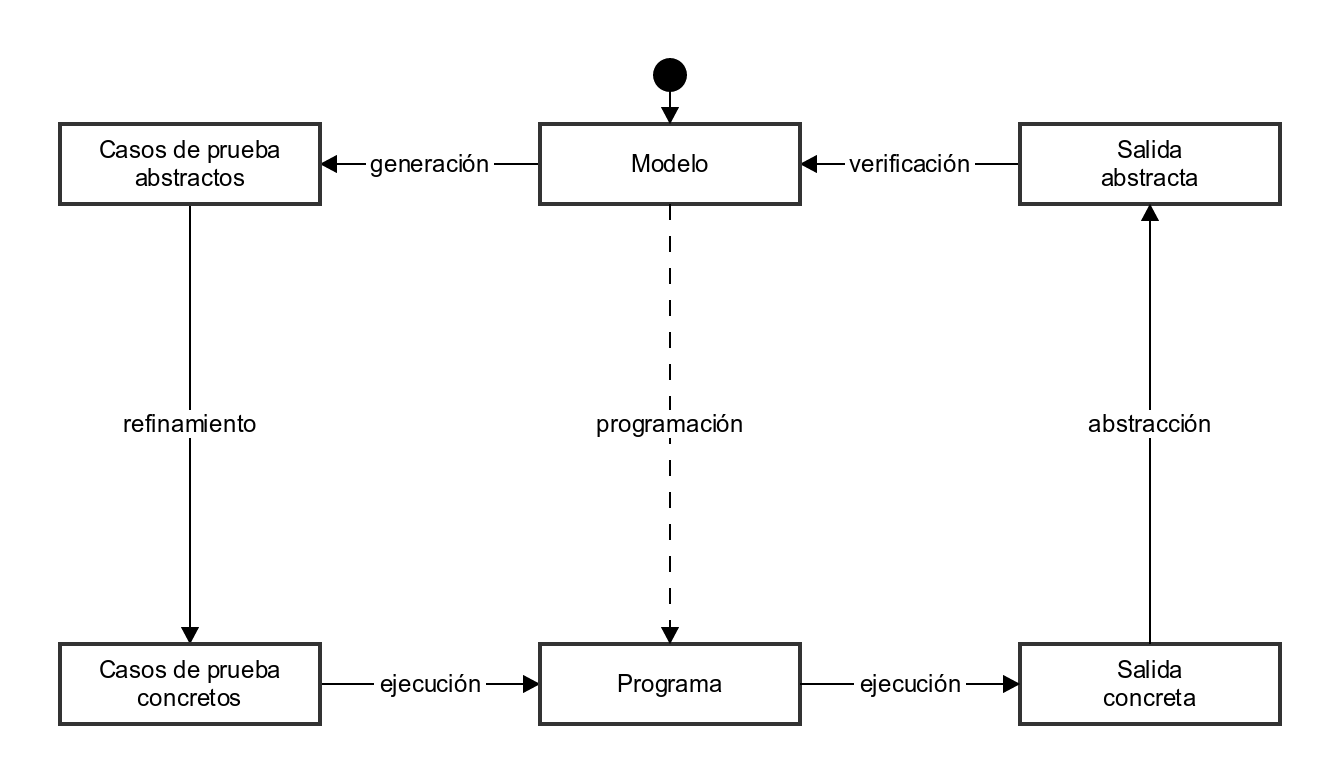
\includegraphics[scale=0.25]{img/proc_mbt.png}
\caption{Proceso de \textit{testing} basado en modelos}
\label{fig:proc_mbt}
\end{center}
\end{figure}


El \textit{Test Template Framework} (TTF) descrito por Stocks y Carrington~\cite{stocks} es un método de MBT que permite efectuar un \textit{testing} muy completo de un sistema del cual se posee una especificación Z~\cite{spivey}, utilizando la misma como entrada y estableciendo cómo generar casos de prueba para testear las distintas operaciones incluidas en el modelo.

A continuación introduciremos brevemente el TTF mediante un ejemplo, asumiendo que el lector se encuentra familiarizado con la notación Z\footnote{Introducción a la notación Z: \url{http://www.fceia.unr.edu.ar/asist/z-a.pdf}}.

\subsection{Ejemplo: \emph{Symbol Table}}
\label{sec:ej-symbolTable}

Una tabla de símbolos es una estructura de datos utilizada por un compilador o intérprete durante el proceso de traducción de un lenguaje de programación donde cada símbolo en el código del programa (variables, constantes, funciones, etc.) se asocia con información como la ubicación, tipo de datos, \textit{scope} de variables, etc. 
En general, en una tabla de símbolos se realizan dos operaciones: inserción y búsqueda; la primera para agregar un símbolo a la tabla y la segunda operación nos permitirá recuperar la información correspondiente a un símbolo ya cargado en la misma.


\bigskip
\noindent
\textbf{Tipos elementales.} Es irrelevante para nuestro modelo especificar en detalle la estructura con la cual representaremos el conjunto de símbolos aceptados por el compilador/interprete, así como la información relativa a los mismos. Para esto, podemos abstraer los conjuntos antes mencionados utilizando los siguientes tipos básicos: 

\begin{zed}
[SYM, VAL] \also
REPORT ::= ok | symbolNotPresent
\end{zed}

El tipo básico \emph{SYM} representará el conjunto de todos los símbolos aceptados por el compilador/interprete, mientras que \emph{VAL} abstraerá el conjunto de toda la información que pudiese estar asociada a un símbolo. Por otro lado, \emph{REPORT} será utilizado para modelar la salida de las operaciones incluidas en la especificación. Una operación podrá ser ejecutada exitosamente o fallar (por ejemplo en caso de realizar una búsqueda de un símbolo que no se encuentre presente en la tabla).
 
\bigskip
\noindent
\textbf{Estado de la tabla.} Es natural pensar que la tabla de símbolos establece una relación funcional entre los símbolos aceptados y la información asociada a cada uno de ellos. Por otro lado, el estado de nuestra tabla está formado únicamente por los símbolos cargados y la información de cada uno. Por lo tanto, podemos modelar el conjuntos de estados de la tabla mediante una única función parcial\footnote{Utilizamos una función parcial ya que no todos los símbolos aceptados por el compilador estarán presentes en la tabla.} de la siguiente manera:

\begin{schema}{ST}
st: SYM \pfun VAL
\end{schema}

\bigskip
\noindent
\textbf{Operaciones.} Como mencionamos anteriormente, dos operaciones se realizarán sobre la tabla de símbolos: inserción y búsqueda.

\bigskip
Comenzaremos por modelar la operación de inserción o actualización. Esta operación modificará el estado de la tabla de símbolos; para esto, será necesario brindarle a la operación el símbolo y la información correspondiente al mismo.

Para actualizar la información de un símbolo en la tabla, simplemente actualizaremos la relación funcional con un par ordenado construido a partir del símbolo y la información dada. 

\begin{schema}{Update}
  \Delta ST \\
  s?: SYM \\
  v?: VAL \\
  rep!: REPORT
  \where
  st' = st \oplus \{s? \mapsto v?\} \\
  rep! = ok
\end{schema}

Por último, deberemos especificar la operación encargada de recuperar la información vinculada a un símbolo. Se trata de una operación relativamente simple que no modifica el estado de la tabla de símbolos. Ésta requerirá de un símbolo a buscar y retornará la información vinculada al mismo. A continuación especificaremos el caso exitoso para esta operación:

\begin{schema}{LookUpOk}
\Xi ST \\
s?: SYM \\
v!: VAL \\
rep!: REPORT
\where
s? \in \dom st \\
v! = st~s? \\
rep! = ok
\end{schema} 

Utilizamos la variable de salida \emph{rep!} para comunicar el éxito o fracaso de la operación, y la variable \emph{v!} para retornar la información solicitada. 

El esquema \emph{LookUpOk} modela solamente el caso en el que el símbolo a buscar se encuentre cargado en la tabla, pero deberemos contemplar también el caso en que se intente buscar un símbolo que no haya sido cargado en la misma. Modelaremos esta situación con el esquema de error \emph{LookUpE}, presentado a continuación:

\begin{schema}{LookUpE}
\Xi ST \\
s?: SYM \\
rep!: REPORT
\where
s? \notin \dom st \\
rep! = symbolNotPresent
\end{schema}

Finalmente, la operación total (que es la que se debe programar) queda definida de la siguiente manera:

\bigskip
$LookUp == LookUpOk \lor LookUpE$

\subsection{\emph{Test Template Framework}}

La propuesta de Stocks y Carrington~\cite{stocks} es utilizar la especificación Z de una operación como fuente de la cual obtener casos de prueba para testear el programa que supuestamente la implementa. La idea se basa en que la especificación del programa contiene todas las alternativas funcionales que el ingeniero consideró imprescindible describir para que el programador implemente el programa correcto. Por lo tanto, para saber si el programa funciona correctamente es necesario probarlo para cada una de estas alternativas funcionales. 

\subsection{Clases y casos de prueba}

Las alternativas funcionales antes mencionadas pueden expresarse como restricciones sobre las variables de entrada y de estado definidas para la especificación. Estas alternativas pueden ser especificadas mediante esquemas Z a los que llamaremos \emph{clases de prueba}. Por ejemplo:

\begin{zed}
   LookUp_{1}^{DNF} == [st: SYM \pfun VAL; s?: SYM  | s? \in \dom st] \\
\end{zed}

\noindent
define una clase de prueba para el esquema \emph{LookUp}, introducido anteriormente, donde $st$ y $s?$ son variables de estado y de entrada respectivamente, y $s? \in \dom st$ es la restricción sobre las mismas. 

Por otro lado, necesitaremos buscar valores específicos, o constantes, para las variables de una \emph{clase de prueba} (que reduzcan su restricción a verdadero) a fin de luego refinarla y poder ejecutar el caso de prueba en el programa que implemente la especificación. Llamaremos \emph{caso de prueba} a la tupla conformada por los valores correspondientes a cada una de las variables involucradas en la clase de prueba que satisfagan la restricción de ésta. Nos bastará con escoger un único \emph{caso de prueba} para cada clase de prueba generada (observemos que en algunos casos, como por ejemplo para la clase de prueba antes presentada, podríamos encontrar infinitos valores posibles para las variables de la clase de prueba que cumplan con la restricción).

Como mencionamos recientemente, los casos de prueba son tuplas conformadas por constantes correspondientes a cada una de las variables involucradas en las clases de prueba correspondientes. Para los tipos dados por el lenguaje, como por ejemplo $\mathbb Z$, las constantes ya se encuentran definidas en el lenguaje, pero esto no ocurre cuando trabajamos con tipos introducidos por el especificador, como $SYM$ y $VAL$ definidos en el ejemplo que venimos estudiando. En estas circunstancias, será necesario definir constantes para estos tipos de datos a fin de poder luego utilizarlas en nuestros casos de prueba. Continuando con el ejemplo, para $SYM$ y $VAL$ podemos definir:

\begin{axdef}
sym_{1}: SYM \\
val_{1}: VAL
\end{axdef}

Ahora que contamos con estas constantes, estamos en condiciones de definir un caso de prueba para la clase de prueba $LookUp_{1}^{DNF}$ de la siguiente manera:

\begin{figure}[H]
\center
$LookUp_{TC}^{1} == [LookUp_{1}^{DNF}  | st = \{sym_{1} \mapsto val_{1} \} \land s? = sym_{1}]$
\end{figure}

Podemos observar en el caso de prueba presentado que hemos asignamos una constante a cada una de las variables del $VIS$ de forma tal que satisfaga la restricción de la clase de prueba en cuestión.

\subsection{Generación de clases de prueba}
\label{sec:tacticas-testing}

En esta sección introduciremos brevemente, por medio de un ejemplo, el proceso del TTF. Continuaremos trabajando sobre el ejemplo introducido anteriormente e intentaremos generar algunos casos de prueba para testear la operación \emph{LookUp}. En particular nos concentraremos en la generación de clases de prueba, que resultarán de vital interés para nuestro trabajo de NLG.

El primer paso del TTF será definir el espacio de entrada (\emph{IS}, por \emph{Input Space}) para la operación. Este será el conjunto definido por todos los posibles valores de entrada y estado de la misma. Por ejemplo, el \emph{IS} para la operación \emph{LookUp} será:

\begin{zed}
  IS == [st: SYM \pfun VAL; s?: SYM]
\end{zed}

En los casos en los que las operaciones son parciales, no tendrá sentido probar el sistema con casos de prueba para los cuales no está definida la operación, es por esto que, a partir del \emph{IS}, el TTF definirá luego el espacio válido de entrada (\emph{VIS}, por \emph{Valid Input Space}). Este será un subconjunto del anterior, formado por los elementos pertenecientes al \emph{IS} que cumplan con la precondición de la operación en cuestión, es decir:

\begin{zed}
  VIS_{Op} == [IS | pre~Op]
\end{zed}

El \emph{VIS} será un subconjunto del \emph{IS} para los cuales tiene sentido testear el programa. Para el caso de \emph{LookUp} será:

\begin{zed}
  VIS_{LookUp} == IS
\end{zed}

\noindent
ya que la operación es total. El \emph{IS} y el \emph{VIS} no coincidirían si la operación \emph{LookUp}, por ejemplo, no se hubiera incluido el esquema de error. En ese caso tendríamos:

\begin{zed}
  IS == [st: SYM \pfun VAL; s?: SYM] \\
  VIS_{LookUpOk} == [IS | s? \in \dom st]
\end{zed}

Luego de determinar el \emph{VIS}, el TTF propone dividir el mismo, de modo tal que cada una de estas particiones represente una alternativa funcional distinta de la operación a testear. Estas particiones serán las \emph{clases de prueba}, introducidas anteriormente. Para dividir el $VIS$ a fin de dar con éstas, será necesario aplicar alguna estrategia o \emph{táctica de testing} que establezca la forma en la cual puede ser particionado el $VIS$. Luego, será posible aplicar nuevas tácticas sobre estas particiones generadas a fin de dividir nuevamente las mismas, obteniendo como resultado nuevas clases de prueba; este proceso se podrá repetir hasta que el ingeniero de \textit{testing} considere que todas las alternativas funcionales importantes de la operación están representadas (cada una de estas alternativas corresponderá a una única clase de prueba). El último paso del proceso será la selección de al menos un \emph{caso de prueba} para cada clase de prueba, que, como vimos anteriormente, consistirá en buscar valores para las variables de la misma que reduzcan su restricción a verdadero. 

A continuación, mostraremos la aplicación de algunas tácticas de \textit{testing} sobre la operación \emph{LookUp}. En primer lugar aplicaremos Forma Normal Disyuntiva (DNF del inglés \emph{``Disjunctive Normal Form''}) y luego aplicaremos la táctica de Partición Estándar (SP del inglés \emph{``Standard Partition''}) a la expresión: ``$s? \in \dom st$''.

\bigskip
\noindent
\textbf{Forma Normal Disyuntiva.} Suele ser la primer táctica que se aplica. Esta expresará la operación como una disyunción de esquemas en los cuales únicamente habrá conjunciones de literales o de negaciones de literales y luego dividirá el \emph{VIS} con las pre-condiciones de cada esquema. 

Continuando con el ejemplo, \emph{LookUp} ya es una disyunción y cada uno de los esquemas que la forman se encuentra en DNF (del inglés \emph{Disjunctive Normal Form}). Por lo tanto, solo deberemos dividir el \emph{VIS} con la precondición de cada uno de ellos, de la siguiente forma:

\begin{zed}
  LookUp_{1}^{DNF} == [VIS_{LookUp} | s? \in \dom st] \\
  LookUp_{2}^{DNF} == [VIS_{LookUp} | s? \notin \dom st]
\end{zed}

De esta forma obtenemos una partición del \emph{VIS}\footnote{Esto no se cumple en todos los casos, podrían ``solaparse'' las particiones obtenidas, pero de cualquier forma lograríamos un cubrimiento funcional básico.}. Además, observemos que si tomamos un caso de prueba para cada una de las clases obtenidas estaríamos probando el sistema en las siguientes situaciones:

\begin{enumerate}
\item Intentar buscar un símbolo cargado en la tabla de símbolos.
\item Intentar buscar un símbolo que no fue cargado previamente en la tabla de símbolos.
\end{enumerate}

\bigskip
\noindent
\textbf{Partición Estándar.} Esta táctica trata con los operadores matemáticos de una operación. Una partición estándar es una partición del dominio del operador en conjuntos llamados \emph{sub-dominios}. En la figura~\ref{ej:partition_in} podemos ver la partición estándar utilizada por \emph{Fastest} para el operador $\in$.

\begin{figure}[H]
\begin{framed}
  \begin{enumerate}
    \item $A = \{a\}$
    \item $A \neq \{a\}, a \in A$
  \end{enumerate}
  \end{framed}
  \caption{Partición estándar para $a \protect\in A$}
  \label{ej:partition_in}
\end{figure}

Para aplicar esta táctica primero hay que seleccionar un operador de un predicado incluido en el esquema de la operación a testear.

Siguiendo con el ejemplo anterior, aplicaremos la técnica de partición estándar a la clase de prueba $LookUp_{1}^{DNF}$. En primer lugar, deberemos seleccionar una aparición de un operador en el esquema de la operación \emph{LookUp}. 
Nosotros elegiremos el operador $\in$ de la expresión ``$s? \in \dom st$''.


El siguiente paso será reemplazar los parámetros formales que aparecen en la descripción de la partición por las expresiones usadas en la especificación.  En particular, para nuestro ejemplo, deberemos reemplazar los parámetros de las expresiones que aparecen en la figura~\ref{ej:partition_in} con las expresiones ``$s?$'' y ``$\dom st$''. Finalmente, a partir de la clase de prueba sobre la cual se quiere aplicar la táctica, tendremos que generar las nuevas particiones para cada uno de los sub-dominios definidos en la partición estándar. En consecuencia, obtendremos las siguientes clases:


\begin{zed}
  LookUp_{1}^{SP} == [LookUp_{1}^{DNF} | \dom st = \{s?\}] \\
  LookUp_{2}^{SP} == [LookUp_{1}^{DNF} | \dom st \neq \{s?\} \land s? \in \dom st] \\
\end{zed}

Luego podríamos continuar aplicando nuevas tácticas y particionando aún más el \emph{VIS}. En este caso se trata de una operación relativamente sencilla y consideramos que todas las alternativas funcionales importantes se encuentran representadas mediante las clases de prueba obtenidas.

\subsection{Fastest}
\label{sec:fastest}

\emph{Fastest}\footnote{\url{http://www.fceia.unr.edu.ar/~mcristia/fastest-1.6.tar.gz}} es una herramienta que implementa la teoría del TTF desarrollada en primer instancia por Maximiliano Cristiá y Pablo Rodriguez Monetti~\cite{fastest1}. El desarrollo de la misma fue impulsado para intentar automatizar, lo máximo posible, el proceso de \textit{testing} funcional basado en especificaciones Z. \emph{Fastest} se encuentra implementado mayormente en lenguaje Java y hace uso de las librerías del \textit{framework} CZT\footnote{\url{http://czt.sourceforge.net/}} (\emph{Community Z Tools}) para contar con utilidades relacionadas al lenguaje de especificación Z. 

A continuación, en la figura \ref{ej:comandos_fastest}, ilustraremos el funcionamiento de \emph{Fastest} mostrando los comandos necesarios para generar las clases de prueba introducidas anteriormente en esta sección.


\begin{figure}[H]
\begin{Verbatim}[frame=single,fontsize=\scriptsize]
Fastest version 1.6, (C) 2013, Maximiliano Cristiá
Loading pruning rewrite rules...
Loading pruning theorems...
Fastest> loadspec symbolTable.tex
Loading specification..
Specification loaded.
Fastest> selop LookUp
Fastest> genalltt 
Generating test tree for 'LookUp' operation.
Fastest> addtactic LookUp_DNF_1 SP \in s? \in \dom st
Fastest> genalltt                                    
Fastest> showsch -tcl -u 2

\begin{schema}{LookUp\_ DNF\_ 1}\\
 st : SYM \pfun VAL \\
 s? : SYM 
\where
 s? \in \dom st
\end{schema}

\begin{schema}{LookUp\_ SP\_ 1}\\
 st : SYM \pfun VAL \\
 s? : SYM 
\where
 s? \in \dom st \\
 \dom st = \{ s? \}
\end{schema}

\begin{schema}{LookUp\_ SP\_ 2}\\
 st : SYM \pfun VAL \\
 s? : SYM 
\where
 s? \in \dom st \\
 \dom st \neq \{ s? \} \\
 s? \in \dom st
\end{schema}

\begin{schema}{LookUp\_ DNF\_ 2}\\
 st : SYM \pfun VAL \\
 s? : SYM 
\where
 s? \notin \dom st
\end{schema}
\end{Verbatim}
\caption{Comandos para generación de clases de prueba en \emph{Fastest}}
\label{ej:comandos_fastest}
\end{figure}

Como se podemos observar en la figura \ref{ej:comandos_fastest}, en primera instancia cargamos la especificación en \emph{Fastest} mediante el comando \texttt{loadspec}. \emph{Fastest} realiza algunas verificaciones sintácticas y de tipado sobre la especificación, para luego informar por pantalla en caso de encontrar algún error en la misma. El comando \texttt{selop} selecciona un esquema con el cual trabajar (para el ejemplo anterior seleccionamos sólo uno, pero es posible seleccionar más esquemas). Luego, \texttt{genaltt} es utilizado, en este caso, para aplicar la táctica de DNF (\emph{Disjunctive Normal Form}); esta táctica es aplicada por defecto la primera vez que es ejecutado el comando. El comando \texttt{addtactic} añadirá una nueva táctica de partición, pero no ejecutará la misma. Será necesario volver a ejecutar \texttt{genaltt} para realizar la partición en base a la táctica ingresada. Finalmente, mostramos por pantalla todas las clases de prueba generadas por \emph{Fastest} utilizando el comando \texttt{showsch} (el parámetro \texttt{-tcl} fue utilizado para indicar que sólo queremos imprimir clases de prueba, mientras que \texttt{-u} fue utilizado para indicarle a \emph{Fastest} que queremos expandir las definiciones de las mismas).

Observemos que \emph{Fastest} utiliza una notación levemente diferente, pero equivalente, a la introducida en este capítulo para nombrar las clases y casos de prueba. En lo que queda de este trabajo, seguiremos estilo propuesto por \emph{Fastest} cuando hagamos referencia a clases y casos de prueba generados por medio de esta herramienta.

En lo que respecta a la generación de lenguaje natural, \emph{Fastest} fue utilizado en el pasado para testear el software a bordo de un satélite~\cite{satelite} y posteriormente se utilizaron técnicas de generación de lenguaje natural basada en \textit{templates} para traducir los casos de prueba obtenidos \cite{cristia_pluss}. La situación propuesta en el trabajo recién mencionado fue una solución ad-hoc, dependiente del dominio de aplicación y de la cantidad de operaciones.


Como mencionamos anteriormente, uno de los objetivos de este trabajo será el de extender la implementación de \emph{Fastest} para permitir al usuario generar descripciones, independientes del dominio de aplicación y de la cantidad de operaciones de las clases de prueba generadas con la herramienta.
El sistema de NLG a desarrollar en este trabajo será íntegramente implementado en Java e integrado como una extensión de \emph{Fastest} (trabajando para esto con la versión 1.6 de la herramienta). En el capítulo \ref{cap:implementacion} veremos algunos de los detalles más relevantes de esta implementación.

\section{Designaciones}
\label{cap:designaciones}

Un modelo formal, como una especificación Z en este caso, es una abstracción de la realidad. Sin embargo, se realiza una especificación para escribir un programa que finalmente es usado en el mundo real. En consecuencia, existe una relación entre el modelo y la realidad.
Normalmente en estos casos, cuando especificamos un sistema formalmente, es una práctica común incluir asociaciones entre elementos de la especificación (operaciones, esquemas de estado, variables, constantes, etc.) y elementos que refieran al dominio de aplicación. Estas asociaciones son llamadas \emph{designaciones}~\cite{jackson}.
Sin esta documentación el modelo sería nada más que una teoría axiomática más sin conexión con la realidad. 

Para documentar las designaciones usaremos la sintaxis propuesta por Jackson~\cite{jackson}:

\begin{figure}[H]
  \centering
  \emph{texto informal} $\approx$ \textbf{término\_formal}
\end{figure}

El símbolo $\approx$ demarca la frontera entre el mundo real (a la izquierda) y el mundo formal o lógico (a la derecha). Del lado derecho estará el término formal a designar, este será un elemento de la especificación, mientras que del otro lado tendremos texto informal en lenguaje natural que permitirá reconocer el fenómeno designado.

Continuando con el ejemplo de la tabla de símbolos (sección ~\ref{sec:ej-symbolTable}), podríamos contar (entre otras) con las siguientes designaciones:

\begin{figure}[H]
  \begin{align*} 
    &\text{Símbolo a buscar} && \approx &&&s? \\
    &\text{Información asociada a $x$} && \approx &&&st~x
  \end{align*}
  \caption{Algunas designaciones para \emph{SymbolTable}}
  \label{fig:ej_designacion}
\end{figure}


Para Jackson, las designaciones sirven en primera instancia cuando se empieza a escribir la especificación para diferenciar un fenómeno en particular y darle un nombre. Luego, le será de utilidad al programador a la hora de leer la especificación. Jackson propone construir un \emph{``puente angosto''} entre la especificación y los elementos del dominio, escribiendo la menor cantidad de designaciones posibles y definiendo otros términos en base a las anteriores.


La función que cumplirán las designaciones en éste trabajo difiere un poco de la propuesta por Jackson. Para nosotros las designaciones resultarán la principal fuente de conocimiento para nuestro sistema de NLG. Y serán fundamentales para que éste pueda generar descripciones independientes del dominio de aplicación.

Veamos, por ejemplo, las siguientes expresiones pertenecientes a dos clases de prueba de dos especificaciones distintas:

\begin{figure}[H]
\begin{enumerate}
\item $\dom st = \{ s? \}$
\item $\dom cajas = \{ num? \}$
\end{enumerate}
\end{figure}

La primera expresión pertenece a una clase de prueba generada para la operación \emph{LookUp}, la segunda es parte de una clase de prueba generada para una operación perteneciente a la especificación de un sistema bancario. Estas expresiones resultan equivalentes (de hecho, hasta podríamos haber usado los mismos nombres de variables para ambas especificaciones); será gracias a las designaciones que podremos otorgarles una descripción en lenguaje natural (acorde al dominio de aplicación de cada especificación) a cada una de estas expresiones. En particular, para estas, las descripciones podrían ser las siguientes:

\begin{figure}[H]
\begin{enumerate}
\item \emph{``El símbolo a buscar es el único elemento de los símbolos cargados en la tabla.''}
\item \emph{``El número de cuenta del nuevo cliente es el único elemento de los números de cuenta cargados en el banco.''}
\end{enumerate}
\end{figure}

Los sistemas de generación de lenguaje natural generalmente utilizan un diccionario de palabras o frases, las cuales se utilizan para referirse a fenómenos del dominio. En nuestro caso, el dominio de aplicación dependerá de la especificación en cuestión y de lo que se modele con la misma, por lo tanto, las designaciones resultarán nuestra única fuente de textos dependientes del dominio y es por eso que serán un elemento fundamental para nuestro sistema de NLG.

Por otro lado, en algunas situaciones, contar con una mayor cantidad de designaciones nos permitirá generar mejores descripciones. Designaciones que podrían resultar redundantes para una persona que lea la especificación podrían, por ejemplo, permitirle a nuestro sistema de NLG generar textos más naturales. En el apéndice \ref{ape:designaciones} podemos encontrar una pequeña guía sobre qué designar a fin de proveerle la información necesaria a nuestro sistema de NLG para que pueda producir textos más fluidos y naturales.

Por último, cabe mencionar, que es posible que aparezcan parámetros (pertenecientes al término formal) también del lado izquierdo de la designación, como es el caso de la segunda designación presente en la figura~\ref{fig:ej_designacion}. Llamaremos \emph{designaciones parametrizadas} a este tipo de designaciones, y marcaremos esta diferencia ya que deberemos darle un tratamiento especial a fin de utilizar el texto de estas designaciones en nuestro sistema de NLG. En la sección~\ref{sec:verbalizacion_designaciones} desarrollaremos más en detalle esta particularidad. 


\section{Resumen del capítulo}
En este capítulo introdujimos conceptos fundamentales para el desarrollo de este trabajo. Presentamos el \textit{test template framework}, definimos las nociones de clase y caso de prueba con las que trabajaremos a lo largo de todo el trabajo. Finalmente profundizamos sobre el rol que cumplirán las designaciones en este trabajo, resultando fundamentales para la generación de descripciones independientes del dominio de aplicación. En el próximo capítulo introduciremos las tareas que deberán ser llevadas a cabo por nuestro sistema de NLG para generar descripciones para las clases de prueba generadas por Fastest.
\chapter{Generación de lenguaje natural.}
\label{cap:nlg_intro}
La generación de lenguaje natural (NLG) es un una rama de la lingüística computacional y la inteligencia artificial encargada de estudiar la construcción de sistemas computacionales capaces de producir texto en castellano o cualquier otra lengua humana a partir de algún tipo de representación no-lingüística de la información a comunicar. Estos sistema combinan conocimientos tanto del lenguaje en cuestión cómo del dominio de aplicación para producir automáticamente documentos, reportes, mensajes o cualquier otro tipo de textos.

Dentro de la comunidad desarrolladora e investigadora de la NLG hay un cierto consenso sobre la funcionalidad lingüística general de un sistema de NLG.
En este trabajo se optó por seguir la metodología más comúnmente aceptada, propuesta por Reiter y Dale~\cite{reiter_dale}.
A continuación describiremos brevemente los aspectos mas importantes de esta metodología y en capítulos posteriores desarrollaremos más en profundidad en los puntos mas relevantes para nuestro trabajo.

\section{Análisis de requerimientos}
El primer paso en la construcción de cualquier sistema de software, incluyendo los sistemas de generación de lenguaje natural, será el de realizar un análisis de requerimientos y a partir de ahí generar una especificación inicial del sistema. 

Para el análisis de requerimientos, Reiter y Dale proponen realizar un \emph{corpus} de textos de ejemplo y a partir de ellos obtener una especificación para el sistema a desarrollar. Estos ejemplos estarán compuestos por una colección de datos de entrada del sistema con sus respectivas salidas (texto en lenguaje natural). Estos deberán estar redactados por un humano experto y deberían caracterizar todas las salidas posibles que se espera que el sistema genere.

En el capítulo~\ref{cap:corpus} profundizaremos más sobre este tema, describiremos y analizaremos el \emph{corpus de descripciones} utilizado para este trabajo.

\section{Tareas de la generación de lenguaje natural}

Dentro de la comunidad desarrolladora e investigadora de la generación de lenguaje natural, hay cierto consenso sobre las tareas que deben llevarse a cabo para, a partir de los datos de entrada, generar texto final en lenguaje natural. 

La más comúnmente aceptada es la clasificación de Reiter y Dale que distingue las siguientes siete tareas que deben ser realizadas a lo largo de todo el proceso: 

\bigskip
\noindent
\textbf{Determinación del contenido:} es el proceso de determinar que información debe ser comunicada en el texto final; será el encargado de que el mismo contenga toda la información requerida por el usuario. Generalmente involucra una o más tareas de selección, resumen y razonamiento con los datos de entrada.

\bigskip
\noindent
\textbf{Estructuración del documento:} es el proceso de imponer un orden y estructura sobre los textos generados a fin de que la información del documento final se encuentre estructurada de forma entendible y fácil de leer.

\bigskip
\noindent
\textbf{Lexicalización:} es el proceso de decidir que palabras y frases especificas usar para expresar los distintos conceptos y relaciones del dominio. En esta etapa se deberá establecer como se expresa un significado conceptual concreto, descrito en términos del modelo del dominio, usando elementos léxicos (sustantivos, verbos, adjetivos, etc).

\bigskip
\noindent
\textbf{Generación de expresiones de referencia:} es la tarea de elegir que expresiones usar para identificar entidades del dominio de aplicación. Podríamos querer referirnos a una determinada entidad de distintas formas. Por ejemplo: podríamos querer referirnos al mes en curso como, ``febrero'', ``este mes'', ``este'', etc.

\bigskip
\noindent
\textbf{Agregación:} se encarga de combinar dos o mas elementos informativos con el fin de conseguir un texto más fluido y legible. La agregación decide que elementos se pueden agrupar para generar oraciones mas complejas sin modificar el significado de las mismas. Por Ejemplo, dos frases de una descripción para una clase de prueba de un scheduler se podrían expresar como:
\emph{``El proceso a borrar se encuentra en la tabla de procesos. El estado del proceso a borrar es waiting.''} o \emph{``El proceso a borrar se encuentra en la tabla de procesos y el estado del mismo es waiting.''}

\bigskip
\noindent
\textbf{Realización lingüística:} es el proceso de aplicar reglas gramaticales (a estructuras generadas por las etapas anteriores) con el fin de producir un texto que sea sintáctica, morfológica y ortográficamente correcto.

\bigskip
\noindent
\textbf{Realización de la estructura:} esta tarea se encarga de convertir estructuras abstractas como párrafos y secciones (generadas por etapas anteriores) en texto comprensible por el componente de presentación del documento. Por ejemplo, la salida del sistema de NLG podría ser código LaTeX para luego ser post-procesado, en este caso sería esta etapa la encargada de agregar delimitadores y comandos de LaTeX para generar el documento. 

\section{Arquitectura para la NLG.}
Existen muchas maneras de construir un sistema que realice las tareas antes mencionadas. Una forma podría ser construir un único módulo encargado de llevar a cabo todas las tareas en simultaneo. En el otro extremo, podríamos tener un módulo separado para cada tarea y conectarlos mediante un \emph{pipeline}. En este caso, el sistema primero se encargaría de la determinación de contenido, luego la estructuración del documento, y así sucesivamente. La desventaja de este último modelo es que asume que las tareas deben ser realizadas en un único orden y que las funcionalidades de las mismas no se solapan.

En este trabajo utilizaremos la arquitectura mas comúnmente utilizada para sistemas de NLG. Esta consiste de tres módulos conectados mediante un \emph{pipeline}. La misma se encuentra en el medio de los dos extremos antes mencionados.

\begin{figure}[h]
  	\centering
	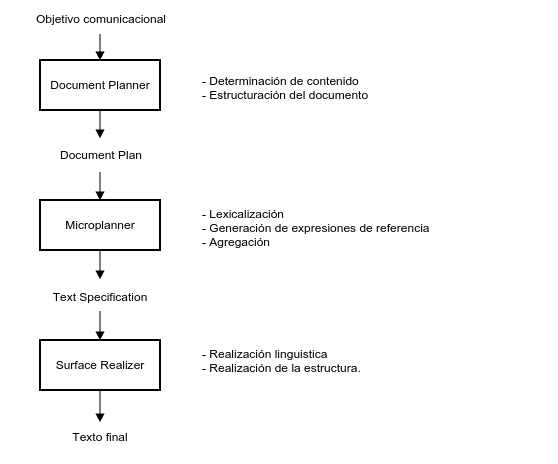
\includegraphics{img/arquitectura.png}
	\caption{Arquitectura típica sistema NLG.}
  	\label{fig:png_arquitectura}
\end{figure}

El primer módulo de nuestro sistema será el \emph{document planner}, encargado de realizar las tareas de determinación de contenido y estructuración del documento. Veremos en el capítulo~\ref{cap:document_planning} que estas tareas se encuentran sumamente relacionadas y son realizadas en simultaneo. La salida de esta etapa y entrada del \emph{microplanner} será un \emph{document plan}, este será una abstracción del documento final que contendrá los elementos informativos que se desea comunicar.

El segundo módulo será el encargado de realizar las tareas de lexicalización, generación de expresiones de referencia y agregación. La función del mismo será la de trabajar el document plan generando una especificación mas refinada del texto final, una \emph{text specification}. El \emph{microplanner} será el responsable de transformar los elementos informativos incluidos en el document plan en una especificación mas concreta de una oración. En el capítulo~\ref{cap:microplanning} desarrollaremos mas en profundidad el funcionamiento del microplanner.

Finalmente el \emph{surface realiser} tomará como entrada el text specification generado por la etapa anterior y será el encargado de producir el texto final. Este módulo deberá llevar a cabo las tareas de realización lingüística y de superficie ates mencionadas.
\include{sec/alcance}
\chapter{Análisis de requerimientos}
\label{cap:corpus}

El primer paso en la construcción de cualquier sistema de software, incluyendo los sistemas de generación de lenguaje natural, es realizar un análisis de requerimientos y a partir de estos generar una especificación inicial para el sistema. Para el análisis de requerimientos, se seguirá el enfoque sugerido por Reiter y Dale~\cite{reiter_dale} en el cual se propone realizar un corpus de textos de ejemplo y a partir de ellos obtener los requerimientos para el trabajo.

\section{Corpus de descripciones}                 

Según la definición de la RAE~\cite{dicrae}, un corpus es un \emph{``conjunto lo más extenso y ordenado posible de datos o textos científicos, literarios, etc., que pueden servir de base a una investigación''}. En particular, el corpus utilizado para la construcción de un sistema de NLG estará formado por un conjunto de ejemplos de datos de entrada junto a la correspondiente salida (texto en lenguaje natural) para cada uno de estos. En nuestro caso, la entrada será un grupo de clases de prueba (en lenguaje Z) junto a las designaciones correspondientes a la especificación testeada, mientras que la salida estará formada por descripciones en lenguaje natural de las clases de prueba antes mencionadas. En lo posible, el corpus de textos deberá cubrir todo el rango de textos que esperan ser producidos por el sistema de NLG; éste debería cubrir los casos más frecuentes, así como los casos más inusuales que pudieran ocurrir.

%~\footnote{Una vez recolectada una colección inicial de textos de ejemplo, es posible que sea necesario aplicar algunas modificaciones sobre ésta. Esto se puede deber a que algunos de los textos recolectados resulten técnicamente implosibles de generar y sea necesarios removerlos del corpus, que existan diferentes variantes correspondientes a la misma entrada de texto y requiramos resolver posibles conflictos, textos que puedan ser mejorados y puedan ser modificados, etc. Llamaremos corpus objetivo al resultado de aplicar al corpus inicial todas las modificaciones antes mencionadas (de ser necesarias).}
Siguiendo la metodología propuesta por Reiter y Dale, para construir el corpus que se utilizará a lo largo de todo el trabajo se deberá elaborar, en primera instancia, un \emph{corpus inicial} y luego, de ser necesario, se deberá trabajar el mismo a fin de confeccionar un \emph{corpus objetivo} que será con el que finalmente se trabajará. Para construir un \emph{corpus inicial} se debe recolectar un conjunto lo suficientemente amplio de ejemplos que debería ser representativo de la variedad de textos que se desea generar. Luego una persona capacitada (en nuestro caso alguien capaz de leer esquemas Z y con un alto conocimiento del dominio de aplicación) deberá describir en lenguaje natural los ejemplos antes mencionados. Esta colección de ejemplos y descripciones de los mismos constituirá nuestro \emph{corpus inicial}. Es posible que esta recopilación requiera algunas modificaciones, por ejemplo: podría ocurrir que alguno de los textos resulten técnicamente imposibles de generar y sea necesarios removerlos del corpus, también podrían existir diferentes variantes correspondientes a la misma entrada de texto y deberíamos resolver los posibles conflictos, etc. Llamaremos, finalmente, \emph{corpus objetivo} al resultado de aplicar las modificaciones necesarias al \emph{corpus inicial}. Este \emph{corpus objetivo} es el que se utilizará para sustentar muchas de las decisiones que se tomarán a lo largo de este trabajo. Además, podría ser de utilidad\footnote{Esto no está contemplado dentro del alcance de este trabajo, pero como veremos en el capítulo \ref{cap:conclusion}, podría ser tenido en cuenta en trabajos futuros.} para realizar una evaluación de nuestro sistema una vez desarrollado, comparando los textos generados por la implementación realizada con las descripciones del corpus realizadas por la persona especializada.

En el apéndice~\ref{ape:corpus} podemos encontrar los textos incluidos en el corpus utilizado para este trabajo. Para elaborar el mismo, se ha recolectado una colección de clases de prueba generadas con \emph{Fastest} a partir de distintas especificaciones y luego se escribió manualmente cada una de las descripciones para las mismas. En este proceso, se intentó abarcar todo el rango de textos que se espera que nuestro sistema sea capaz de producir, para esto, se ha tenido en cuenta incluir una gran variedad de clases de pruebas de modo que cubran todas las expresiones u operadores de Z contemplados dentro del alcance de este trabajo, considerando también las posibles combinaciones de estas expresiones. Se trabajó también con especificaciones sobre distintos dominios de aplicación a fin de lograr un corpus que sea de utilidad para dar con una solución independiente del dominio de aplicación. En total se han incluido clases de prueba generadas con \emph{Fastest} para 5 especificaciones distintas; del total se escogieron las más significativas para describir en lenguaje natural y se ignoraron aquellas que contenían algún operador no considerado dentro del alcance de este trabajo.


En la figura~\ref{fig:ej_corpus} podemos observar uno de los ejemplos incluidos en el corpus de descripciones utilizado para este trabajo. En este caso la clase de prueba \emph{LookUp\_SP\_1} (generada a partir de la especificación introducida previamente) y las designaciones correspondientes a la especificación en cuestión serán la entrada del sistema de NLG\footnote{Estrictamente hablando, todas las designaciones de la especificación deberían formar parte de la entrada del sistema de NLG. En este caso, se incluyeron sólo las designaciones relevantes a fin de simplificar el ejemplo.}, teniendo como salida la descripción en lenguaje natural presente en el ejemplo.

\begin{figure}[H]
\begin{itemize}
\item \emph{Clase de prueba para operación LookUp}\\
\begin{schema}{LookUp\_ SP\_ 1}\\
 st : SYM \pfun VAL \\
 s? : SYM 
\where
 s? \in \dom st \\
 \dom st = \{ s? \}
\end{schema}

\item \emph{Designaciones SymbolTable}\\

\begin{itemize}[label={--}]
  \item símbolo a buscar $\approx s?$
  \item símbolos cargados en la tabla $\approx \dom st$
\end{itemize}

\bigskip
\item \emph{Descripción en lenguaje natural para LookUp\_SP\_1}\\

\begin{tcolorbox}[colback=gray!5!white,colframe=gray!50!black,
  colbacktitle=gray!75!black,title=LookUp\_SP\_1]
  Se busca un símbolo en la tabla, cuando:
     \begin{itemize}
  	    \item[--]{El símbolo a buscar pertenece a los símbolos cargados en la tabla.}
        \item[--]{El símbolo a buscar es el único elemento de los símbolos cargados en la tabla.} 
     \end{itemize}
\end{tcolorbox}

\end{itemize}
\caption{Corpus de textos}
\label{fig:ej_corpus}
\end{figure}

\section{Análisis del corpus}
\label{sec:corpus_analisis}

En lo que queda de este capítulo nos encargaremos de analizar los ejemplos presentes en el corpus a fin de extraer los requerimientos para nuestro sistema. Este estudio nos ayudará a sustentar muchas las decisiones que se tomarán al realizar el diseño de nuestro sistema de NLG. 

Comenzaremos analizando las clases de prueba generadas por \emph{Fastest} y la correlación entre la estructura de las mismas y la estructura de las descripciones en lenguaje natural. Luego estudiaremos la verbalización de las expresiones Z presentes en las clases de prueba, analizaremos el rol de las designaciones y se dará un conjunto de reglas para describir estas expresiones. Por último se contemplarán cuestiones gramaticales que se deberán tener en cuenta para la realización del sistema.

\section{Estructura de las descripciones}
\label{sec:corpus_descripciones}
Podemos notar que las clases de prueba generadas por \emph{Fastest} se encuentran formadas siempre por conjunciones de predicados atómicos y que a cada uno de estos le corresponde exactamente una oración en lenguaje natural dentro del texto final. Además, estas oraciones dependen exclusivamente del predicado que describen, es decir, éstas no contienen información sobre otros predicados ni hacen referencia a otras frases generadas. En la figura~\ref{fig:ej_test_desc} podemos evidenciar esta correspondencia.

\begin{figure}[H]
\centering
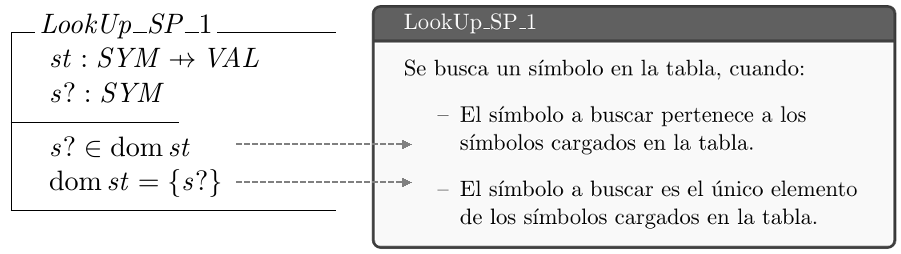
\includegraphics[scale=0.4]{img/ej_test_desc.png}
\caption{Estructura descripciones}
\label{fig:ej_test_desc}
\end{figure}

Además, podemos observar del corpus (apéndice \ref{ape:corpus}) que todas las descripciones de las clases de prueba poseen la misma estructura. En todas se comienza por el nombre de la clase de prueba, seguido por un pequeño detalle de la operación a testear y luego una lista de oraciones encargadas de describir cada uno de los predicados presentes en el cuerpo de la clase de prueba. Conocer la estructura del texto a generar nos será de utilidad para la elaboración del \emph{document plan} (capítulo ~\ref{cap:document_planning}).

\section{Verbalización de expresiones Z}
\label{sec:corpus_verbalizacion}

La tarea de describir un esquema Z correspondiente a una clase de prueba, se puede reducir básicamente a \emph{verbalizar} individualmente cada uno de los predicados atómicos que constituyen el cuerpo del esquema Z. Esta \emph{verbalización} de predicados Z será el desafío principal de este trabajo. Definir con precisión los detalles de ésta será de vital importancia para el desarrollo de las etapas de \emph{microplanning} y \textit{surface realization} de nuestro sistema de NLG (capítulo~\ref{cap:microplanning} y \ref{cap:realization}). En esta sección nos concentraremos especialmente en analizar y especificar la tarea de verbalización.

Podemos notar dos aspectos fundamentales sobre la \emph{verbalización} de expresiones Z. En primer lugar, podemos ver que hay textos que se repiten (con pequeñas variantes, que analizaremos posteriormente) independientemente del dominio de aplicación y que estos surgen a raíz de los operadores de Z presentes en los predicados que se describen. Por otro lado, podemos observar el rol fundamental de las designaciones que posibilitan la introducción de texto dependiente del dominio de aplicación en las descripciones. Consideremos, por ejemplo, las siguientes dos expresiones y sus respectivas descripciones en lenguaje natural, una pertenece al ejemplo de la figura~\ref{fig:ej_corpus} y la otra describe un predicado que forma parte de una clase de prueba para la especificación de un sistema bancario:

\bigskip
\begin{enumerate}
	\item $s? \in \dom st$ $\rightarrow$ \emph{``El símbolo a buscar \textbf{pertenece a}  a los símbolos cargados en la tabla.''}
	\item $s? \in \dom st$ $\rightarrow$ \emph{``El número de cuenta del nuevo cliente \textbf{pertenece a} a los números de cuenta cargados en el banco.''}
\end{enumerate}

\bigskip
Como vemos, el texto \emph{``\textbf{pertenece a}''} aparece en ambas descripciones como resultado de verbalizar el operador $\in$, diferenciándose ambas descripciones en el texto que antecede y sucede al mismo. Por otro lado, estos últimos, bien podrían ser las verbalizaciones de las expresiones que se encuentran a la derecha e izquierda del operador $\in$, respectivamente, por lo que podríamos pensar en una verbalización recursiva sobre la estructura de las expresiones Z. Es posible encontrar estos tipos de patrones en todas las descripciones presentes en el corpus. Esto resulta un buen punto de partida para intentar especificar nuestra tarea de verbalización. En un primer intento, entonces, se definirá la tarea de verbalización en base a los operadores que la componen. Especificaremos esta tarea mediante una función que tomará como entrada una expresión Z y devolverá una descripción en lenguaje natural para la misma. Ésta será recursiva sobre la estructura de las expresiones Z y tendrá tantos casos en su definición como operadores contemplados dentro del alcance de este trabajo (además de las posibles combinaciones de los mismos que puedan resultar de interés y requieran un tratamiento particular). En base al ejemplo anterior, podríamos proponer la siguiente definición para verbalizar el operador $\in$\footnote{Supondremos que el operador $+$ se encargará de realizar una concatenación de \textit{strings} agregando un espacio entre las mismas.}$^{,}$\footnote{El nombre de la función se encuentra primado intencionalmente. Más adelante se presentará la definición final para la función de verbalización que hará uso de \texttt{verb'} como función auxiliar.} :

{
\begin{figure}[H]
\center
$\texttt{verb'} (x \in y) = \texttt{verb}(x) + \text{\emph{``pertenece a''}} + \texttt{verb}(y)$
\end{figure}
}

Como se mencionó anteriormente, para verbalizar términos compuestos se necesitará verbalizar recursivamente las partes que componen a los mismos. En el ejemplo anterior se necesitaría conocer las verbalizaciones de las expresiones $x$ e $y$ para poder obtener una verbalización para $x \in y$.

Retomando el ejemplo de la figura~\ref{fig:ej_corpus}, nos concentraremos en verbalizar la primera expresión de la clase de prueba:

\begin{figure}[H]
\center
$s? \in \dom st$
\end{figure}

En este caso, según la verbalización propuesta anteriormente, podríamos verbalizar la expresión como:

\begin{figure}[H]
\center
$\texttt{verb'} (s? \in \dom st) \rightarrow \texttt{verb}(s?) + \text{\emph{``pertenece a''}} + \texttt{verb}(\dom st)$
\end{figure}

Teniendo que verbalizar $s?$ y $\dom st$. En este caso, ambas expresiones se encuentran designadas, lo que sería de gran ayuda para nuestra tarea de verbalización ya que en estas situaciones podremos construir la descripción en base al texto presente en la designación y sin intentar verbalizar la expresión en base al término Z que la compone. En el ejemplo anterior, no deberíamos intentar verbalizar $\dom st$ como:

\begin{figure}[H]
\center
$\texttt{verb'}(\dom st) \rightarrow \text{\emph{``el dominio''}} + \texttt{verb}(st)$
\end{figure}

\noindent
de hacerlo, estaríamos perdiendo información valiosa para nuestras descripciones contenida en las designaciones ya que las designaciones son nuestra única forma de introducir texto referente al dominio de aplicación en las descripciones. 

En general, para verbalizar una expresión designada, deberemos utilizar el texto presente en las designaciones (en algunos casos, como veremos más adelante, con algunas pequeñas modificaciones, para resolver ciertas cuestiones de concordancia gramatical). Será un requerimiento para nuestra tarea de verbalización, entonces, contemplar en primera instancia si la expresión a describir se encuentra designada antes de intentar describirla en base a los operadores que la componen; de estar designada, se deberá construir una descripción en base a su designación. 

Como se mencionó previamente, el nombre de la función anterior (\texttt{verb'}) fue primado intencionalmente a fin de utilizar esta función como auxiliar para la definición final de la tarea de verbalización. En la figura~\ref{fig:def-verb} se introduce una nueva definición para esta tarea donde se considera la designación de la expresión a verbalizar (si es que se encuentra designada) antes de intentar describir la misma en base a los operadores que la constituyen.

\begin{figure}[H]
\begin{minted}[escapeinside=@@,bgcolor=bg]{haskell}
verb (@$exp$@) = if esta_designada(@$exp$@)
             then designacion(@$exp$@)
             else verb'(@$exp$@)
\end{minted}
\caption{Definición verbalización}
\label{fig:def-verb}
\end{figure}

Como podemos ver en la figura anterior, se hace uso de \texttt{verb'} que será la responsable de generar las verbalizaciones para las expresiones de Z en base a un conjunto de reglas dependientes del operador a describir, como la introducida anteriormente para el caso del operador $\in$. Por otro lado, se abstrae por medio de \texttt{esta\_designada()} la tarea de verificar si una expresión se encuentra designada y mientras que la función \texttt{designacion()} será la encargada de generar una descripción en base a la designación de la expresión a describir. 


Tanto para determinar si una expresión se encuentra designada como para generar una descripción para la misma, deberemos considerar el hecho de que ésta podría estar parametrizada. En particular, para la verbalización de una expresión que se encuentra designada por medio de una designación parametrizada, deberíamos considerar tanto el texto presente en la designación como también la verbalización del argumento parametrizado. Por otro lado, de tratarse de una designación no parametrizada podríamos utilizar el texto tal cual se encuentra en la misma. Por ejemplo, teniendo en cuenta las designaciones introducidas en la figura~\ref{fig:ej_designacion}, obtendríamos la siguiente designación para el término $s?$:

\begin{figure}[H]
\center
$\texttt{designacion}(s?) \rightarrow \text{\emph{``símbolo a buscar''}}$
\end{figure}

\noindent
Por otro lado, si se tratase de un término que concuerda con una designación parametrizada, como $st~s?$, podríamos generar la descripción haciendo uso de su designación y la verbalización del argumento de la siguiente manera: 

\begin{figure}[H]
\center
$\texttt{designacion}(st~s?) \rightarrow \text{\emph{``información asociada a''}} + \texttt{verb}(s?)$
\end{figure}

%\section{Rol de las designaciones}
%\label{sec:corpus_designaciones}

\section{Reglas de verbalización}
\label{sec:corpus_reglas}

En esta sección retomaremos al análisis de la función \texttt{verb'} presentando una especificación para la misma, basada en un conjunto de reglas (similares a la introducida anteriormente para la verbalización del operador $\in$) para la definición por casos de la misma. Luego, en lo que queda de este capítulo nos concentraremos en estudiar, como consecuencia de estas reglas, algunos aspectos gramaticales que deberemos contemplar.

Comenzaremos, a continuación, por completar la definición\footnote{La idea no es que ésta sea una definición final, sino sólo un bosquejo que nos permita analizar los requerimientos que deberán ser contemplados posteriormente, que atenderemos principalmente en las etapas de \textit{microplanning} y \textit{surface realization}.} de \texttt{verb'}, basándonos en los textos presentes en el corpus, incluyendo los casos para todos los operadores considerados dentro del alcance del trabajo, así como las combinaciones más relevantes de los mismos\footnote{Para algunos de estos casos se necesita contemplar el género y número de las verbalizaciones recursivas que lo conforman. En estos casos, nos referiremos al género masculino mediante la letra \emph{M}, y se utilizará \emph{F} para hacer referencia al genero femenino. Por otro lado cuando se haga referencia al número, se utilizará \emph{S} para indicar que el género de un constituyente es singular y \emph{P} en caso de que sea plural.}:
%. Además entraremos más en detalle sobre las tarea de verificar si una expresión se encuentra designada y la generación de un descripción en lenguaje natural para una expresión ya designada.  %Cabe aclarar, que en este caso, tendremos que contemplar si la designación correspondiente es una designación parametrizada. De no ser el caso, el resultado sería exactamente el texto que forma parte de la designación, del contrario, habrá primero que verbalizar el parámetro de la designación, teniendo luego que construir la descripción final a partir del texto de la designación parametrizada y la verbalización del parámetro.
%TODO~\footnote{TODO: aclarar que suponemos que el parámetro debe estar designado?}

\newpage 
\begin{mdframed}[style=codebox]
\begin{minted}[escapeinside=@@]{haskell}

verb' (@$\{exp_1\} = exp_2$@) = verb(@$exp_1$@) + 
                       "es el único elemento de" + 
                       verb(@$exp_2$@)

verb' (@$exp_1 = \{\}$@) = "no hay ningún elemento en" + 
                    verb(@$exp_1$@) 

verb' (@$exp_1 \cap exp_2 = \{\}$@) = verb(@$exp_1$@)  +  
                         "y" +  
                         verb(@$exp_2$@)  +  
                         "no tienen ningún elemento en común"

verb' (@$exp_1 \cap \{exp_2\} = \{\}$@) = verb(@$exp_2$@) +  
                           "no pertenece a" +  
                           verb(@$exp_1$@) 

verb' (@$exp_1 = exp_2$@)
    | (num == S) = verb(@$exp_1$@) + "es igual a" + verb(@$exp_2$@) 
    | (num == P) = verb(@$exp_1$@) + "son iguales a" + verb(@$exp_2$@) 
    where num = numero(verb(@$exp_1$@))

verb' (@$exp_1 \neq \{\}$@) = "existe al menos un elemento en" +  
                    verb(@$exp_1$@) 

verb' (@$exp1 \cap exp2 \neq \{\}$@) = verb(@$exp_1$@)  +  
                         "y" +  
                         verb(@$exp_2$@) +  
                         "tienen al menos un elemento en común" 

verb' (@$exp_1 \neq exp_2$@)
    | (num == S) = verb(@$exp_1$@) + "no es igual a" + verb(@$exp_2$@) 
    | (num == P) = verb(@$exp_1$@) + "no son iguales a" + verb(@$exp_2$@) 
    where num = numero(verb(@$exp_1$@))

verb' (@$exp_1 < exp_2$@) = verb(@$exp_1$@) +  
                     "es menor a" +  
                     verb(@$exp_2$@) 

verb' (@$exp_1 < 0$@)
    | (gen == M) = verb(@$exp_1$@) + "es negativo" 
    | (gen == F) = verb(@$exp_1$@) + "es negativa" 
    where gen = genero(verb(@$exp_1$@))
                                 
verb' (@$exp_1 \leq exp_2$@) = verb(@$exp_1$@) +  
                     "es menor o igual a" +  
                     verb(@$exp_2$@) 

verb' (@$exp_1 > exp_2$@) = verb(@$exp_1$@) +  
                     "es mayor a" +  
                     verb(@$exp_2$@) 

verb' (@$exp_1 > 0$@)  =
    | (gen == M) = verb(@$exp_1$@) + "es positivo" 
    | (gen == F) = verb(@$exp_1$@) + "es positiva" 
    where gen = genero(verb(@$exp_1$@))

verb' (@$exp_1 \geq exp_2$@) = verb(@$exp_1$@) +  
                     "es mayor o igual a" +  
                     verb(@$exp_2$@) 

verb' (@$exp_1 \in exp_2$@)
    | (num == S) = verb(@$exp_1$@) + "pertenece a" + verb(@$exp_2$@) 
    | (num == P) = verb(@$exp_1$@) + "pertenecen a" + verb(@$exp_2$@) 
    where num = numero(verb(@$exp_1$@))

verb' (@$exp_1 \notin exp_2$@)  = 
    | (num == S) = verb(@$exp_1$@) + "no pertenece a" + verb(@$exp_2$@) 
    | (num == P) = verb(@$exp_1$@) + "no pertenecen a" + verb(@$exp_2$@) 
    where num = numero(verb(@$exp_1$@))

verb' (@$exp_1 \subset exp_2$@)
    | (gen == M && num == S) = verb(@$exp_1$@) + 
                               "está incluido en" + 
                               verb(@$exp_2$@) 
    | (gen == M && num == P) = verb(@$exp_1$@) + 
                               "están incluidos en" + 
                               verb(@$exp_2$@) 
    | (gen == F && num == S) = verb(@$exp_1$@) + 
                               "está incluida en" + 
                               verb(@$exp_2$@) 
    | (gen == F && num == P) = verb(@$exp_1$@) + 
                               "están incluidas en" + 
                               verb(@$exp_2$@) 
    where gen = genero(verb(@$exp_1$@))
          num = numero(verb(@$exp_1$@))

verb' (@$\{exp_1, ... , exp_n\} \subset exp_m$@) = verb(@$exp_1$@) +  
                               ", ... , y" +  
                               verb(@$exp_n$@) +  
                               "pertenecen a" +
                               verb(@$exp_m$@)

verb' (@$exp_1 \not\subset exp_2$@)  = 
    | (gen == M && num == S) = verb(@$exp_1$@) + 
                               "no está incluido en" + 
                               verb(@$exp_2$@) 
    | (gen == M && num == P) = verb(@$exp_1$@) + 
                               "no están incluidos en" + 
                               verb(@$exp_2$@) 
    | (gen == F && num == S) = verb(@$exp_1$@) + 
                               "no está incluida en" + 
                               verb(@$exp_2$@) 
    | (gen == F && num == P) = verb(@$exp_1$@) + 
                               "no están incluidas en" + 
                               verb(@$exp_2$@) 
    where gen = genero(verb(@$exp_1$@))
        num = numero(verb(@$exp_1$@))

verb' (@$exp_1 \subseteq exp_2$@) = verb(@$exp_1$@) +  
                    "está incluido o es igual a" +  
                    verb(@$exp_2$@) 

verb' (@$\{exp_1, ... , exp_n\} \subseteq exp_m$@) = verb(@$exp_1$@) +  
                               ", ... , y" +  
                               verb(@$exp_n$@) +  
                               "pertenecen a" +
                               verb(@$exp_m$@)

verb' (@$exp_1 \not\subseteq exp_2$@) = "existe al menos un elemento en" +  
                     verb(@$exp_1$@) +  
                     "que no se está en" +  
                     verb(@$exp_2$@) 

verb' (@$exp_1 \mapsto exp_2$@) = "el par ordenado formado por:" +  
                      verb(@$exp_1$@) +  
                      "y" +  
                      verb(@$exp_2$@) 

verb' (@$\{\}$@) = "el conjunto vacío" 

verb' (@$\{exp_1\}$@) = "el conjunto formado por"  +  
                 verb(@$exp_1$@) 

verb' (@$\{exp_1, ... ,exp_n\}$@) = "el conjunto formado por" +  
                        verb(@$exp_1$@) +  
                        ", ... , y" +  
                        verb(@$exp_n$@) 

verb' (@$exp_1 \cup exp_2$@) = "elementos en" +  
                     verb(@$exp_1$@) +  
                     "y en" +  
                     verb(@$exp_2$@) 

verb' (@$exp_1 \cap exp_2$@) = "elementos en" +  
                    verb(@$exp_1$@) +  
                    "que también se encuentren en" +  
                    verb(@$exp_2$@) 

verb' (@$f~exp_1$@) = verb(@$f$@) +  
                 "aplicada a" +  
                 verb(@$exp_1$@) 

verb' (@$dom(exp_1)$@) = "dominio de" +  
                    verb(@$exp_1$@) 

verb' (@$ran(exp_1)$@) = "rango de" +  
                    verb(@$exp_1$@)  
\end{minted}
\end{mdframed}


\section{Aspectos gramaticales}
\label{sec:corpus_gramatica}

Como era de esperarse, podemos notar que, a fin de lograr descripciones más naturales, deberemos contemplar algunas combinaciones entre los distintos términos posibles. Por ejemplo, podemos ver que en el caso de la igualdad entre conjuntos, se propone una descripción para el caso en que uno de los conjuntos esté formado por un único elemento y otra verbalización distinta en el caso de que este conjunto se encuentre vacío.

Por otro lado, podemos observar que en algunos casos el texto generado por nuestra verbalización puede variar de acuerdo a aspectos gramaticales, en particular, las distintas variantes de nuestras oraciones dependerán del género y número de los constituyentes de las mismas. En estos casos, nos debemos asegurar que las palabras generadas por nuestro sistema concuerden con rasgos gramaticales de, por ejemplo, otra palabra introducida por medio de una designación. Para esto deberemos considerar algunas reglas de \emph{concordancia gramatical}, como la concordancia de número entre el verbo y el núcleo del sujeto para el caso del operador $\in$:


\bigskip
\begin{minted}[escapeinside=@@,bgcolor=bg]{haskell}
verb' (@$exp_1 \in exp_2$@)
     | (num == S) = verb(@$exp_1$@) + "pertenece a" + verb(@$exp_2$@) 
     | (num == P) = verb(@$exp_1$@) + "pertenecen a" + verb(@$exp_2$@) 
     where num = numero(verb(@$exp_1$@))
\end{minted} 

\bigskip
En estos casos, deberemos realizar una análisis del sujeto y según corresponda conjugar correctamente el verbo utilizando, para el ejemplo anterior, deberíamos utilizar el verbo ``\emph{pertenece}'' o ``\emph{pertenecen}'' según corresponda.

Hay algunos casos de la definición anterior en los que el verbo que forma parte del predicado del texto a generar no requieren ningún tratamiento a fin de que el mismo concuerde en número y forma con el sujeto (esto fue contemplado de antemano y no depende de cuestiones externas como podría ser texto introducido por medio de designaciones). Por ejemplo, los siguientes casos:

\bigskip
\begin{minted}[escapeinside=@@,bgcolor=bg]{haskell}
verb' (@$exp_1 = \{\}$@)       = "no hay ningún elemento en" + 
                          verb(@$exp_1$@) 
                                 
verb' (@$exp_1 \cap exp_2 = \{\}$@) = verb(@$exp_1$@)  +  
                         "y" +  
                         verb(@$exp_2$@)  +  
                         "no tienen ningún elemento en común"
\end{minted} 

\bigskip
Por otro lado, podemos observar que las oraciones en las que debemos prestar especial atención a cuestiones de concordancia gramatical resultan oraciones bimembres, todas expresadas en tiempo presente, conformadas de la siguiente manera: 
\begin{figure}[H]
\center
\textbf{sujeto} + \textbf{verbo} + \textbf{objeto}
\end{figure}

\noindent
Como por ejemplo, los siguientes casos:

\bigskip
\begin{enumerate}
 \item \nlgfun{verb'($exp1 \in exp2$)} $\rightarrow$ \textbf{sujeto} + \emph{``pertenece(n)''} + \textbf{objeto}
 \item \nlgfun{verb'($exp1 \subset exp2$)} $\rightarrow$ \textbf{sujeto} + \emph{``está(n) incluido/a(s)''} + \textbf{objeto}
\end{enumerate}

\bigskip
Puntualmente se ha observado que será necesario conjugar el verbo de una oración de forma tal que concuerde con el número del sujeto de la misma. Algo parecido pasa con el atributo en los casos que se utiliza un verbo copulativo en el que se deberá hacer concordar el mismo con número y género del sujeto. Podemos ver que en el ejemplo anterior la palabra \emph{``incluido''} cumple el rol de atributo del verbo copulativo \emph{``estar''} y deberá concordar en número y forma con el sujeto de la oración. 


Otra cuestión que podemos observar a partir de las designaciones documentadas es que, en general para las designaciones no parametrizadas\footnote{Las designaciones parametrizadas son más complejas de trabajar. Éstas estarán formadas generalmente por una oración bimembre que contendrá al parámetro. En el capítulo \ref{sec:verbalizacion_designaciones} retomaremos sobre este tema y estudiaremos en detalle cómo verbalizarlas.}, se utilizan frases nominales para escribir las designaciones. Es decir, presentarán la siguiente estructura:

\begin{figure}[H]
\center
\textbf{[artículo]} + \textbf{sustantivo} + \textbf{[complemento]}
\end{figure}

Como vemos, el artículo puede o no estar presente en las designaciones. Por ejemplo, en ninguna de las designaciones de la figura~\ref{fig:ej_corpus} se incluyeron los artículos, pero fue necesario determinar el artículo indicado (de acuerdo al sujeto) y agregarlos en la descripción. Será un requerimiento, entonces, que nuestro sistema identifique los casos en los que sea necesario agregar el artículo apropiado de forma que concuerde en género y número con el sustantivo. 

Todas estas observaciones sobre la concordancia gramatical entre los constituyentes de nuestras oraciones serán importantes para el desarrollo del realizador lingüístico que estudiaremos en detalle en el capítulo \ref{cap:realization}.

\section{Resumen del capítulo}
En este capítulo se analizaron los aspectos más destacados observados en el corpus de descripciones. Se detallaron los requerimientos necesarios para las distintas etapas de nuestro sistema de NLG. Vimos la estructura de las descripciones que se utilizarán en el capítulo \ref{cap:document_planning} donde estudiaremos la tarea de estructuración del documento, estudiamos la verbalización de expresiones y se presentó una especificación para esta tarea que será de vital ayuda para el desarrollo del \emph{microplanner} que estudiaremos en el capítulo \ref{cap:microplanning}, finalmente observamos algunos aspectos gramaticales que deberemos contemplar para la \textit{surface realization} en el capítulo \ref{cap:realization}.


\chapter{\textit{Document Planning}}
\label{cap:document_planning}

En la arquitectura presentada en el capítulo~\ref{cap:nlg_intro} se mencionó que el \emph{document planner} es el responsable de decidir qué información comunicar (determinación de contenido) y cómo deberá estar estructurada esta información en el texto final (estructuración de documento). El \textit{document planner} será el encargado de que el documento final contenga toda la información requerida por el usuario y de que la misma se encuentre estructurada de una forma razonablemente coherente. El resultado de esta etapa será una representación del contenido y la estructura del texto final, a la que llamaremos \emph{document plan}.

A continuación se detallarán las tareas que debe realizar el \textit{document planner}, se describirá brevemente la entrada y salida del mismo, se definirá cómo modelar los elementos informativos (pertenecientes a nuestro \emph{document plan}) y finalmente estudiaremos la estructuración del documento.

\section{Tareas del \textit{document planner}}
Como se mencionó anteriormente, el \textit{document planner} será el encargado de llevar a cabo las tareas de \emph{determinación de contenido} y \emph{estructuración de documento}. A continuación se describirá brevemente cada una de estas dos tareas.

\subsection*{Determinación de contenido}

La \emph{determinación del contenido} es el nombre que se le da a la tarea de decidir y obtener la información que se debe comunicar en un texto. Este proceso generalmente involucra uno o más procesos de \emph{selección}, \emph{resumen} y \emph{razonamiento} sobre los datos de entrada. A continuación se introducirán estos procesos y posteriormente analizaremos puntualmente cómo deberán ser llevados a cabo en nuestro sistema.

%TODO ejemplos?
\bigskip
\noindent
\textbf{Selección:} es el proceso encargado de recopilar un subconjunto de la información de entrada que luego será comunicada al lector. El objetivo de este proceso será el de determinar qué información de la entrada será relevante presentar al lector/usuario final. Veremos más adelante la tarea de selección que deberá ser llevada a cabo por nuestro sistema.

\bigskip
\noindent
\textbf{Resumen:} es necesario cuando los datos de entrada son demasiado granulados para ser comunicados, o cuando la información relevante consiste de alguna generalización o abstracción de los mismos. En nuestro caso, los datos seleccionados contarán con la información exacta que se desea comunicar, por lo que no será necesario realizar ningún procesamiento de este tipo.

\bigskip
\noindent
\textbf{Razonamiento:} si bien los dos procesos introducidos anteriormente razonan de cierta forma con los datos de entrada, el objetivo de esta tarea será llevar a cabo un razonamiento más complejo, pretendiendo imitar al razonamiento que podría llevar a cabo un experto en el dominio. En nuestro caso, como veremos más adelante, este razonamiento tendrá que ver con la lógica subyacente de Z.

\bigskip
Para nuestro sistema de NLG será necesario realizar una tarea de \emph{selección} que recopile el conjunto de clases de prueba que debemos describir. Luego veremos que razonando sobre el resultado de la selección será posible obtener mejores descripciones. En particular llevaremos a cabo dos tareas del tipo procesamiento con los datos: \emph{eliminación de tautologías} y \emph{reducción de expresiones}. La primera nos permitirá filtrar expresiones que no añaden información adicional a la descripción final. Por otro lado, la \emph{reducción de expresiones} será la encargada de simplificar algunas expresiones presentes en las clases de prueba. Llevar a cabo estas tareas nos permitirá obtener descripciones más concisas y claras. Tanto las tautologías como las expresiones innecesariamente complejas son resultado del proceso automático de generación de clases de prueba implementado por Fastest. Es importante lidiar con éstas lo antes posible ya que hacerlo en etapas posteriores del \textit{pipeline}, además de resultar lingüísticamente más complejo, estaríamos introduciendo procesamiento dependiente de la generación de clases de prueba implementada por Fastest en módulos que deberían encargarse solamente de cuestiones lingüísticas. En la sección \ref{cap:determinacion_contenido} retomamos la determinación de contenido, describiendo en detalle la solución propuesta en el contexto de este trabajo.

\subsection*{Estructuración del documento}

Una vez seleccionada y procesada la información que se debe comunicar, será la tarea de \emph{estructuración de documento} la encargada de agrupar dicha información con el fin de que el texto a generar resulte coherente y posea una estructura que le permita al lector interpretar el contenido con facilidad. Necesitaremos considerar cómo organizar y estructurar la información que se debe transmitir en el texto final con el fin de producir una descripción razonablemente fácil de leer y comprender. La \emph{estructuración de documento} deberá encargarse de aspectos estructurales a nivel del documento que se desea producir, donde se contemplarán, por ejemplo, cuestiones como el orden en el que debe ser comunicada la información, cómo estará agrupada la misma, etc. El resultado de la \emph{estructuración de documento} (y del \textit{document planner}), será una estructura intermedia de nuestro \textit{pipeline} con la información antes mencionada a la que llamaremos \emph{document plan}. 

En las próximas secciones se definirá detalladamente la entrada y salida del \textit{document planner} estudiando cuáles son los elementos informativos del \emph{document plan} y cómo se modelarán. Luego veremos las tareas que se realizarán durante la \emph{determinación de contenido} y cómo construiremos nuestro \textit{document plan}. 

\section{Entrada y salida del \textit{document planner}}
Como el \textit{document planner} es el primer módulo de nuestro pipeline, la entrada de éste será la misma que la entrada de nuestro sistema. Reiter y Dale~\cite{reiter_dale} generalizan la entrada de un sistema de NLG como una cuádrupla formada por los siguientes componentes:

\bigskip
\noindent
\textbf{Fuente de conocimiento:} se refiere a las bases de datos e información del dominio de aplicación que nos proporcionará el contenido que los textos generados deberán contener.
En nuestro caso, la fuente de conocimiento estará compuesta por la especificación del sistema a testear, las clases de prueba generadas a partir de ésta y las designaciones de la misma. 

\bigskip
\noindent
\textbf{Objetivo comunicacional:} especifica el propósito que debe cumplir el sistema. En general está compuesto por un ``tipo de objetivo'' y un parámetro.
Para este trabajo se tendrá solo un tipo de objetivo comunicacional: \emph{describir(x)}, dónde el parámetro \emph{x} será un conjunto de identificadores de las clases de prueba a describir.

\bigskip
\noindent
\textbf{Modelo de usuario:} provee información acerca del usuario (nivel de experiencia, preferencias, etc.). En nuestro caso el sistema se comportará de la misma forma independientemente del usuario; por lo tanto, no se tendrá en cuenta información del mismo.

\bigskip
\noindent
\textbf{Historial de discurso:} consta de información sobre interacciones previas entre el usuario y el sistema. Este historial puede servir para algunos sistemas interactivos donde las interacciones anteriores con el usuario pueden resultar de utilidad para aumentar la calidad de la generación de lenguaje natural.

\bigskip
Como se mencionó anteriormente, la salida del \textit{document planner} será un \textit{document plan}. En nuestra arquitectura estará estructurado como un árbol, donde las hojas representarán el contenido y los nodos internos especificarán información estructural, por ejemplo sobre cómo debe agruparse la el contenido a comunicar. Para poder definir esta estructura, deberemos analizar primero cómo representar la información que se necesita comunicar. En la sección \ref{sec:representacion_dominio} estudiaremos cómo representar la información a transmitir y posteriormente, en la sección \ref{sec:document_structure}, se detallará la estructura para nuestro \emph{document plan} y veremos en detalle cómo se debe construir el mismo.

\section{Representación del dominio}
\label{sec:representacion_dominio}

En los sistemas de NLG el texto generado se utiliza principalmente para transmitir información. Esta información será expresada generalmente en frases y palabras, pero estas frases y palabras no son en sí mismo la información; la información subyace estos constructores lingüísticos y es ``llevada'' por ellos. Nos deberemos concentrar entonces en cómo representar este conocimiento y cómo \textit{mapear} estas estructuras a una representación semántica. 

En esta sección se definirán los \emph{mensajes} que manipulará nuestro sistema. Llamamos \emph{mensajes}~\cite{reiter_dale} a los elementos informativos que conceptualizan la información que se quiere comunicar; son paquetes de información que debe estar presente en el texto final. Estos a su vez estarán compuestos por elementos del dominio de aplicación.


El \emph{corpus de descripciones} (apéndice~\ref{ape:corpus}) resulta una buena fuente para estudiar el modelado del dominio y los tipos de \emph{mensajes} que se necesita comunicar. Anteriormente, observamos en el corpus la relación entre las frases pertenecientes a la información a comunicar y las expresiones Z de las clases de prueba generadas por \textit{Fastest}. Se puede observar que estas clases de prueba están compuestas por una conjunción de predicados atómicos y que cada uno de estos predicados se corresponde con una oración en lenguaje natural dentro de la descripción de la clase de prueba. Podemos ver esta correspondencia en la figura \ref{fig:ej_test_desc} (página \pageref{fig:ej_test_desc}), donde las siguientes expresiones:

\medskip
\begin{enumerate}
  \item{$s? \in \dom st$}
  \item{$\dom st = \{ s? \}$}
\end{enumerate}

\medskip
\noindent
se encuentran, respectivamente, descritas por las siguientes frases:

\medskip
\begin{enumerate}
 \item{\emph{``El símbolo a buscar pertenece a los símbolos cargados en la tabla.''}}
 \item{\emph{``El símbolo a buscar es el único elemento de los símbolos cargados en la tabla.''}}
\end{enumerate}

\bigskip
Por otro lado, podemos observar que es posible describir independientemente cada uno de los predicados incluidos en el cuerpo de una clase de prueba. Es por esto que se decidió utilizar un único tipo de \emph{mensaje} para empaquetar cada uno de estos predicados a comunicar: \emph{VerbalizacionExpresion} que representa, como su nombre lo indica, la verbalización de una expresión Z. Idealmente, tendremos un mensaje \emph{VerbalizacionExpresion} para cada uno de los predicados atómicos pertenecientes a una clase de prueba.

En la figura~\ref{fig:ej_mensajes}\footnote{En el Apéndice \ref{ape:notacion} podremos encontrar una guía donde se describe el significado de cada uno de los símbolos utilizados en los diagramas de este trabajo.} podemos ver cómo quedarían definidos los mensajes para las expresiones mencionadas anteriormente.

\begin{figure}[H]
  	\centering
	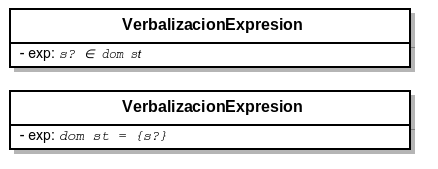
\includegraphics[scale=0.4]{img/mensajes.png}
	\caption{Mensajes a comunicar para el ejemplo de la figura~\ref{fig:ej_test_desc}}
  	\label{fig:ej_mensajes}
\end{figure}

Vale la pena aclarar que en este trabajo, los datos con los que se trabaja resultan esquemas Z de las clases de prueba, por lo que ya se encuentran modelados de antemano y no es necesario realizar un nuevo modelo del dominio.
 

\section{Determinación del contenido}
\label{cap:determinacion_contenido}

Como se mencionó anteriormente, en la \emph{determinación de contenido} se suelen llevar a cabo una o más tareas de \emph{selección}, \emph{resumen} y \emph{razonamiento con los datos}. En la figura \ref{fig:tareas_determinacion_contenido} podemos observar el orden en que se realizarán estas tareas y a continuación estudiaremos cada una de ellas detalladamente.

\begin{figure}[H]
  	\centering
	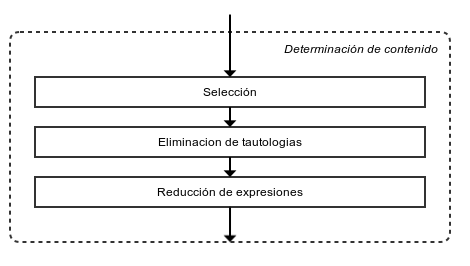
\includegraphics[scale=0.4]{img/tareas_determinacion_contenido.png}
	\caption{Tareas determinación de contenido}
  	\label{fig:tareas_determinacion_contenido}
\end{figure}

\subsection*{Selección}
Como vimos en la sección anterior, nuestro sistema de NLG deberá ser capaz de producir descripciones para un subconjunto de clases de prueba del total de las clases generadas por \emph{Fastest} para una especificación. Es decir, el usuario podría solicitarle a nuestro sistema la generación de descripciones para una, un grupo o todas las clases de pruebas generadas y éste debería generar descripciones únicamente para las clases de prueba indicadas. Es por esto que se debe realizar una \emph{selección de la información} que tendrá que ser incluida dentro del \textit{document plan} a fin de ser comunicada, posteriormente, en el texto final.

Para el caso de nuestro trabajo esta tarea se resumirá a la búsqueda y filtrado de las clases de prueba indicadas por el usuario dentro de todo el conjunto de clases de prueba que forma parte de la entrada del sistema. De forma tal que si, por ejemplo, se desea generar una descripción para la clase de prueba \emph{LookUp\_SP\_1} (del ejemplo introducido en la sección \ref{sec:ej-symbolTable}), la misión de esta tarea será la de identificar y seleccionar la clase \emph{LookUp\_SP\_1} entre todas las generadas por \emph{Fastest} que formarán parte de los datos de entrada de nuestro sistema de NLG.
%TODO falta ref despues de \emph{LookUp\_SP\_1}

%TODO agregar grafico aca para ejemplificar?

Ya seleccionadas las clases de prueba con las que se debe trabajar, veremos cómo podemos mejorar las descripciones de nuestro sistema realizando algunos procesamientos sobre la información seleccionada previo a la construcción del \textit{document plan}. En particular veremos dos tareas que se podrían enmarcar dentro del razonamiento con los datos, la \emph{eliminación de tautologías} y la \emph{reducción de expresiones}. Ambas tareas se realizarán sobre la estructura de los predicados Z, implementando reglas de reescritura para cada uno de los casos. El capítulo \ref{cap:implementacion} se presentará cómo éstas se encuentran implementadas y cómo podremos hacer para agregar nuevas reglas de reescritura a nuestro sistema de NLG\footnote{Las dos tareas de razonamiento trabajan sobre los casos más comúnmente observados dentro del corpus recolectado. Sin embargo, como veremos en el capítulo \ref{cap:conclusion}, será posible mejorar la calidad de las descripciones producidas profundizando sobre la tarea de reducción de expresiones y agregando nuevas nuevas tareas de razonamiento a nuestro sistema.}.

\subsection*{Eliminación de tautologías}
Como se mencionó anteriormente, todas las clases de prueba incluidas en el corpus fueron generadas utilizando \emph{Fastest 1.6}. Se ha observado que en ciertos casos, esta herramienta genera clases de prueba como la que podemos ver a continuación:

\begin{figure}[H]
  \centering
\begin{schema}{Update\_ SP\_ 2}\\
 st : SYM \pfun VAL \\
 s? : SYM \\
 v? : VAL 
\where
 st = \{ \} \\
 \{ s? \mapsto v? \} \neq \{ \}
\end{schema}
  \caption{Clase de prueba para operación Update\_SP\_2}
  \label{fig:ej_update_sp_2}
\end{figure}

Podemos observar en este caso, que la siguiente expresión del ejemplo anterior:

\begin{figure}[H]
  \centering
  $\{ s? \mapsto v? \} \neq \{ \}$ 
\end{figure}

\noindent
no aporta información relevante para el usuario, de hecho esta expresión no agrega ninguna restricción para el caso de prueba ya que será siempre verdadera y si intentáramos describir este predicado, terminaríamos con un texto parecido al siguiente:

\begin{figure}[H]
  \centering
  \emph{``el conjunto formado por el par formado por el símbolo a actualizar y el nuevo valor, es distinto al conjunto vacío''}
\end{figure}

\noindent
que además de resultar algo difícil de interpretar, no contribuye al objetivo comunicacional.

Esto sugiere que se obtendrán descripciones más claras si se filtran este tipo de expresiones. En particular, se debería hacer lo antes posible en el \textit{pipeline} de nuestro sistema y la tarea de determinación de contenido resulta la apropiada para realizar este tipo de procesamiento. De esta forma se evitará que etapas posteriores, como la de \emph{microplanning} o \emph{surface realization} deban ocuparse de la generación de frases que no aportarían más que confusión al texto final.

En la versión de \emph{Fastest} utilizada en este trabajo solo se ha observado la aparición de tautologías similares a la del ejemplo anterior con predicados con la siguiente estructura:

\begin{figure}[H]
  \centering
  $\{ a, b, ... , n \} \neq \{ \}$ 
\end{figure}

\noindent
por lo tanto, la implementación de nuestro sistema solo necesitará considerar el caso antes mencionado. 

En la figura \ref{fig:ej_elim_tauto} podemos ver ilustrado el comportamiento esperado de la tarea de \emph{eliminación de tautologías} para el ejemplo utilizado anteriormente.

\begin{figure}[H]
  	\centering
	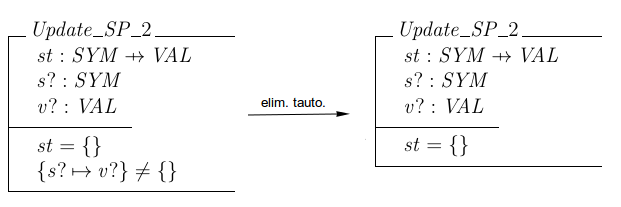
\includegraphics[scale=0.4]{img/ej_elim_tauto.png}
	\caption{Eliminación de tautología para Update\_SP\_2}
  	\label{fig:ej_elim_tauto}
\end{figure}

Será tarea de nuestro \textit{document planner}, entonces, filtrar tautologías presentes en las clases de prueba para asegurarnos de este modo que no sean incluidas dentro del \emph{document plan}.

\subsection*{Reducción de expresiones}
Podemos observar en el corpus que hay algunas expresiones que se podrían simplificar y de esta forma lograr descripciones más claras y concisas. Veamos por ejemplo la figura \ref{fig:ej_update_sp_4}.

\begin{figure}[H]
  \centering
  \begin{schema}{Update\_ SP\_ 4}\\
   st : SYM \pfun VAL \\
   s? : SYM \\
   v? : VAL 
  \where
   st \neq \{ \} \\
   \dom st = \dom \{ s? \mapsto v? \}
  \end{schema}
  \caption[]{Clase de prueba para operación Update\footnotemark}
  \label{fig:ej_update_sp_4}
\end{figure}
\footnotetext{Ésta difiere levemente de la presentada en el Apéndice \ref{ape:corpus}. A fin de simplificar el ejemplo fueron eliminadas las tautologías de la misma.}

En particular observemos la expresión:

\begin{figure}[H]
  \centering
  $\dom st = \dom \{ s? \mapsto v? \}$ 
\end{figure}

Si nos adelantamos un poco y tratamos de verbalizar esta expresión de acuerdo a las reglas presentadas en el capítulo \ref{sec:corpus_reglas} se podría generar una frase como la siguiente:

\begin{figure}[H]
  \centering
  \emph{``el conjunto de símbolos cargados en la tabla es igual al dominio del par formado por el símbolo a actualiza y el nuevo valor''}
\end{figure}

\noindent
que no parece ser la verbalización más adecuada para la expresión dada. Por otro lado, veamos que es posible reducir la expresión anterior a la siguiente expresión equivalente:

\begin{figure}[H]
  \centering
  $\dom st = \{s?\}$ 
\end{figure}

\noindent
esta última expresión resultará más fácil de verbalizar, al menos según las reglas introducidas, nuestro sistema podría generar una descripción similar a la siguiente:

\begin{figure}[H]
  \emph{``el símbolo a actualizar es el único elemento en la tabla de símbolos cargados''}
\end{figure}

El caso presentado anteriormente fue un caso muy recurrente que se notó en las clases generadas por \emph{Fastest}. Éste resulta de la aplicación de la táctica de partición estándar sobre el operador $\oplus$, lo cual es bastante habitual. Es por esto que es importante trabajar este tipo de expresiones antes de incluirlas dentro del \emph{document plan}. Para esto, nuestro \emph{document planner} deberá realizar el siguiente remplazo siempre que sea posible:

\begin{figure}[H]
  \centering
  $\dom \{ x \mapsto y \} \rightarrow \{x\}$ 
\end{figure}

En la figura \ref{fig:ej_reduce} podemos ver ilustrado el comportamiento esperado de la tarea de \emph{reducción de expresiones} para el ejemplo utilizado anteriormente.

\begin{figure}[H]
  	\centering
	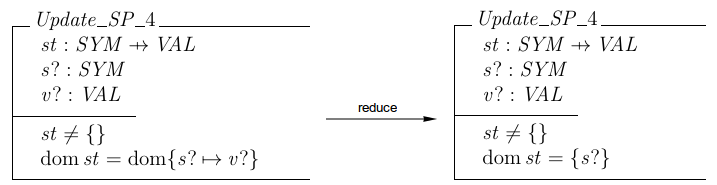
\includegraphics[scale=0.4]{img/ej_reduce.png}
	\caption{Reducción de expresiones para Update\_SP\_4}
  	\label{fig:ej_reduce}
\end{figure}


Será tarea de nuestro \textit{document planner}, entonces, trabajar también este tipo de expresiones antes de construir los mensajes a incluir dentro del \emph{document plan}. 

El caso anterior resulta el más comúnmente observado dentro de las clases de prueba generadas por Fastest y fue el único contemplado dentro del alcance de este trabajo. Sin embargo, veremos en el capítulo \ref{cap:implementacion}, cómo fácilmente podremos introducir a nuestra implementación nuevas reglas, similares a la presentada anteriormente.

\section{Estructuración del documento}
\label{sec:document_structure}

Como se mencionó anteriormente, el texto generado no podrá ser una colección de frases y palabras al azar. Deberá tener coherencia y poseer una estructura que le permita al lector interpretar con facilidad el contenido del mismo. Para esto, necesitaremos considerar cómo organizaremos y estructuraremos la información que se debe comunicar a fin de producir un texto razonablemente fácil de leer y comprender.

%~\footnote{Las decisiones sobre cómo debe estar ordenado y agrupado el documento final son resultado del análisis del corpus de descripciones.}
Esta tarea se concentrará en construir una estructura que contenga la información seleccionada y procesada en la etapa de \emph{determinación de contenido}, estableciendo el agrupamiento y ordenamiento de la misma. Esta estructura deberá caracterizar la disposición de los elementos pertenecientes a los textos recopilados en el corpus. De éste, podemos observar que los documentos a generar poseen una estructura bastante simple y rígida a la vez: están formados por una secuencia de descripciones para las clases de prueba seleccionadas en la etapa de \emph{determinación de contenido}. A su vez, cada una de estas descripciones agrupa los \emph{mensajes} que modelan la verbalización de las expresiones pertenecientes a cada clase, ordenados de la misma forma en la que aparecen en el esquema de la clase de prueba en cuestión. 

Para modelar nuestro \emph{document plan}, utilizaremos un elemento al que llamaremos \emph{DocumentoDP}, este elemento modelará el documento completo (será la raíz de nuestro \emph{document plan}), este elemento contendrá el título para el documento a generar y un conjunto de elementos que modelarán las descripciones de las distintas clases de prueba. Llamaremos \emph{DescripcionClasePrueba} a estos últimos, utilizados para modelar las descripciones de las distintas clases de prueba. Estos estarán formados por información general de la clase de prueba a describir (como el nombre de la misma y una pequeña descripción de la operación a testear\footnote{Esta descripción o encabezado en las \emph{DescripcionClasePrueba} se construirá en base al texto utilizado para designar la operación para la cual fue derivada la clase de prueba en cuestión.}) y un conjunto de los \emph{mensajes} introducidos anteriormente, \emph{VerbalizacionExpresion}, que modelaran las verbalizaciones de las expresiones Z contenidas dentro de las clases de prueba. En la figura~\ref{fig:png_document_plan} podemos observar una representación abstracta de la estructura que tendrá nuestro \emph{document plan}.

\begin{figure}[H]
  	\centering
	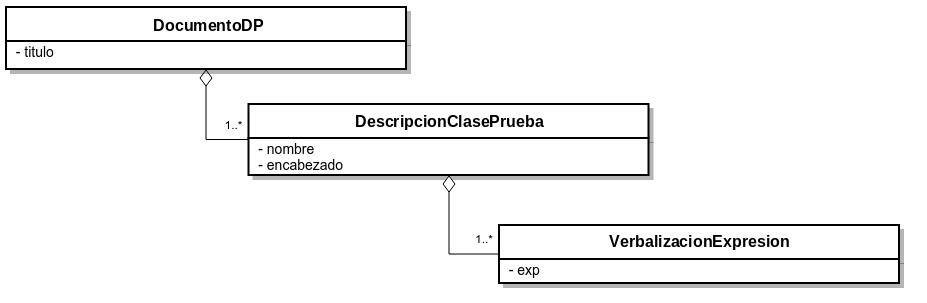
\includegraphics[scale=0.4]{img/document_plan.png}
	\caption{\textit{Document plan}}
  	\label{fig:png_document_plan}
\end{figure}

Podemos ver en la figura~\ref{fig:png_document_plan_ej} un ejemplo del document plan para la descripción de la clase de prueba \emph{LookUp\_SP\_1} utilizada en el capítulo anterior (página \pageref{fig:ej_test_desc}). 

\begin{figure}[H]
  	\centering
	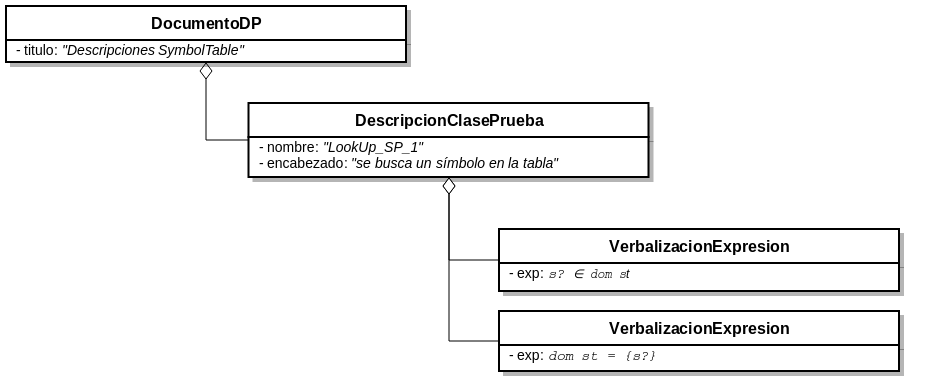
\includegraphics[scale=0.4]{img/document_plan_ej.png}
	\caption{\textit{Document plan} correspondiente al texto de la figura~\ref{fig:ej_test_desc}}
  	\label{fig:png_document_plan_ej}
\end{figure}

\section{Resumen del capítulo}
En este capítulo se analizaron las tareas que debe realizar nuestro \emph{document planner}. Como vimos, la misión del mismo es construir un \emph{document plan} que contenga la información requerida por el usuario, filtrada, procesada y organizada. Se tomaron decisiones generales sobre la estructura del documento, dejando para etapas posteriores el trabajo más detallado, por ejemplo, a nivel de las oraciones. Será tarea del \emph{microplanner}, como veremos el próximo capítulo, procesar los \emph{mensajes} construidos en esta etapa y generar a partir de estos una especificación de frase para cada expresión de Z que debemos verbalizar, así como también transformar los elementos que contienen información estructural en especificaciones más concretas del texto a generar (utilizando elementos que modelarán párrafos, secciones, lista de ítems, etc.).

\chapter{\textit{Microplanning}}
\label{cap:microplanning}

La etapa de \textit{microplanning} será la encargada de, a partir del \textit{document plan} producido por la etapa anterior, producir una especificación más detallada del el texto a generar. 

En éste capítulo presentaremos las tres tareas que, según Reiter y Dale~\cite{reiter_dale}, deberían llevarse a cabo en esta etapa: lexicalización, agregación y generación de expresiones de referencia. Luego definiremos en detalle la entrada y salida del \textit{microplanner}. Finalmente profundizaremos particularmente sobre la tarea de lexicalización que debemos llevar a cabo para este trabajo.

A lo largo de este capítulo continuaremos con el ejemplo utilizado en la etapa anterior, ilustrando cómo a partir del \textit{document plan} presentado en la la figura \ref{fig:png_document_plan_ej} construiremos una especificación más detallada del documento a generar.

\section{Tareas del \textit{Microplanner}}

Como mencionamos previamente, el \textit{microplanner} será el encargado de transformar el \textit{document plan} generado en la etapa anterior en una especificación más refinada del texto a generar. Cabe aclarar que el resultado de esta etapa no será todavía el texto final ya que quedarán por tomar decisiones acerca de la sintaxis, morfología y cuestiones de presentación, de las cuales se encargará el realizador de superficie.

Como mencionamos en el capítulo~\ref{cap:nlg_intro}, dentro de las tareas generalmente realizadas por el \emph{microplanner} podemos destacar las siguientes:

\medskip
\noindent
\textbf{Lexicalización:} esta tarea se encarga de elegir qué palabras particulares y qué constructores sintácticos usar para comunicar la información contenida en el \textit{document plan}. Desarrollaremos más en detalle el trabajo realizado por esta etapa en la sección~\ref{sec:microplanning_lexicalization}


\medskip
\noindent
\textbf{Agregación:} la función de esta tarea es la de combinar los elementos informativos del \emph{document plan} con el fin de conseguir un texto más fluido y legible. La agregación decide qué elementos se pueden agrupar para generar oraciones generalmente más complejas sin modificar el significado de las mismas. Por ejemplo, consideremos las siguientes dos descripciones posibles para la clase de prueba \emph{LookUp\_SP\_1} (figura \ref{fig:ej_corpus}):


\begin{center}
\begin{enumerate}
  \item \emph{El símbolo a buscar pertenece a los símbolos cargados en la tabla. El símbolo a buscar es el único elemento de los símbolos cargados en la tabla.} 
  \item \emph{El símbolo a buscar pertenece a los símbolos cargados en la tabla y éste es el único elemento de los símbolos cargados en la tabla.}
\end{enumerate}
\end{center}

\medskip
\noindent
Para este trabajo, decidimos expresar nuestras descripciones siguiendo el estilo de la primer frase del ejemplo anterior, por lo cual nuestro \textit{microplanner} no realizará tareas de agregación. En nuestro caso en particular creemos que será útil para el lector que cada oración de una descripción haga referencia a una única restricción del esquema de la clase de prueba. De esta forma podríamos identificar con mayor facilidad cuál es la descripción para cada expresión particular de una clase de prueba.


\medskip
\noindent
\textbf{Generación de expresiones de referencia:} esta tarea se encarga de determinar qué frases deben ser usadas para identificar las diferentes menciones al mismo elemento en un texto a fin de aportar fluidez a éste. Más específicamente, en los casos que se hace referencia a una entidad que ya ha aparecido en el texto se puede remplazar la misma por otra frase que la referencie. La elección de qué expresión utilizar para referirse a la entidad dependerá del contexto y deberá hacerse sin introducir ambigüedad para el lector. Por ejemplo, en la segunda alternativa presentada anteriormente para describir la clase de prueba \emph{LookUp\_SP\_1}:

\begin{center}
 \emph{\textbf{El símbolo a buscar} pertenece a los símbolos cargados en la tabla y \textbf{éste} es el único elemento de los símbolos cargados en la tabla.}
\end{center}

\noindent
Reemplazamos la segunda ocurrencia de ``el símbolo a buscar'' por el pronombre ``éste''.

\smallskip
Al igual que la tarea de agregación, la generación de expresiones de referencia excede el alcance de este trabajo y  nuestro \textit{microplanner} no realizará tareas este tipo. Sin embargo, en el capítulo \ref{cap:conclusion} propondremos, como un posible trabajo a futuro, la inclusión de las tareas agregación y generación de expresiones de referencia a nuestro sistema. 

%TODO en trabajo futuro se puede relacionar la agregacion con generacion de expresiones de referencia. Diciendo que la inclusion de tareas de agregacion probablemente requieran tareas de generacion de expresiones de referencia para la generacion de textos más fluidos.


\section{Entrada y salida del \textit{microplanner}}
La entrada del \textit{microplanner} será un \textit{document plan} producido por la etapa anterior. Observemos por ejemplo el \textit{document plan} presentado en la figura \ref{fig:png_document_plan_ej} del capítulo anterior, utilizado para modelar la descripción de la clase de prueba \emph{LookUp\_SP\_1}. Esta abstracción no especifica las frases que nuestro sistema debe generar, ni si deben estar enumeradas en una lista de ítems o agrupadas en secciones, por ejemplo. Necesitaremos una especificación más concreta, un modelo más detallado del documento y de las frases a generar. Será entonces responsabilidad del \textit{microplanner}  construir a partir del \textit{document plan} una especificación más concreta del texto a generar.

Llamaremos especificación del texto a la especificación resultado de esta etapa. Ésta se encargará de modelar los distintos elementos que compondrán el texto final (como párrafos, lista de ítems, etc.). Esta especificación estará compuesta en base a especificaciones de frase encargadas de modelar las distintas oraciones que serán incluidas en el texto final (veremos que cada una de estas se construirán a partir de los mensajes contenidos en el \textit{document plan}). Será luego tarea de la siguiente etapa convertir los nodos internos de la especificación del texto en anotaciones especificas para el sistema de presentación\footnote{Llamamos sistemas de presentación a los sistemas encargados de post-procesar las anotaciones antes mencionadas y presentarle al usuario el documento de manera apropiada. Por ejemplo, \LaTeX, Microsoft Word o web browsers como Firefox o Chrome son algunos de los posibles sistemas de presentación.} (realización de estructura) y transformar las especificaciones de frase en oraciones o frases sintáctica, morfológica y ortográficamente correctas (realización lingüística). 

%para que luego, en la etapa de realización de superficie podamos generar el texto final en base a los requerimientos analizados en el capítulo \ref{cap:corpus}. 

En lo que queda de esta sección estudiaremos cómo se encuentra constituida nuestra especificación del texto, describiendo también cómo están formadas nuestras especificaciones de frase.

\subsection{Especificación del texto}

%TODO faltaría explayar un poco más y hablar sobre conceptos de phrase y text specification
%Como vimos en el capítulo anterior, la salida del  \textit{document planner} es una estructura donde se encuentran agrupados los elementos informativos que deseamos comunicar. Estos elementos o \emph{mensajes} contenidos en el \emph{document plan} especifican de una manera abstracta la información que debemos comunicar en el texto final, pero no especifican, por ejemplo, que palabras debemos usar para hacerlo. 

%Será el \textit{microplanner} el encargado de tomar este tipo de decisiones. Éste tomará como entrada un \textit{document plan} y deberá producir una especificación más refinada del texto que deseamos generar, la cual será utilizada luego por el \emph{realizador de superficie} para producir el texto final.

La especificación de texto para nuestro sistema, deberá caracterizar la estructura del documento final que nuestro sistema debe producir. Es por esto que modelaremos los mismos utilizando un árbol, donde los hojas especificarán las frases u oraciones a generar (las especificaciones de frase), y los nodos internos establecerán cómo estas frases tendrán que ser agrupadas en elementos del documento (como párrafos, secciones, lista de ítems, etc). 

La estructura de los documentos que debemos generar en este trabajo resulta relativamente simple. Como vimos en el capítulo \ref{cap:corpus}, los documentos de descripciones poseen un título y luego se detallan una por una las descripciones de las distintas clases de prueba, donde para cada una de éstas aparece el nombre de la clase de prueba, junto a una pequeña descripción de la operación a testear y luego una lista de ítems que describirán cada una de las restricciones pertenecientes a la clase de prueba que se describe. Es por esto que para este trabajo utilizaremos sólo dos elementos para modelar la estructura interna del documento \emph{TSDocumento} y \emph{TSListaItems}:

\medskip
\noindent
\textbf{TSDocumento:} modela el documento final, por lo tanto solo tendremos un elemento de este tipo en nuestra especificación del texto y éste será la raíz del documento. Éste elemento contendrá información general sobre el documento, como el título y una especificación para cada descripción de clase de prueba, modeladas mediante \emph{TSListaItems}.

\medskip
\noindent
\textbf{TSListaItems:} modela el texto que describirá a una clase de prueba. Este elemento contiene una especificación de frase que modelará el texto correspondiente al título y al detalle de la descripción. Además contendrá una lista de especificaciones de frase que especificarán las frases para cada una de las verbalizaciones de las expresiones contenidas en la clase de prueba en cuestión. Habrá una \emph{TSListaItems} por cada clase de prueba a describir.

\begin{figure}[H]
  	\centering
	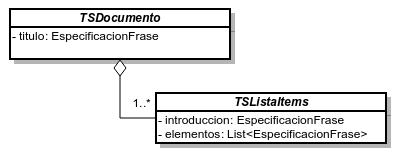
\includegraphics[scale=0.3]{img/text_spec.png}
	\caption{Especificación de texto.}
  	\label{fig:text_spec}
\end{figure}

En la figura anterior podemos observar la estructura abstracta que tendrán nuestras especificaciones del texto y por ejemplo, sin meternos en detalle todavía sobre la estructura de las especificaciones de frase, en la figura \ref{fig:text_spec_ej} podemos ver una especificación de frase para el ejemplo introducido anteriormente (página \pageref{fig:ej_corpus}).

\begin{figure}[H]
  	\centering
	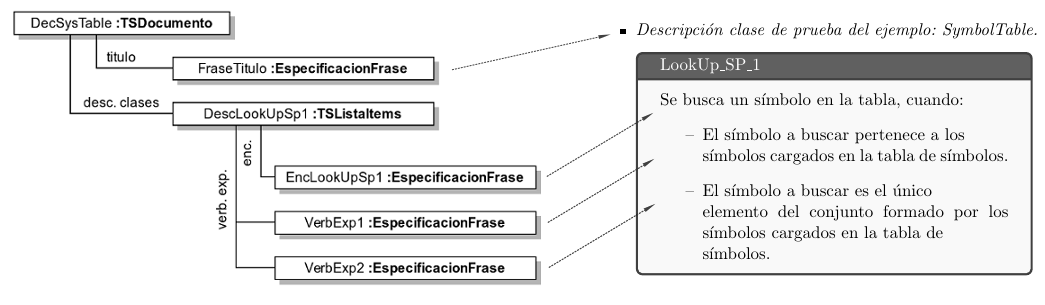
\includegraphics[scale=0.35]{img/ej_text_spec.png}
	\caption{Ejemplo especificación del texto.}
  \label{fig:text_spec_ej}
\end{figure}

Veremos en el próximo capítulo cómo, en la etapa de realización estructural, transformaremos estos elementos en anotaciones para el sistema de presentación.

\subsection{Especificación de frase}

En la literatura sobre NLG podemos encontrar muchas alternativas en lo que respecta a la especificación de frases (\textit{skeletal propositions}, \textit{meaning specifications} y \textit{lexicalised case frames} entre otras \cite{reiter_dale}). Todas éstas varían en el nivel de abstracción que poseen. Las representaciones más abstractas le darán más flexibilidad a las etapas de \textit{document planning} y \textit{microplanning}, pero al mismo tiempo nos obligarán a tener un realizador de superficie más sofisticado. Por otro lado, las especificaciones menos abstractas, requieren que el \textit{document planner} y el \textit{microplanner} realicen un mayor trabajo, pero también tendrán más control sobre el texto a producir. Uno de los objetivos que tuvimos a la hora de idear una estructura para nuestra especificación de frases fue que ésta sea independiente de nuestro problema; pretendemos que hable en términos de la lengua (castellano en nuestro caso) que queremos generar y no en términos específicos de Z. Es por esto que decidimos especificar las oraciones a generar mediante árboles sintácticos, donde los constituyentes de éstos son los sintagmas de la oración que deseamos generar. Esto le dará la posibilidad al realizador lingüístico de poder identificar la función de cada uno de los constituyentes de la oración. Por ejemplo, como detallamos en los requerimientos de la sección \ref{sec:corpus_gramatica}, el \emph{realizador de superficie} necesitará identificar el núcleo de un sintagma nominal (núcleo del sujeto) para poder producir una oración en la que haya concordancia de número y persona entre el verbo y el sujeto. Como consecuencia del ejemplo anterior, nuestro realizador lingüístico deberá proveerle al realizador de superficie una especificación que permita identificar el sujeto, predicado y verbo de una oración. Creemos que con los elementos presentes en la figura~\ref{fig:phase_spec} podremos modelar la frases incluidas en el corpus.

\begin{figure}[h]
  	\centering
	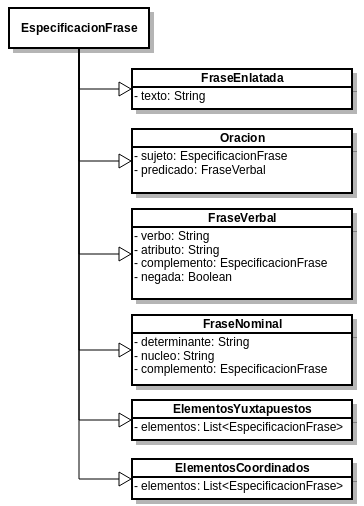
\includegraphics[scale=0.7]{img/phrase_spec.png}
	\caption{Especificación de frase.}
  	\label{fig:phase_spec}
\end{figure}

No pretendemos modelar toda la lengua castellana con estos elementos sino solo un subconjunto que nos provea las herramientas necesarias para permitirle al \emph{realizador de superficie} generar las frases definidas en el capítulo \ref{sec:corpus_analisis}, ya que el desarrollo de un realizador lingüístico que considere todas las construcciones sintácticas de nuestra lengua escapa el alcance de este trabajo. Es por esto que sólo modelamos los sintagmas nominales (FraseNominal) y verbales (FraseVerbal) y nos vemos obligados a incluir otros elementos como ElementosYuxtapuestos para salvaguardar la falta de algunos constituyentes sintácticos como sintagmas adjetivales, preposicionales, etc. 

A continuación describiremos brevemente cada uno de estos elementos, profundizando sobre la realización de los mismos en el capítulo \ref{cap:linguistic_realization}.


\medskip
\begin{itemize}
\item{\emph{\textbf{FraseEnlatada}}: Representa texto que no necesita ningún tipo de procesamiento posterior a realizar durante la realización lingüística, será incluido en el texto tal cual fue establecido.}
\item{\emph{\textbf{Oracion}}: Modela oraciones bimembres. El realizador lingüístico deberá procesarlas en base a una serie de reglas gramaticales para producir un texto sintáctica, morfológica y ortográficamente correcto para éstas.}
\item{\emph{\textbf{FraseVerbal}}: Representa un sintagma verbal que corresponderá al predicado de una \emph{Oración}.}
\item{\emph{\textbf{FraseNominal}}: Modela un sintagma nominal. Generalmente conformará el sujeto en una \emph{Oración}.}
\item{\emph{\textbf{ElementosCoordinados}}: Representa una serie de elementos que se deberán transformar en una conjunción de frases en la etapa de realización lingüística, por ejemplo: \emph{``frase1\textbf{,} frase2 \textbf{y} frase3''}}
\item{\emph{\textbf{ElementosYuxtapuestos}}: Representa una lista ordenada de elementos que deberán ser realizados y \emph{concatenados} en la oración final. Nos vimos obligados a introducir este tipo de elementos para salvaguardar la falta de algunos constituyentes sintácticos como sintagmas adjetivales, preposicionales, etc.}
\end{itemize}

\bigskip
En la siguiente sección veremos cómo la tarea de lexicalización construirá estas especificaciones de frase en base a la información contenida en los mensajes del \textit{document plan}.
%\section{Arquitectura}

\section{Lexicalización}
\label{sec:microplanning_lexicalization}

Como mencionamos anteriormente, el proceso de lexicalización será el encargado de elegir qué palabras particulares y constructores sintácticos usar para comunicar la información contenida en el \textit{document plan}. En esta etapa deberemos producir una especificación de frase para cada mensaje contenido en el \textit{document plan}. En nuestro caso debemos hacerlo contemplando todos los casos definidos en el capítulo \ref{sec:corpus_reglas}, es decir, nuestro proceso de lexicalización tendrá que comportarse de forma similar a la función \texttt{verb} que estudiamos durante el análisis de requerimientos. Tanto las palabras, como los sintagmas a utilizar se desprenderán de las frases presentes en la definición de \texttt{verb}.

Como analizamos en el capítulo \ref{cap:corpus}, nuestro sistema deberá producir una oración en lenguaje natural para cada predicado incluido dentro del cuerpo de cada clase de prueba, a su vez, la verbalización para cada una de estas expresiones se encuentra caracterizada por un mensaje dentro del \textit{document plan}. Es por esto que el módulo encargado de esta tarea deberá ser capaz de generar una \emph{especificación de frase} a partir de la expresión Z contenida en cada uno de estos mensajes. De acuerdo a los requerimientos introducidos en el capítulo \ref{cap:corpus}, nuestro lexicalizador primero deberá verificar si la expresión en cuestión se encuentra designada, en este caso, tendrá que construir una especificación de frase en base a su designación. De lo contrario deberá intentar construirla recursivamente contemplando los casos para los distintos operadores y las posibles combinaciones. En el algoritmo~\ref{fig:algoritmo_lexicalizacion} podemos ver un bosquejo del comportamiento esperado para esta tarea, de acuerdo al análisis realizado en la sección \ref{sec:corpus_reglas}, trabajando esta vez con las especificaciones de frase definidas en la sección anterior. Incluimos sólo un bosquejo ya que ilustrar el comportamiento completo de esta tarea resulta extenso debido a la construcción y composición de elementos que debemos realizar para cada caso; en particular incluimos un caso para la lexicalización del operador $\in$ que utilizaremos posteriormente para desarrollar el ejemplo que presentaremos en la figura \ref{fig:phase_spec_ej}.

%TODO ver como cambiar el caption de esto
\begin{algorithm}[H]
\caption{Bosquejo de \textsc{lexicalizacion} para el operador $\protect\in$.}\label{fig:algoritmo_lexicalizacion}
\begin{algorithmic}[1]
\Function {lexicalizacion}{exp}
\If{\Call{esta\_designada}{exp}}
\State ret $\gets$ \Call{designacion}{exp}
\Else
\State ret $\gets$ \Call{lexicalizacion'}{exp}
\EndIf
\State \textbf{return} ret
\EndFunction
\Statex
\Function {lexicalizacion'}{x $\protect\in$ y}
\State oracion.sujeto $\gets$ \Call{lexicalizacion}{x}
\State fraseVerbal.verbo $\gets$ \text{\textit{``pertenece''}}
\State fraseEnlatada.texto $\gets$ \text{\textit{``a''}}
\State elemYuxtapuesto.elementos $\gets$ \{fraseEnlatada, \Call{lexicalizacion}{y}\}
\State fraseVerbal.complemento $\gets$ elemYuxtapuesto
\State oracion.predicado $\gets$ fraseVerbal
\State \textbf{return} oracion
\EndFunction
\end{algorithmic}
\end{algorithm}

La función \textsc{designacion} deberá ser capaz de construir una especificación de frase a partir de una expresión designada. Analizaremos este caso con mayor profundidad en la siguiente sección. Por otro lado, notemos que en el caso que la expresión a lexicalizar no se encuentre designada, se deberá analizar recursivamente la expresión para generar el texto adecuado. 

A continuación, retomaremos el ejemplo de la figura \ref{fig:text_spec} y veremos cómo deberá nuestro sistema generar la especificación de frase para uno de los mensajes incluido en el \textit{document plan}. En la figura \ref{fig:phase_spec_ej} podemos observar este mensaje y el resultado de la lexicalización del mismo. Veremos a continuación los pasos que deberá realizar nuestro sistema durante la tarea de lexicalización para lograr el resultado ilustrado en la imagen.

%A continuación detallaremos los pasos realizados por nuestra tarea de lexicalización para obtener dicho resultado.

\begin{figure}
  	\centering
	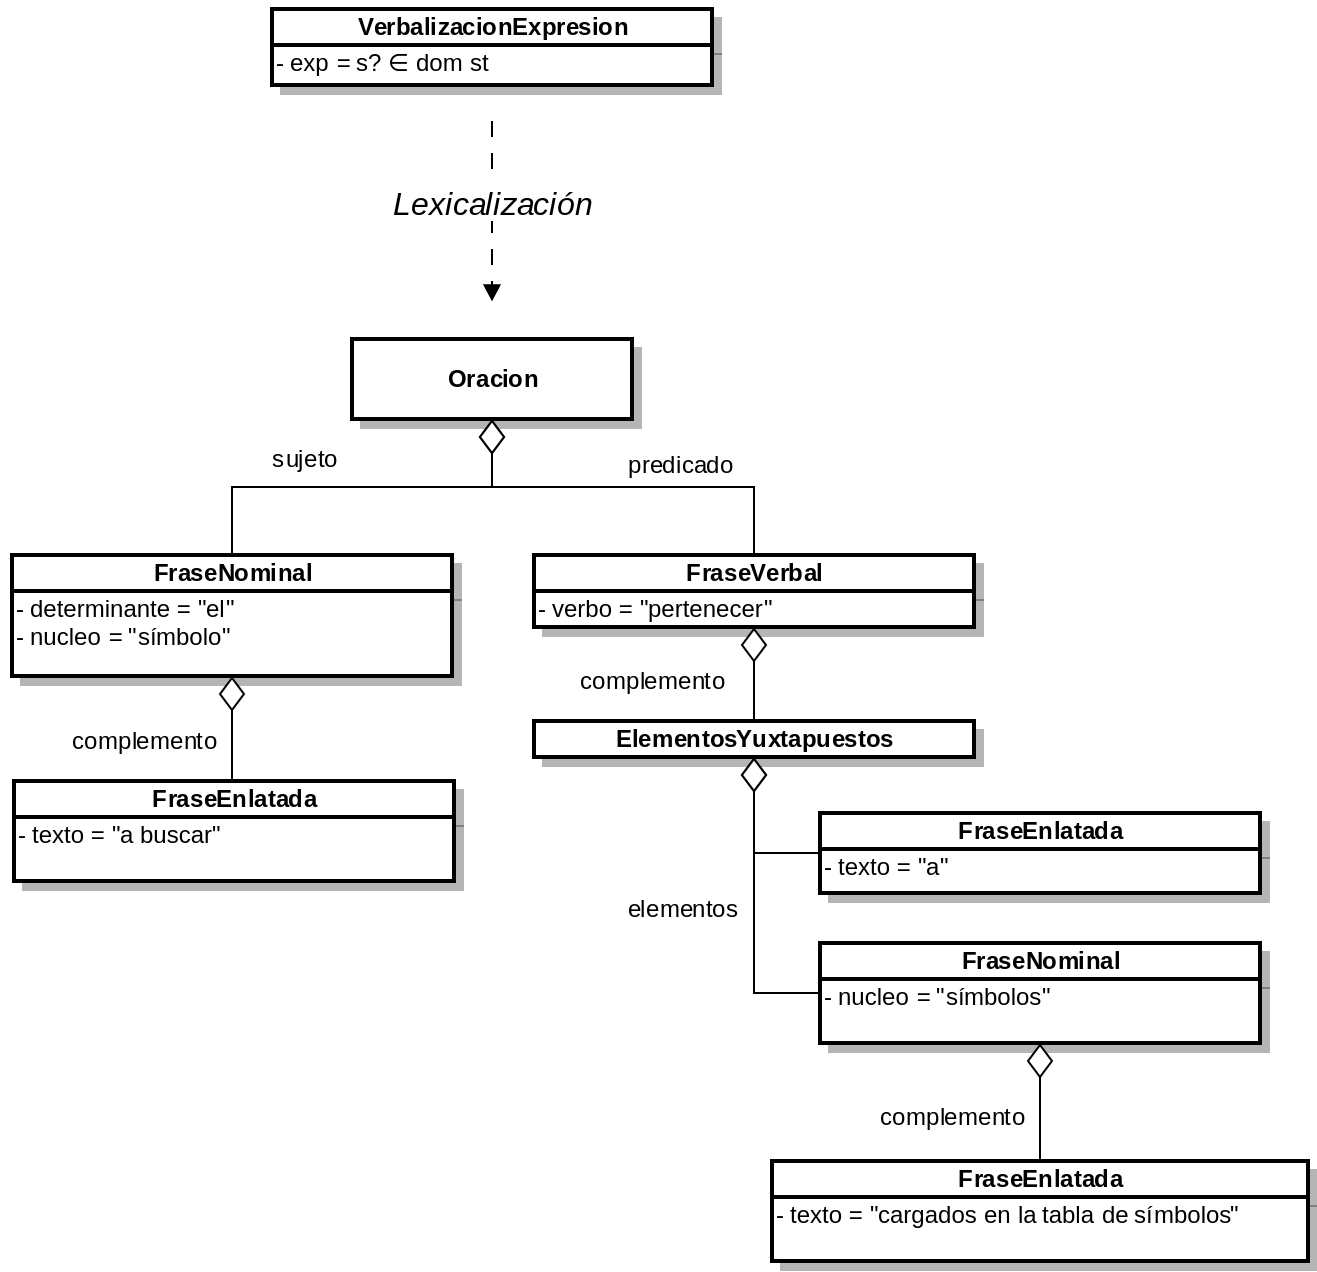
\includegraphics[scale=0.25]{img/phrase_spec_ej.png}
	\caption{Especificación de frase para $s? \protect\in \protect\dom st$.}
  	\label{fig:phase_spec_ej}
\end{figure}

El objetivo del lexicalizador será construir una especificación de frase escogiendo adecuadamente las palabras y constructores sintácticos para siguiente la expresión:

\begin{center}
$s? \in \dom st$
\end{center}

\noindent
Asumimos que contaremos con las siguientes designaciones:

%TODO ver esto
\begin{figure}[H]
\begin{align*} 
  &s? && \approx \text{el símbolo a buscar} \\
  &dom~st && \approx \text{símbolos cargados en la tabla de símbolos}
\end{align*}
\end{figure}

En primer instancia, al no encontrarse designada $s? \in \dom st$ nuestro lexicalizador intentará construir la especificación en base a los operadores que componen la expresión a describir. En el algoritmo \ref{fig:algoritmo_lexicalizacion} incluimos el caso para lexicalizar el predicado $x \in y$ que deberemos utilizar para lexicalizar $s? \in \dom st$. 

Será necesario lexicalizar recursivamente las expresiones: $s?$ y $\dom st$. El resultado de estas lexicalizaciones será usado para construir el sujeto y parte del predicado de la oración a especificar. Estas expresiones se encuentran ambas designadas y por lo tanto su especificación de frase se construirá a partir del texto incluido en sus designaciones. Veremos luego en la siguiente sección la tarea de la función \textsc{designacion} utilizada en el algoritmo anterior encargada de producir una especificación de frase a partir de una expresión designada. 

Como ya mencionamos, utilizaremos el resultado de la lexicalización de $s?$ para formar el sujeto de la oración que deseamos especificar y deberemos luego construir la \emph{FraseVerbal} que cumplirá el rol de predicado. Para construir esta última usaremos la especificación de frase que modelará la verbalización $\dom st$, también mencionada anteriormente. 

Finalmente escogeremos las palabras indicadas a fin de que nuestro sistema pueda dar con una descripción similar a la presentada en el capítulo \ref{sec:corpus_reglas} del análisis de requerimientos. Notemos que para esto utilizamos el verbo ``pertenecer'', en infinitivo, siendo luego tarea del realizador lingüístico la de conjugar el mismo de acuerdo a las reglas gramaticales introducidas en la sección~\ref{sec:corpus_gramatica}. Otra cuestión a mencionar es el uso del elemento \emph{ElementoYuxtapuestos} para salvaguardar la falta de un elemento que nos sirva para modelar un sintagma preposicional en este caso. Nuestro realizador lingüístico deberá procesar los elementos contenidos en cada \emph{ElementoYuxtapuestos} generando un texto resultado de la concatenación de la realización los mismos.

A continuación, en la siguiente sección estudiaremos finalmente, la lexicalización de expresiones designadas.

%TODO cambiar nombre
\section{Lexicalización de expresiones designadas}
\label{sec:verbalizacion_designaciones}
Como vimos en la sección anterior, nuestra tarea de lexicalización deberá hacer uso de las designaciones presentes en la especificación para la construir una especificación de frase. Para esto, cuando una expresión se encuentre designada, nuestro sistema tendrá que procesar la designación, construyendo una especificación de frase que la caracterice. Esto será necesario ya que, como mencionamos previamente, en la etapa de \emph{realización de superficie} nuestro sistema necesitará conocer los distintos constituyentes sintácticos de las oraciones que les provee la especificación de frase y en algunos casos también deberá modificar levemente los textos presentes en las designaciones (por ejemplo, como mencionamos en la sección \ref{sec:corpus_gramatica}, puede ser necesario agregarle el artículo correspondiente a la frase utilizada en la designación).

Para este trabajo, estudiaremos por separado las designaciones parametrizadas y las no parametrizadas.

Comencemos por analizar la lexicalización de una expresión que se encuentra designada por medio de una designación no parametrizada. Por ejemplo, supongamos que queremos construir una especificación de frase para la expresión $s?$ del ejemplo utilizado en la sección anterior. Recordemos que la designación para la misma es:

\begin{center} 
  $s? \approx \text{el símbolo a buscar}$ 
\end{center}

La oración utilizada en la designación anterior, como en los casos observados en el corpus (para designaciones no parametrizadas) resulta un \emph{sintagma nominal}. En este caso ``símbolo'' es el núcleo, ``el'' cumple la función de determinante y ``a buscar'' es el complemento. Será posible entonces, para nuestra tarea de lexicalización, modelar estas frases utilizando una \emph{FraseNominal}. 

Para que nuestro sistema sea capaz de esto deberá analizar sintácticamente las designaciones, \textit{parseando} las mismas con la ayuda de un analizador morfológico que nos permitirá obtener la función sintáctica de cada constituyente de la frase. Además de esto, para simplificar la tarea de \emph{parseo} de nuestro sistema, requeriremos que el usuario escriba las designaciones mediante un sintagma nominal. Es decir, respetando la siguiente estructura:

\begin{figure}[H]
  \centering
   \textbf{Sintagma Nominal} = [\textbf{Determinante}] + \textbf{Núcleo} + [\textbf{Complemento}]
\end{figure}

En el capítulo \ref{cap:implementacion} veremos más en detalle cómo utilizamos un analizador morfológico para ayudarnos con la especificación de las frases incluidas en las designaciones.

Por otro lado, las frases incluidas en las designaciones parametrizadas no poseen la misma estructura. La tarea de modelar minuciosamente estos textos resulta más compleja que para el caso anterior. Por ejemplo, podríamos tener uno o más parámetros presentes dentro del texto, para los cuales deberíamos identificar el rol que cumple cada uno de los anteriores dentro de la oración. Además, nuestro realizador lingüístico sólo soportará oraciones de la forma SVO (sujeto, verbo, objeto) lo cual podría no respetarse en una designación introducida por el usuario. Es por esto que nuestro sistema proveerá solo soporte parcial para las designaciones parametrizadas, aceptando sólo designaciones con un único parámetro. Para describir una expresión parametrizada requeriremos a su vez que el argumento de la misma también se encuentre designado. De esta forma podríamos describir una designación parametrizada de la misma forma que vimos en el capítulo \ref{cap:corpus} reemplazando el parámetro presente en el texto de la designación por el texto incluido en la designación del argumento.

Veamos por ejemplo las siguientes designaciones para una especificación que modela un pequeño sistema de monitoreo de sensores\footnote{Cambiamos el dominio debido a que el ejemplo de la tabla de símbolos no presenta un caso adecuado para ilustrar este problema.} incluido en el corpus (apéndice \ref{ape:corpus}):

\begin{figure}[H]
\begin{align*} 
  &x \in \dom smax && \approx \text{x es un identificador válido} \\
  &s? && \approx \text{el identificador del sensor leído}
\end{align*}
\end{figure}

Donde para describir la expresión $s? \in \dom smax$ bastará con reemplazar el parámetro dentro del texto de la designación parametrizada con el texto incluido en la designación de $s?$ como vemos en la figura \ref{fig:ej_lexicalizacion_desig}.

\begin{figure}[H]
  	\centering
	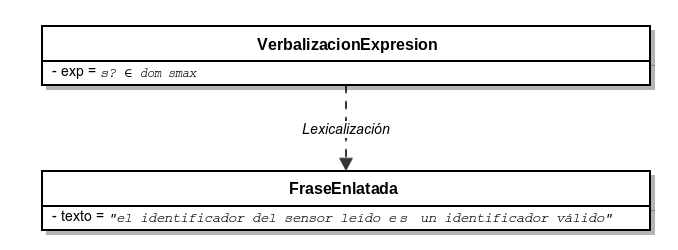
\includegraphics[scale=0.5]{img/ej_lexicalizacion_desig.png}
	\caption{Lexicalización $s? \protect\in \protect\dom smax$.}
  	\label{fig:ej_lexicalizacion_desig}
\end{figure}

Como podemos observar en el ejemplo anterior, al desconocer la estructura del texto presente en las designaciones parametrizadas, deberemos modelar el texto producido por la composición de ambas designaciones utilizando una \emph{FraseEnlatada}. Luego, el texto contenido en estos elementos será realizado sin ningún procesamiento previo, por lo que será responsabilidad del especificador (encargado de escribir las descripciones) que el mismo sea sintáctica y ortográficamente correcto.

\section{Resumen del capítulo}
En este capítulo vimos las tareas necesarias para, partiendo de la salida producida por el \textit{document planner}, constituir una especificación más refinada del texto final. En el próximo capítulo veremos finalmente las tareas que deberán llevarse a cabo para transformar esta especificación del texto en el documento final que contendrá todas las descripciones requeridas por el usuario.


\chapter{Realización de superficie}
\label{cap:realization}
En los capítulos anteriores vimos los procesos que necesitan ser llevados a cabo para lograr una especificación del texto a generar. Finalmente, en esta última etapa nos concentraremos en estudiar las tareas que deben ser realizadas a fin de transformar esta especificación en texto de superficie, formado por frases, símbolos de puntuación y algunas etiquetas de mark-up necesarias.

En las próximas secciones introduciremos las tareas que deberemos llevar a cabo durante esta etapa, repasaremos brevemente la entrada y salida de la misma y finalmente estudiaremos en detalle las tareas de \emph{realización estructural} y \emph{realización lingüística} realizadas en este trabajo.

%Como mencionamos en el capítulo~\ref{cap:microplanning}, nuestra especificación del texto es un árbol en el que las hojas representan las frases individuales y los nodos internos establecen como éstas están agrupadas (según estructuras como párrafos, secciones, listas de ítems, etc). En base a esta diferenciación entre los elementos de nuestra especificación del texto podemos distinguir dos grandes aspectos dentro de esta tarea: la \emph{realización estructural} responsable de transformar los nodos internos de nuestra especificación de texto en anotaciones particulares del sistema de presentación y por otro lado, la tarea de \emph{realización lingüística} que se concentrará en generar frases sintáctica, morfológica, ortográficamente correctas.
%Además, como señalamos en el capítulo~\ref{sec:corpus_analisis}, deberemos agregar un artículo como determinante en el caso de ser necesario. 

\section{Tareas del realizador de superficie}

Como mencionamos en el capítulo \ref{cap:nlg_intro} el realizador de superficie será el encargado de transformar la especificación del texto producida en la etapa de \textit{microplanning} en el documento final. Deberá transformar esta representación abstracta del documento en frases, símbolos de puntuación y algunas etiquetas de mark-up necesarias (estas últimas dependerán del sistema de presentación utilizado).

En el capítulo anterior vimos que la especificación del documento es un árbol, cuyas hojas son especificaciones de frases y sus nodos internos representan cómo las anteriores se deberán estar agrupadas en el documento final (en general estos nodos representan: secciones, párrafos, lista de ítem, etc). Para transformar esta especificación en texto de superficie nuestro realizador deberá llevar a cabo dos tareas: \emph{realización estructural} y \emph{realización lingüística}. La primera se encargará de \emph{mapear} los nodos internos antes mencionados en anotaciones para el sistema de presentación a utilizar. Por otro lado, la realización lingüística deberá convertir las especificaciones de frase en oraciones sintáctica, morfológica y ortográficamente correctas.

En la sección \ref{cap:structure_realization} veremos en detalle la tarea de \emph{realización estructural} que llevaremos a cabo en este trabajo y al final de este capítulo, en la sección \ref{cap:linguistic_realization}, estudiaremos las tareas involucradas en la \emph{realización lingüística} de nuestro sistema de NLG.

\section{Entrada y salida del realizador de superficie}

El objetivo del realizador de superficie será transformar la especificación abstracta del documento, producida por la etapa de \textit{microplanning} en texto de superficie. Este texto estará formado por anotaciones dependientes del sistema de presentación y oraciones generadas por la tarea de realización lingüística.

Será la tarea de realización lingüística la encargada de que en el documento final tengamos una oración por cada especificación de frase incluida en la especificación del texto. Por otro lado, las anotaciones para el sistema de presentación serán generadas por la realización estructural, siendo entonces ésta claramente dependiente del sistema de presentación utilizado. Por ejemplo, si nuestro sistema debe producir un documento latex para luego ser compilado y generar un PDF, será el realizador de superficie (más específicamente de la tarea de realización estructural) el responsable de producir el código necesario para que luego éste se compile apropiadamente. Por ejemplo, en la figura \ref{fig:text_spec} podemos observar un documento producido para la especificación del texto de la figura \ref{fig:ej_latex}.

\begin{figure}[H]
  \begin{verbatim}
  \documentclass{article}
  \title{Descripción clase de prueba del ejemplo: SymbolTable}
  
  \begin{document}
  \maketitle

  LookUp\_SP\_1: Se busca un símbolo en la tabla.  
  Cuando:
  \begin{itemize}
    \item{El símbolo a buscar pertenece ...}
    \item{El símbolo a buscar es el único ...}   
  \end{itemize}
  
  \end{document}
  \end{verbatim}
  \caption{Texto final en \LaTeX.}
  \label{fig:ej_latex}
\end{figure}

A continuación, en las próximas secciones, estudiaremos las tareas de realización estructural y lingüística realizadas para este trabajo.

\section{Realización estructural}
\label{cap:structure_realization}

%La tarea de realización estructural puede resultar relativamente sencilla, pero es importante que se realice por separado a fin de poder generar textos para distintos sitemas de presentacion utilizando la misma realizacion linguistica. Es decir, separar las cuestiones del sistema de presentacion utilizado de las frases u oraciones generadas por nuestro sistema.

Esta tarea deberá transformar los constructores lógicos existentes en la especificación del texto en constructores del sistema de presentación. La mayoría de los sistemas de procesamiento de texto nos permiten indicar mediante el uso de símbolos o etiquetas la naturaleza de una estructura determinada; estas luego estas serán procesadas y renderizadas de manera apropiada permitiéndole al lector una correcta visualización. Por ejemplo, para crear una lista en latex, debemos utilizar el entorno \emph{itemize}, para lo cual tenemos que inicializar y terminar el mismo mediante las sentencias \verb|\begin{itemize}| y \verb|\end{itemize}| respectivamente y entre las anteriores utilizar el comando \verb|\item| para indicar los elemento de la lista.

Es evidente que esta etapa será dependiente del sistema de presentación escogido para el documento final y a su vez independiente del proceso de realización lingüística de la las oraciones o frases a generar.  Por ejemplo, podemos observar en la figura~\ref{fig:ej_latex} de la sección anterior el código latex resultado de la realización de superficie para la especificación de frase introducida en el capítulo anterior (cap. \ref{fig:text_spec}). En la figura~\ref{fig:ej_html} podemos ver otra la realización para la misma especificación de texto pero en lenguaje HTML, donde es posible notar que el texto contenido en ambos ejemplos es exactamente el mismo, diferenciándose únicamente en las anotaciones utilizadas para cada sistema de presentación.

\begin{figure}[H]
  \begin{verbatim}
<html>
<body>
  <h1>Descripción clase de prueba del ejemplo: SymbolTable</h1>

  LookUp_SP_1: Se busca un símbolo en la tabla.  
  <ul>
    <li>Cuando:</li>
    <ul>
      <li>El símbolo a buscar pertenece ...</li>
      <li>El símbolo a buscar es el único ...</li>
    </ul>
  </ul>

</body>
</html>
  \end{verbatim}
  \caption{Texto final en HTML.}
  \label{fig:ej_html}
\end{figure}


A continuación, estudiaremos la tarea de realización estructural para nuestro sistema asumiendo que debemos generar únicamente código latex para luego ser compilado y convertido a un archivo PDF, resultando esto fácilmente extensible para la generación de código para otros sistemas de presentación. Para esto, tenemos que considerar cómo \emph{mapear} los dos constructores lógicos de nuestra especificación de texto anotaciones o sentencias de latex. Para realizar \emph{TSDocumento} deberemos agregar las etiquetas de encabezado necesarias, especificar el tipo del documento, su título título y tendremos que delimitar el principio y final del texto a incluir en el documento. Luego deberemos realizar recursivamente los elementos contenidos en el documento (\emph{TSListaItems}) y ubicarlos adecuadamente en el cuerpo del mismo.

\begin{algorithm}
  \caption{Realización superficie}\label{alg:realization}
  \begin{algorithmic}[1]
  \Function {realizar}{TSDocumento $doc$}
  
  \State resultado $\gets$ ``\verb|\documentclass{article}|''
  \State resultado $\gets$ resultado + ``\verb|\title{|'' + \Call{verbalizar}{doc.titulo} + ``\verb|}|''
  
  \State resultado $\gets$ resultado + ``\verb|\begin{document}|''
  \State resultado $\gets$ resultado + ``\verb|\maketitle|''
  
  \For{\textbf{each} desc \textbf{in} doc.descs}
    \State resultado $\gets$ resultado + \Call{realizar\_items}{desc}  
  \EndFor

  \State ret $\gets$ ret + ``\verb|\end{document}|''
  \State \textbf{return} $resultado$
  \EndFunction
  \Statex
  \Function {realizar\_items}{TSListaItems $li$}
    \State resultado $\gets$  \Call{verbalizar}{li.encabezado}
	\State resultado $\gets$ resultado + ``\verb|Cuando:|''
    \State resultado $\gets$ resultado + ``\verb|\begin{itemize}|''
    \For{\textbf{each} ef \textbf{in} li.elementos}
      \State resultado $\gets$ resultado + ``\verb|\item{|'' + \Call{verbalizar}{ef} + ``\verb|}|'' 
    \EndFor  
    \State resultado $\gets$ resultado + ``\verb|\end{itemize}|''
    \State \textbf{return} $resultado$
  \EndFunction
\end{algorithmic}
\end{algorithm}

En el algoritmo anterior podemos ver el pseudocódigo, para la tarea de realización de superficie que nos permitirá transformar nuestras especificaciones de texto en código latex. Para esto necesitaremos construir primero el código necesario para el preámbulo, aquí es donde definiremos el título del documento, donde podemos notar la llamada a la función \emph{VERBALIZAR}; esta será la encargada de realizar la tarea de realización lingüística y producir una frase en lenguaje natural en base a una especificación de frase dada para el título. Luego construiremos el cuerpo del documento, procesando una por una las descripciones de las clases de prueba a generar, delegando la responsabilidad de la realización de cada una de estas en la función \emph{REALIZAR\_ITEMS}. Esta agregará el código necesario para construir la lista de ítems, requiriendo también para este caso la realización lingüística de las especificaciones de frases presentes en cada \emph{TSListaItems}.

Para completar la realización de superficie será necesario definir el comportamiento de la función \emph{verbalizar} antes mencionada. Esta realizará la tarea de realización lingüística y en la próxima sección nos encargaremos especificar la misma.

%En nuestro caso sólo tenemos que considerar dos elementos: \emph{TSDocumento} y \emph{TSListaItems}.

%En la figura~\ref{fig:ej_latex2} podemos ver un ejemplo del código que deberíamos generar para la realización estructural del documento, la realización de \emph{TSListaItems} se puede apreciar en el ejemplo anterior de la figura~\ref{fig:ej_latex}.


% introducir reglas del leguaje (concordancia)
% explicar lexicalizacion para cada elemento de nuestra especificacion de frase

\section{Realización lingüística}
\label{cap:linguistic_realization}

La realización lingüística desempeñará su tarea al nivel de la oración. La misión de ésta será transformar las especificaciones de frases producidas por la etapa anterior en oraciones bien formadas. Entendiendo por oraciones bien formadas a aquellas que cumplen con las reglas gramaticales de la lengua en la cual se encontrará redactado el documento final (castellana en nuestro caso). La realización lingüística, entonces, consistirá en aplicar alguna caracterización de estas reglas a cada especificación de frase a fin de producir un texto que sea sintáctica, ortográfica y gramaticalmente correcto.

En primer lugar, para que el texto producido sea sea ortográficamente correcto, asumiremos que las designaciones provistas por el usuario son ortogáficamente correctas y por nuestro lado, nos deberemos compremeter a que las palabras generadas por nuestro sistema también lo sean. Además de esto, deberemos encargarnos de que la primer palabra de una oración comience con mayúscula y de colocar un signo de puntuación al final de la misma.

En el capítulo \ref{sec:corpus_gramatica} introdujimos algunas consideraciones sobre concordancia gramatical, las cuales deberán ser tenidas en cuenta por nuestra tarea de realización lingüística. A continuación, describiremos las reglas de concordancia mencionadas, para luego, al finalizar el capitulo definir la realización lingüística para los distintos elementos de nuestra especificación de frase.

\medskip
\noindent
\textbf{\emph{Concordancia entre artículo y sustantivo.}} Establece que el artículo debe concordar en género y número con el sustantivo al que acompaña.
\noindent
Como mencionamos anteriormente, el usuario podría no incluir el artículo en el texto utilizado en una designación. Por ejemplo, podríamos haber omitido el artículo en una de las designaciones utilizadas en los capítulos anteriores (figura \ref{fig:ej_designacion}) y en lugar de designar:

\begin{figure}[H]
	\center
    $s? \approx \text{el símbolo a buscar}$
\end{figure}

\noindent
haber designado:

\begin{figure}[H]
	\center
    $s? \approx \text{símbolo a buscar}$
\end{figure}

Luego, para verbalizar la expresión $s? \in \dom st$, por ejemplo, necesitaremos incluir el artículo en el caso que no se encuentre presente:

\begin{figure}[H]
	\center
    $verb(s? \in \dom st) \rightarrow$ \emph{``\textbf{El} símbolo a buscar pertenece a los símbolos cargados en la tabla de símbolos''}.
\end{figure}

\noindent
Será entonces nuestro sistema el encargado de agregar este artículo en el caso de ser necesario\footnote{Podría no ser necesario, por ejemplo si el núcleo de la frase designada fuese un nombre propio.}, asegurándose de que el mismo concuerde con el sustantivo. Para esto deberemos ser capaces de identificar el género y número del sustantivo\footnote{Esto podríamos realizarlo mediante el uso de un analizador morfológico que determinará la forma, clase o categoría gramatical de cada palabra de una oración.}.

\medskip
\noindent
\textbf{\emph{Concordancia entre sujeto y atributo de verbo copulativo.}} Establece que el atributo de un verbo copulativo (ser, estar, parecer) debe concordar en género y número con el núcleo del sujeto de la oración. Veamos por ejemplo el siguiente caso incluido en la definición presentada en el capítulo \ref{sec:corpus_reglas}:

\begin{mdframed}[style=codebox]
\begin{minted}[escapeinside=@@]{haskell}
verb' (@$exp_1 \subset exp_2$@)
    | (gen == M && num == S) = verb(@$exp_1$@) + 
                               "esta incluido en" + 
                               verb(@$exp_2$@) 
    | (gen == M && num == P) = verb(@$exp_1$@) + 
                               "estan incluidos en" + 
                               verb(@$exp_2$@) 
    | (gen == F && num == S) = verb(@$exp_1$@) + 
                               "esta incluida en" + 
                               verb(@$exp_2$@) 
    | (gen == F && num == P) = verb(@$exp_1$@) + 
                               "estan incluidas en" + 
                               verb(@$exp_2$@) 
    where gen = genero(@$exp_1$@)
          num = numero(@$exp_1$@)
\end{minted}
\end{mdframed}

\noindent
Donde podemos ver que tenemos el verbo copulativo \emph{``estar''} acompañado del atributo \emph{``incluido''}. En este caso deberemos escoger el genero y numero del atributo de forma tal que concuerde con el sujeto.

%TODO agregar en el capitulo del corpus que las frases estarán siempre en tercera persona
\medskip
\noindent
\textbf{\emph{Concordancia entre sujeto y verbo.}} El verbo debe concordar con el sujeto en número y persona. En el caso de haber varios sujetos, la concordancia debe hacerse con el verbo en plural. Como vimos durante el análisis de requerimientos en el capítulo \ref{cap:corpus}, las frases a generar por nuestro sistema se encontrarán siempre en tercera persona por lo cual no será necesario que nuestro sistema deba preocuparse por la concordancia de persona entre sujeto y verbo de la oración. Por lo tanto nuestro realizador deberá asegurarse únicamente de que el número del verbo y el sujeto concuerden.
\noindent
Veamos, por ejemplo, el siguiente caso también incluido en la definición presentada en el capítulo \ref{sec:corpus_reglas}, que el verbo \emph{``pertenecer''} deberá concordar en número y persona con el número del sujeto (en este caso $exp_1$). 

\begin{mdframed}[style=codebox]
\begin{minted}[escapeinside=@@]{haskell}
verb' (@$exp_1 \in exp_2$@)
    | (num == S) = verb(@$exp_1$@) + "pertenece a" + verb(@$exp_2$@) 
    | (num == P) = verb(@$exp_1$@) + "pertenecen a" + verb(@$exp_2$@) 
    where num = numero(@$exp_1$@)
\end{minted}
\end{mdframed}

\bigskip
Otra cuestión a observar, además de las reglas de concordancia ya vistas, es que nuestro sistema deberá generar casi exclusivamente oraciones bimembres ordenadas como:

\begin{center}
\emph{\textbf{sujeto}} + \emph{\textbf{verbo}} + \emph{\textbf{objeto}}
\end{center}

Nuestro realizador deberá siempre respetar este orden de palabras para realizar los elementos de tipo \emph{Oracion} de nuestra especificación de frase. 

Debemos aclarar que en la definición introducida en el capítulo \ref{sec:corpus_reglas} podemos observar oraciones en las cuales el orden de palabras difiere del mencionado anteriormente, por ejemplo, la frase:

\begin{center}
\emph{``no hay elementos en la tabla de símbolos''}
\end{center}

\noindent
cuyo orden es: 

\begin{center}
\emph{verbo} + \emph{sujeto} + \emph{objeto}
\end{center}

En estos casos no modelaremos estas frases utilizando elementos de tipo \emph{Oracion}. En estas situaciones en particular, conocemos de antemano el sujeto y el verbo de las oraciones a generar por lo que no tendremos la necesidad de trabajar con los mismos a fin de asegurarnos concordancia gramatical entre estos. Es por esto que, podremos modelar estas frases, no mediante el elemento \emph{Oracion} presentado en el capítulo anterior. Por ejemplo, modelaremos la frase presentada anteriormente mediante un \emph{ElementosYuxtapuestos} entre una \emph{FraseEnlatada} con el texto ``no hay elementos en'' y la especificación de frase correspondiente al objeto al que hace referencia, para el ejemplo anterior será una \emph{FraseNominal} utilizada para modela el texto ``la tabla de símbolos'' proveniente de las designaciones de la especificación.

%hablar un poco sobre tiempo verbal
%Introducir acá con ejemplos las reglas sobre concordancia necesarias
%TODO agregar ejemplos para cada frase
%TODO hablar algo de negacion?

\bigskip
En base a los aspectos mencionados anteriormente analizaremos la tarea de realización lingüística para cada elemento de nuestra especificación de frase, esta tarea será recursiva sobre la estructura de las especificaciones antes mencionadas. Para ilustrar el comportamiento de la misma presentaremos una definición en pseudocódigo para cada posible elemento de una especificación de frase. Llamaremos \textbf{verbalizar} a la función encargada de llevar a cabo esta tarea, será la encargada de generar una oración sintáctica y gramaticalmente correcta  en base a una especificación de frase dada. Ésta resultará la función principal de nuestro realizador lingüístico dando como resultado una oración a la que sólo deberemos realizarle algunas pequeñas modificaciones para satisfacer los aspectos ortográficos antes mencionados y dar por finalizada la tarea de realización lingüística.

A continuación analizaremos la realización lingüística de cada uno de los elementos que pueden formar parte de una especificación de frase.

\medskip
\noindent
\textbf{\emph{FraseEnlatada.}} La realización de una frase enlatada resulta trivial, simplemente habrá que extraer el texto contenido en la misma sin necesidad de realizar ningún tipo de procesamiento.

\begin{algorithm}[H]
\caption{Realización lingüística frase enlatada.}
\begin{algorithmic}[1]
\Function {verbalizar}{FraseEnlatada frase}
\State \textbf{return} frase.texto
\EndFunction
\end{algorithmic}
\end{algorithm}


\medskip
\noindent
\textbf{\emph{ElementosYuxtapuestos.}} Representa una concatenación de frases. El resultado de la verbalización deberá ser un texto que resulte de la unión de las verbalizaciones individuales de cada uno de los elementos contenidos, agregando los espacios correspondientes entre estos\footnote{Suponemos que la función \emph{concat} además de concatenar los elementos agrega un espacio entre cada uno de éstos.} y respetando el orden en que se encuentren. 

\begin{algorithm}[H]
\caption{Realización lingüística elementos yuxtapuestos.} 
\begin{algorithmic}[1]
\Function {verbalizar}{ElementosYuxtapuestos elem}
\For{\textbf{each} e \textbf{in} elem.elementos}
\State resultado $\gets$ \Call{concat}{resultado, \Call{verbalizar}{e}}
\EndFor
\State \textbf{return} resultado
\EndFunction
\end{algorithmic}
\end{algorithm}

\medskip
\noindent
\textbf{\emph{ElementosCoordinados.}} Se trata de una serie de elementos que deberán ser verbalizados individualmente y unidos, de una forma similar a la anterior, a fin de obtener una conjunción de frases.

\begin{algorithm}[H]
\caption{Realización lingüística elementos yuxtapuestos.}
\begin{algorithmic}[1]
\Function {verbalizar}{ElementosCoordinados elem}
\For{\textbf{each} e \textbf{in} elem.elementos}
\If{\Call{es\_primer\_elemento}{e, elem}}
\State resultado $\gets$ \Call{verbalizar}{e}
\ElsIf{\Call{es\_ultimo\_elemento}{e, elem}}
\State resultado $\gets$ \Call{concat}{resultado, \emph{``y''}, \Call{verbalizar}{e}}
\Else
\State resultado $\gets$ \Call{concat}{resultado, \emph{``,''}, \Call{verbalizar}{e}}
\EndIf
\EndFor
\State \textbf{return} resultado
\EndFunction`
\end{algorithmic}
\end{algorithm}

\medskip
\noindent
\textbf{\emph{FraseNominal.}} Para verbalizar una frase nominal, deberemos unir en orden: \emph{determinante} (de ser requerido), \emph{nucleo} y verbalizando recursivamente su \emph{complemento}, agregando los espacios correspondientes entre medio.

\begin{algorithm}[H]
\caption{Realización lingüística FraseNominal.}
\begin{algorithmic}[1]
\Function {verbalizar}{FraseNominal frase}
\State nucleo $\gets$ frase.nucleo
\State complemento $\gets$ \Call{verbalizar}{frase.complemento}
\If{\Call{es\_nombre}{nucleo}}
\State determinante $\gets$ \Call{determinar\_articulo}{frase}
\State resultado $\gets$ \Call{concat}{determinante, nucleo, complemento}
\Else
\State resultado $\gets$ \Call{concat}{nucleo, complemento}
\EndIf
\Statex
\State \textbf{return} resultado
\EndFunction
\end{algorithmic}
\end{algorithm}

\noindent
Observemos que se deberá verbalizar recursivamente el complemento de la frase (éste probablemente sea una frase enlatada o una yuxtaposición de éstas). Finalmente se construye un texto con el \emph{determinante}, \emph{núcleo} y la verbalización del \emph{complemento}, respetando el orden antes mencionado.

La función \textbf{determinar\_articulo} deberá recuperar el determinante apropiado para la frase, en el caso de encontrarse ya establecido de antemano tendrá que devolver el mismo y en caso contrario (de ser necesario) deberá determinar el artículo indicado según número y género del núcleo de la frase. Es razonable suponer que el sustantivo utilizado en el texto de una designación, identifica algo conocido y por lo tanto deberá ser un artículo definido el que lo preceda. Los artículos definidos son aquellos que hablan de algo conocido y que se puede identificar, en particular son artículos definidos: el/lo/las/los. Nuestro sistema podrá entonces tener este conjunto de artículos previamente indexado por número y género de la siguiente manera:

\begin{table}[H]
\centering
\begin{tabular}{|c|c|c|c|}
\hline
\multicolumn{2}{|c|}{\textbf{Masculino}} & \multicolumn{2}{c|}{\textbf{Femenino}} \\ \hline
\textbf{Singular}    & \textbf{Plural}   & \textbf{Singular}   & \textbf{Plural}  \\ \hline
el                   & los               & la                  & las              \\ \hline
\end{tabular}
\end{table}

\noindent
y de esta forma determinar según el número y género del sujeto presente en el texto de la designación el artículo apropiado para la misma.

\medskip
\noindent
\textbf{\emph{FraseVerbal.}} No realizaremos un análisis individual de este caso ya que la realización del mismo dependerá de otros elementos dentro de la oración. Al verbalizar un elemento de tipo \emph{Oracion} analizaremos la \emph{FraseVerbal} que corresponde al predicado del mismo.


\medskip
\noindent
\textbf{\emph{Oracion.}} Este es el caso mas interesante para nuestro verbalizador, deberemos generar una oración correcta en base a las reglas de concordancia gramatical antes mencionadas. 

\begin{algorithm}[H]
\caption{Realización lingüística Oracion.}
\begin{algorithmic}[1]
\Function {verbalizar}{Oracion oracion}
\State sujeto $\gets$ \Call{verbalizar}{oracion.sujeto}
\State fverbal $\gets$ oracion.predicado
\State verbo $\gets$ \Call{determinar\_verbo}{fverbal.verbo, oracion.sujeto}
\State atributo $\gets$ \Call{determinar\_atributo}{fverbal.atributo, oracion.sujeto}
\State complemento $\gets$ \Call{verbalizar}{fverbal.complemento}
\Statex
\State resultado $\gets$ \Call{concat}{sujeto, verbo, atributo, complemento}
\Statex
\State \textbf{return} resultado
\EndFunction
\end{algorithmic}
\end{algorithm}

%TODO ampliar esto
%ejemplificar aca y el determinar_articulo de arriba?
\noindent
A fin de contemplar estas reglas, le prestaremos especial atención al verbo y al atributo de la frase verbal correspondiente al predicado de la oración, verbalizando recursivamente tanto el sujeto (generalmente una frase nominal producto de una designación) como el complemento de la frase verbal. Veremos en el capítulo \ref{cap:implementacion} como nuestro sistema se encargará de agregar información morfológica a las especificaciones, esta será necesaria en esta etapa para, por ejemplo, conocer el numero y genero del núcleo del sujeto con el fin de poder determinar el la conjugación apropiada para el verbo y el atributo a utilizar.

La función \textbf{determinar\_verbo} será la encargada de conjugar el verbo (que en la especificación de frase se encuentra en su forma canónica, es decir, el infinitivo del verbo) de manera que concuerde en número y persona con el sujeto, mientras que la función \textbf{determinar\_atributo} tendrá la tarea de determinar el atributo de forma que concuerde en número y género también con el sujeto. Finalmente se unirán los constituyentes en el orden mencionado previamente: \emph{sujeto - verbo - predicado}.

Tanto para determinar la conjugación del verbo como el atributo a utilizar deberemos contar con un léxico en el que cada palabra se encuentre indexada por: forma canónica, número y género que nos permita obtener el verbo o atributo correctamente conjugado en base a las características anteriores. En nuestro caso, sabemos de antemano los verbos y atributos utilizados por el sistema, por lo que podremos construir esta relación para los casos necesarios. De esta forma, para la conjugación de los verbos utilizados en las oraciones de nuestro sistema tendremos:

\begin{table}[H]
\centering
\begin{tabular}{|l|l|l|}
\hline
\multicolumn{1}{|c|}{\textbf{Verbo}} & \multicolumn{1}{c|}{\textbf{Singular}} & \multicolumn{1}{c|}{\textbf{Plural}} \\ \hline
\textbf{Estar}                       & \textit{está}                                   & \textit{están}                                \\ \hline
\textbf{Pertenecer}                  & \textit{pertenece}                              & \textit{pertenecen}                           \\ \hline
\textbf{Ser}                         & \textit{es}                                     & \textit{son}                                  \\ \hline
\end{tabular}
\end{table}

\noindent
Por otro lado, usaremos las siguientes relaciones para decidir que atributo debemos utilizar:

\begin{table}[H]
\centering
\begin{tabular}{l|l|l|l|l|}
\cline{2-5}
                                 & \multicolumn{2}{c|}{\textbf{Masculino}}                                       & \multicolumn{2}{c|}{\textbf{Femenino}}                                        \\ \hline
\multicolumn{1}{|c|}{\textbf{Atributo}} & \multicolumn{1}{c|}{\textbf{Singular}} & \multicolumn{1}{c|}{\textbf{Plural}} & \multicolumn{1}{c|}{\textbf{Singular}} & \multicolumn{1}{c|}{\textbf{Plural}} \\ \hline
\multicolumn{1}{|l|}{\textbf{Igual}}    & \textit{igual}                                  & \textit{iguales}                              & \textit{igual}                                  & \textit{iguales}                              \\ \hline
\multicolumn{1}{|l|}{\textbf{Incluido}} & \textit{incluido}                               & \textit{incluidos}                            & \textit{incluida}                               & \textit{incluidas}                            \\ \hline
\end{tabular}
\end{table}

Por ejemplo, para la realización lingüística de la oración presentada en la figura \ref{fig:phase_spec_ej} del capítulo anterior, de la cual sabremos que el núcleo del sujeto es singular, y el género del mismo es masculino, nuestro realizador deberá determinar el verbo adecuado de la siguiente manera:

\begin{figure}[H]
\centering
\textbf{determinar\_verbo}(\emph{``pertenecer''}, \emph{``símbolo''}) $\rightarrow$ \emph{``pertenece''}
\end{figure}

\noindent
De forma similar deberá comportarse la determinación de atributo en caso de ser de ser necesaria. 

\bigskip
En este capítulo vimos como finalmente, a partir de una especificación del documento, nuestro sistema podrá producir el documento final, el texto de superficie. En el próximo capítulo nos concentraremos en estudiar los aspectos mas relevantes de la implementación realizada para este trabajo.
\include{sec/realizacion_sup}
\chapter{Implementación}
\label{cap:implementacion}

En este capítulo se introducirán los detalles más relevantes del desarrollo realizado para este trabajo. Se comenzará mostrando la integración del sistema de NLG desarrollado con \textit{Fastest}, viendo el modo de uso y los nuevos comandos introducidos para la generación de descripciones en lenguaje natural. Luego se presentarán los aspectos más destacados de la implementación presentes en cada una de las etapas del \emph{pipeline}.

\section{Integración con \emph{Fastest}}

La implementación realizada para este trabajo se encuentra incluida en la última versión de \emph{Fastest}, cuyo código está disponible públicamente\footnote{\url{http://github.com/rosacris/fastest}}. La mayor parte del código referente a este trabajo la podremos encontrar dentro del paquete \textit{nlg}.

\subsection*{Requisitos}

%TODO referenciar tutorial / notas a algun sitio más lindo
Para garantizar el correcto funcionamiento de Fastest y nuestro sistema de NLG, se deben cumplir con los siguientes requerimientos:

\begin{itemize}
 \item  \emph{Fastest 1.6 o superior}: la distribución de éste incluye un pequeño manual de uso.
 \item  \emph{Java SE Runtime Environment 1.6 o superior}: requerido para el correcto funcionamiento de \emph{Fastest}.
 \item  \emph{SWI\_Prolog\footnote{\url{http://www.swi\_prolog.org/}}}: también requerido para el correcto funcionamiento de Fastest.
 \item  \emph{FreeLing 3.1\footnote{\url{http://nlp.lsi.upc.edu/freeling/}. Se creó un pequeño tutorial para instalación de \emph{FreeLing} en \emph{Ubuntu}; disponible en \url{http://gist.github.com/juliandt/}}.}: suite de análisis de lenguajes, necesaria para el módulo de NLG de \emph{Fastest}
\end{itemize}

\subsection{Modo de uso}

Como resultado de este trabajo se introdujo un nuevo comando en \textit{Fastest}, el comando \texttt{showdesc}. Podremos usar el mismo para generar la descripción de una o más clases de prueba, pasándole el título deseado para el documento junto con el o los nombres de las clases de prueba a traducir. También es posible pasar como argumento el nombre de una operación de la especificación y nuestro sistema buscará todas las clases de prueba generadas para esa operación produciendo luego las descripciones para las mismas. En la figura, \ref{ej:showdesc_fastest} podemos ver la ayuda de \textit{Fastest} para el comando anterior.

\begin{figure}[H]
\centering
\begin{Verbatim}[frame=single,fontsize=\scriptsize]
showdesc [-t <title>] [<sch_name>]
	Generates natural language description for specified schemas.
\end{Verbatim}
\caption{Ayuda para el comando showdesc en \emph{Fastest}}
\label{ej:showdesc_fastest}
\end{figure}

Veremos a continuación un ejemplo de uso del comando \texttt{showdesc}, mediante un ejemplo similar al introducido en la sección \ref{sec:fastest} (donde se ilustra el funcionamiento general de \textit{Fastest}):

\begin{figure}[H]
\centering
\begin{Verbatim}[frame=single,fontsize=\scriptsize]
Fastest version 1.6, (C) 2013, Maximiliano Cristiá
Loading pruning rewrite rules...
Loading pruning theorems...
Fastest> loadspec symbolTable.tex
Loading specification..
Specification loaded.
Fastest> selop LookUp
Fastest> addtactic LookUp SP \in s? \in \dom st      
Fastest> genalltt
Generating test tree for 'LookUp' operation.
Fastest> showdesc -t "Descripción clase de prueba: LookUp_SP_1" LookUp_SP_1 

\documentclass{article}
\title{Descripción clase de prueba: LookUp_SP_1}

\begin{document}
\maketitle

LookUp_SP_1: Se intenta buscar un símbolo en la tabla, cuando:
\begin{itemize}
 \item El símbolo a buscar pertenece a los símbolos cargados en la tabla.
 \item El símbolo a buscar es el único elemento de los símbolos cargados en la tabla.
\end{itemize}

\end{document}
\end{Verbatim}
\caption{Comandos para generación de descripciones en \emph{Fastest}}
\label{ej:comandos_fastest_nlg}
\end{figure}


Por otro lado, para poder hacer uso de las designaciones presentes en la especificación se ha definido un nuevo entorno y un nuevo comando para facilitarnos el parseo de las mismas. En la figura \ref{img:comandos_designaciones} podemos observar el código necesario que el especificador deberá incluir junto a la especificación.

\begin{figure}[H]
\centering
\begin{Verbatim}[frame=single,fontsize=\scriptsize]
\newenvironment{designations}[1]
  {\begin{leftbar}
    \begin{list}{}{\setlength{\labelsep}{0cm}
                   \setlength{\labelwidth}{0cm}
                   \setlength{\listparindent}{0cm}
                   \setlength{\rightmargin}{\leftmargin}}}
  {\end{list}\end{leftbar}}

\newcommand{\desig}[2]{\item #1 $\approx #2$}
\end{Verbatim}
\caption{Comandos necesarios para la definición de designaciones en la especificación}
\label{img:comandos_designaciones}
\end{figure}

Luego se deberán introducir las designaciones haciendo uso del nuevo comando definido. En la figura \ref{ej:comandos_designaciones} podemos ver un bloque de designaciones, donde se utiliza el comando presentado en la figura \ref{img:comandos_designaciones}. Podemos observar que es posible pasarle un nombre de esquema como parámetro al entorno \texttt{designations} para delimitar el \textit{scope} de las variables designadas. De no pasarle un nombre de esquema como parámetro el sistema considerará que el \textit{scope} del bloque de designaciones es toda la especificación (se utiliza esta alternativa por ejemplo para designar nombres de esquemas, tipos básicos, etc.).

\begin{figure}[H]
\centering
\begin{Verbatim}[frame=single,fontsize=\scriptsize]
\begin{designations}{}
  \desig{se intenta buscar un símbolo en la tabla}{LookUp}
  \desig{se intenta actualizar la tabla de símbolos}{Update}
\end{designations}

\begin{designations}{LookUp}
  \desig{el símbolo a buscar}{s?}
  \desig{la tabla de símbolos}{st}
  \desig{símbolos cargados en la tabla}{\dom st}
\end{designations}
\end{Verbatim}
\caption{Ejemplo designaciones \textit{SymbolTable}}
\label{ej:comandos_designaciones}
\end{figure}

\section{Detalles de la implementación}

En esta sección se detallarán los aspectos más importantes de la implementación realizada. Para la misma se respetó la arquitectura y desarrollo realizado a lo largo de este trabajo. Sin embargo podremos observar algunas diferencias menores, como por ejemplo, la necesidad de modificar los nombres de las entidades intermedias utilizadas entre las distintas etapas del \textit{pipeline} para respetar las convenciones de estilo utilizadas en Fastest.

A continuación se describirá la función de los componentes más importantes usados en cada etapa de nuestro sistema.

\subsection{\textit{Document Planner}}

El módulo \emph{DocumentPlanner} será el encargado de llevar a cabo las tareas de determinación de contenido y estructuración del documento detalladas en el capítulo \ref{cap:document_planning}. En la figura \ref{fig:imp_documentplanner} podemos observar los componentes más importantes involucrados en esta etapa, cuya función se describirá a continuación. 

\begin{figure}[H]
  	\centering
	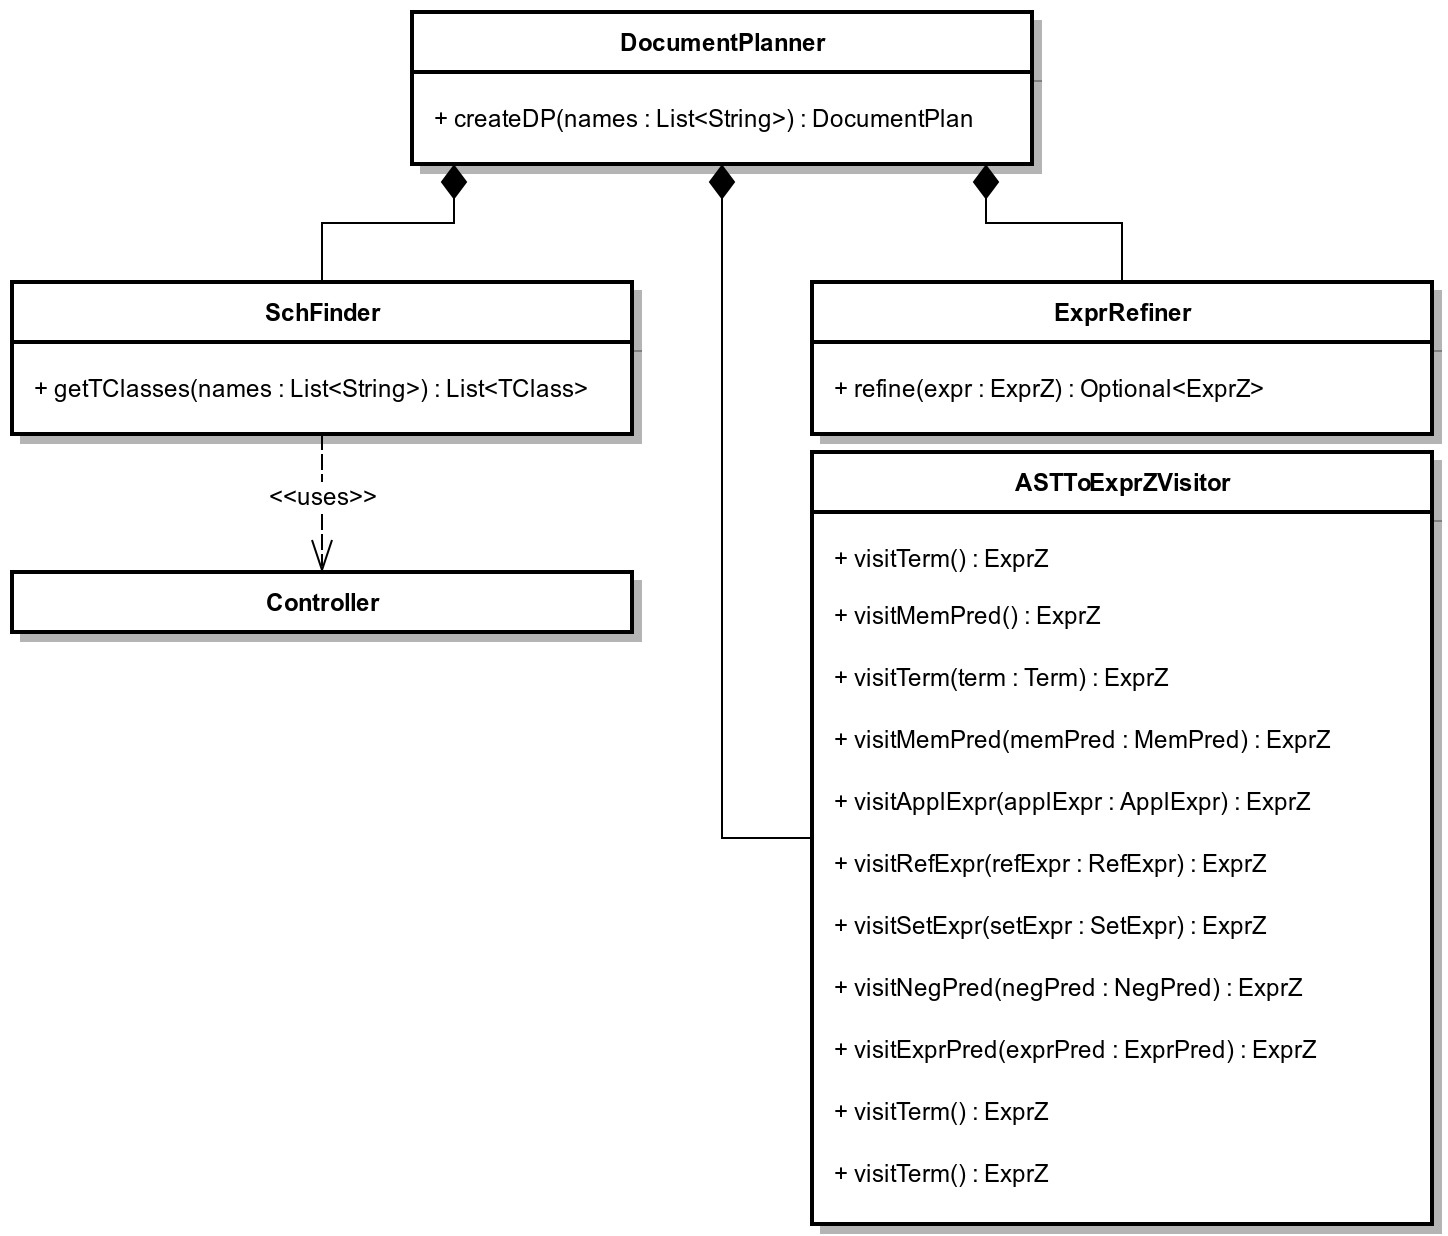
\includegraphics[scale=0.25]{img/documentplanner_imp.png}
	\caption{Diagrama clases para \textit{DocumentPlanner}}
  	\label{fig:imp_documentplanner}
\end{figure}

\bigskip
\noindent
\textbf{DocumentPlanner.} Es el módulo encargado de crear un \textit{document plan} a partir de la entrada de nuestro sistema. Construye los mensajes y estructuras intermedias de éste, delegando las tareas de determinación de contenido en los módulos que se describirán a continuación.

\bigskip
\noindent
\textbf{SchFinder.} La tarea de selección detallada en la sección \ref{cap:determinacion_contenido} será desarrollada por este módulo, que será el encargado de recuperar el conjunto de clases de prueba indicadas. El mismo posee una referencia al módulo \textit{Controller}\footnote{\textit{Controller} es el módulo encargado de mantener las referencias a elementos de la especificación, arboles de prueba, etc.} de Fastest que le permitirá identificar y recuperar las clases de prueba necesarias. 


\bigskip
\noindent
\textbf{ExprRefiner.} Es la \textit{fachada} \cite{gof} encargada de delegar los distintos procesamientos a realizar sobre las expresiones a fin de desarrollar las tareas de eliminación de tautologías y reducción de expresiones estudiadas en la sección \ref{cap:determinacion_contenido}. Podemos observar que se utilizó la clase \texttt{Optional} de Java 8 para modelar el hecho de que el método \texttt{refine()} podría no devolver un valor, por ejemplo en el caso que la expresión procesada sea una tautología y no deba ser incluida en el \textit{document plan}. En el capítulo \ref{cap:conclusion} se propone como trabajo a realizar, la implementación de nuevas tareas de razonamiento con los datos; será en esta clase en la que se deba agregar el comportamiento necesario para contemplar dichas tareas (cada una de éstas debería estar encapsulada un un módulo separado y el módulo ExprRefiner debería tener una referencia a los mismos e implementar las llamadas a los métodos de correspondientes).

\bigskip
Fastest utiliza el \textit{framework} CZT\footnote{\url{http://czt.sourceforge.net/}} que integra un conjunto de herramientas para trabajar con el lenguaje de especificación Z. La forma en la que CZT modela las expresiones de Z nos resultó compleja para este trabajo, por lo que se decidió transformar las expresiones contempladas dentro del alcance de este trabajo a un modelo más simple (lo que simplificó la implementación del algoritmo de lexicalización, por ejemplo). En la figura \ref{fig:imp_exprz} podemos observar la jerarquía de clases de las expresiones utilizadas en este trabajo para modelar las expresiones Z. 

\begin{figure}[H]
  	\centering
	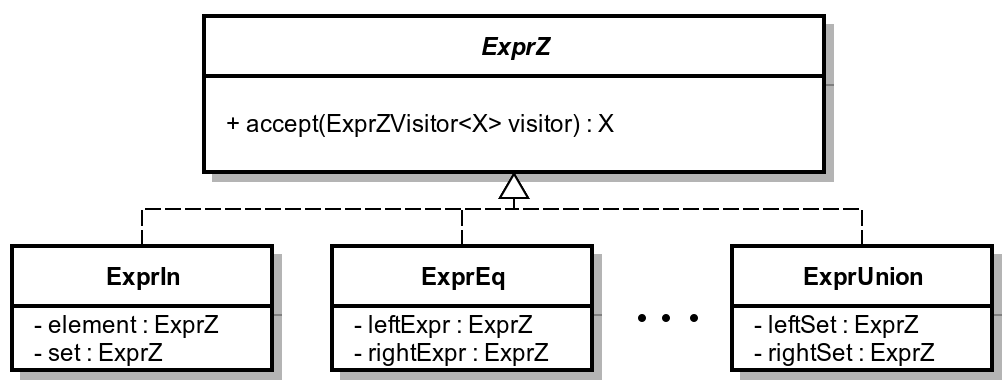
\includegraphics[scale=0.31]{img/exprz_imp.png}
	\caption{Diagrama jerarquía de clases para ExprZ}
  	\label{fig:imp_exprz}
\end{figure}

\bigskip
\noindent
\textbf{ASTToExprZVisitor.} Este módulo será el responsable de la transformación entre el modelo de CZT y el utilizado por este trabajo presentado en la figura \ref{fig:imp_exprz}.


\subsection{\textit{Microplanner}}

En esta sección se presentarán los componentes encargados de la tarea de \textit{microplanning} detallada en el capítulo \ref{cap:microplanning}. En la figura \ref{fig:imp_microplanner} podemos observar los módulos involucrados en la implementación de esta tarea.

\begin{figure}[H]
  	\centering
	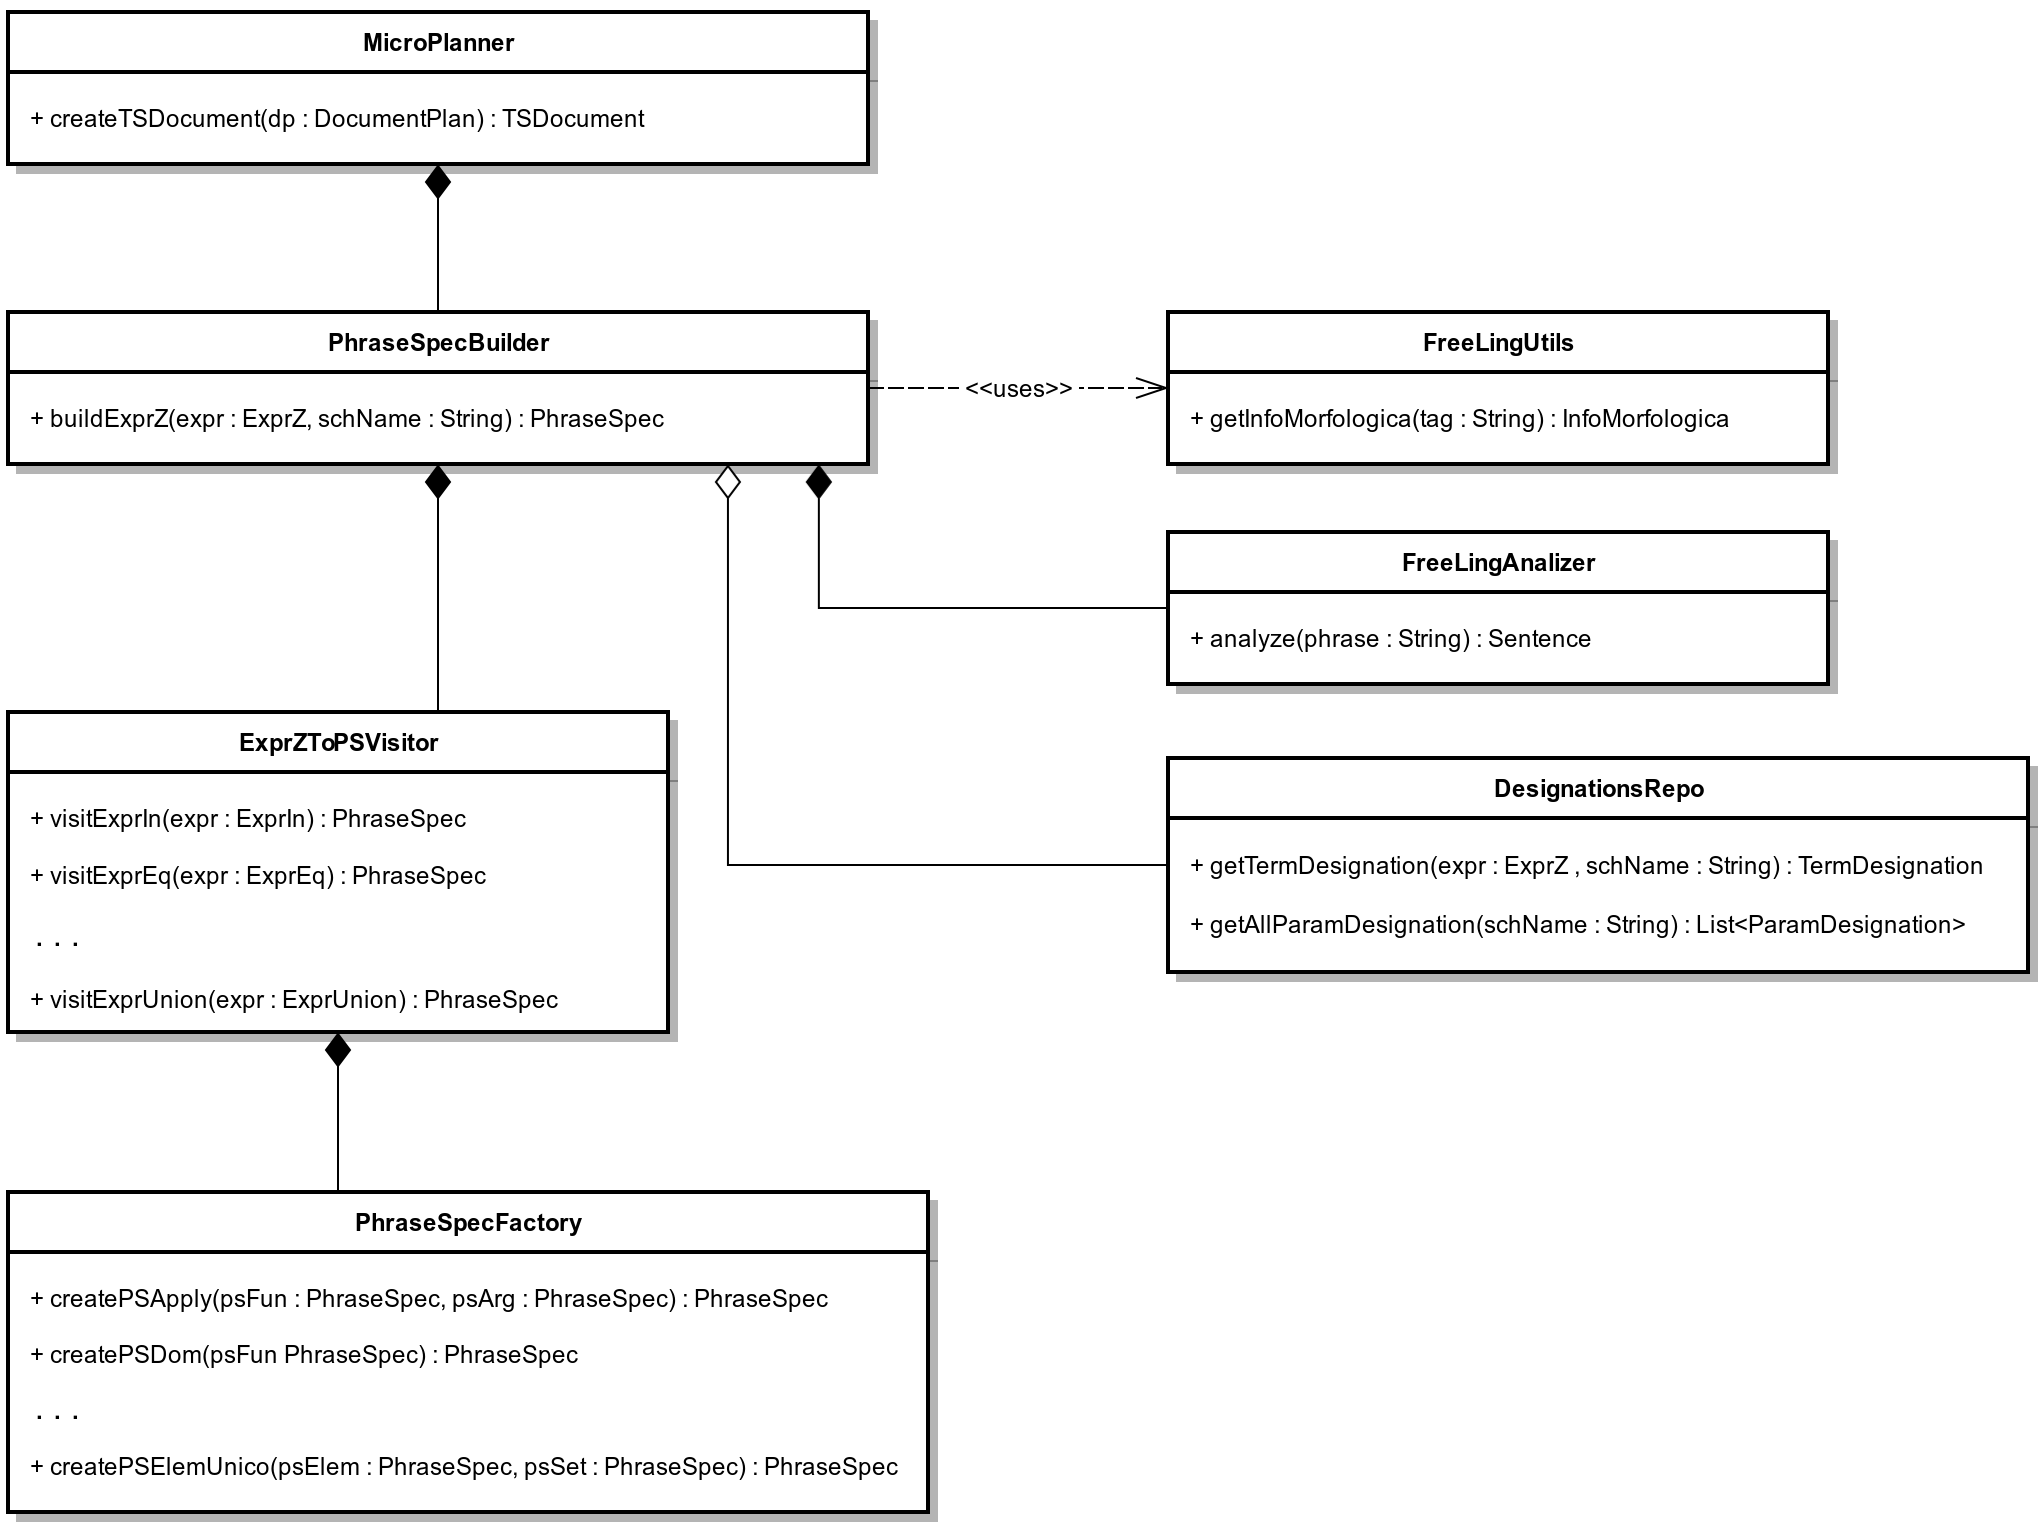
\includegraphics[scale=0.2]{img/microplanner_imp.png}
	\caption{Diagrama clases para \textit{Microplanner}}
  	\label{fig:imp_microplanner}
\end{figure}

\bigskip
\noindent
\textbf{MicroPlanner.} Es el módulo principal de esta etapa, encargado de construir la especificación del documento a partir del \textit{document plan} generado por la etapa anterior. Éste delega la tarea de lexicalización en el módulo \textit{PhraseSpecBuilder}.

\bigskip
\noindent
\textbf{PhraseSpecBuilder.} Este módulo implementa la tarea de lexicalización detallada en el capítulo \ref{cap:microplanning}, la función del mismo será construir una especificación de frase a partir de una expresión Z. Para realizar esta tarea se necesita recorrer el modelo utilizado para las expresiones Z. Se encapsuló este trabajo en el módulo \textit{ExprZToPSVisitor}, encargado del análisis de casos para las distintas expresiones y sus posibles combinaciones de acuerdo a la definición presentada en la sección \ref{sec:microplanning_lexicalization}.

\bigskip
\noindent
\textbf{ExprZToPSVisitor.} Encapsula las reglas de lexicalización para todas las posibles expresiones y combinaciones de las mismas. Implementa la función auxiliar \textsc{lexicalización'()} utilizada en el bosquejo del algoritmo \ref{fig:algoritmo_lexicalizacion}. Se utilizó el patrón de diseño \textit{visitor} \cite{gof} para iterar sobre la estructura de las distintas expresiones Z modeladas por nuestro sistema.

\bigskip
\noindent
\textbf{PhraseSpecFactory.} Construir y componer las especificaciones de frase de nuestro sistema resulta una tarea relativamente compleja. Es por esto que se encapsuló esta funcionalidad en el módulo \textit{PhraseSpecFactory} encargado de construir apropiadamente las distintas especificaciones de frase de nuestro sistema. Por ejemplo: \texttt{createPSElemUnico()} tomará dos especificaciones de frase y las compondrá para generar una nueva especificación para la frase \textit{``... es el único elemento de ...''}, siendo las dos especificaciones mencionadas anteriormente las encargadas de modelar el texto que precede y antecede respectivamente a la anterior.

\bigskip
\noindent
\textbf{FreeLingAnalizer.} Se utilizó el analizador morfosintáctico \textit{FreeLing} para obtener las características morfológicas de los distintos constituyentes de las frases utilizadas en las designaciones. Este módulo tendrá la tarea de interactuar con las librerías provistas por la herramienta proveyéndonos de la información necesaria (como el núcleo de la frase, su género, número, etc.) para poder construir una especificación de frase a partir de una designación.

\bigskip
\noindent
\textbf{FreeLingUtils.} Contiene algunos métodos útiles para el trabajo con \textit{FreeLing}. Por ejemplo, \textit{FreeLing} genera una estructura en la que etiqueta cada palabra con anotaciones morfosintácticas. El método \texttt{getInfoMorfologica()} procesa estas anotaciones produciendo una estructura más sencilla con la que trabajará nuestro sistema.

\bigskip
\noindent
\textbf{DesignationsRepo.} Es necesario para el algoritmo de lexicalización saber si una expresión se encuentra designada y, en ese caso, necesitará saber cuál es su designación. Será a través de este módulo que podrá acceder a las designaciones presentes en la especificación. El mismo se inicializa al cargar la especificación en Fastest. 

%TODO cambiar nombres a español
\subsection{\textit{Surface Realizer}}

Finalmente, el módulo \emph{SurfaceRealizer} será el encargado de generar el texto de superficie para el documento final en base a una especificación del mismo. En esta etapa se realizan las tareas de realización estructural y lingüística presentadas en el capítulo \ref{cap:realization}. En la figura \ref{fig:imp_surfrealizer} podemos ver los componentes más relevantes involucrados en esta etapa, cuya función se describirá a continuación. 

\begin{figure}[H]
  	\centering
	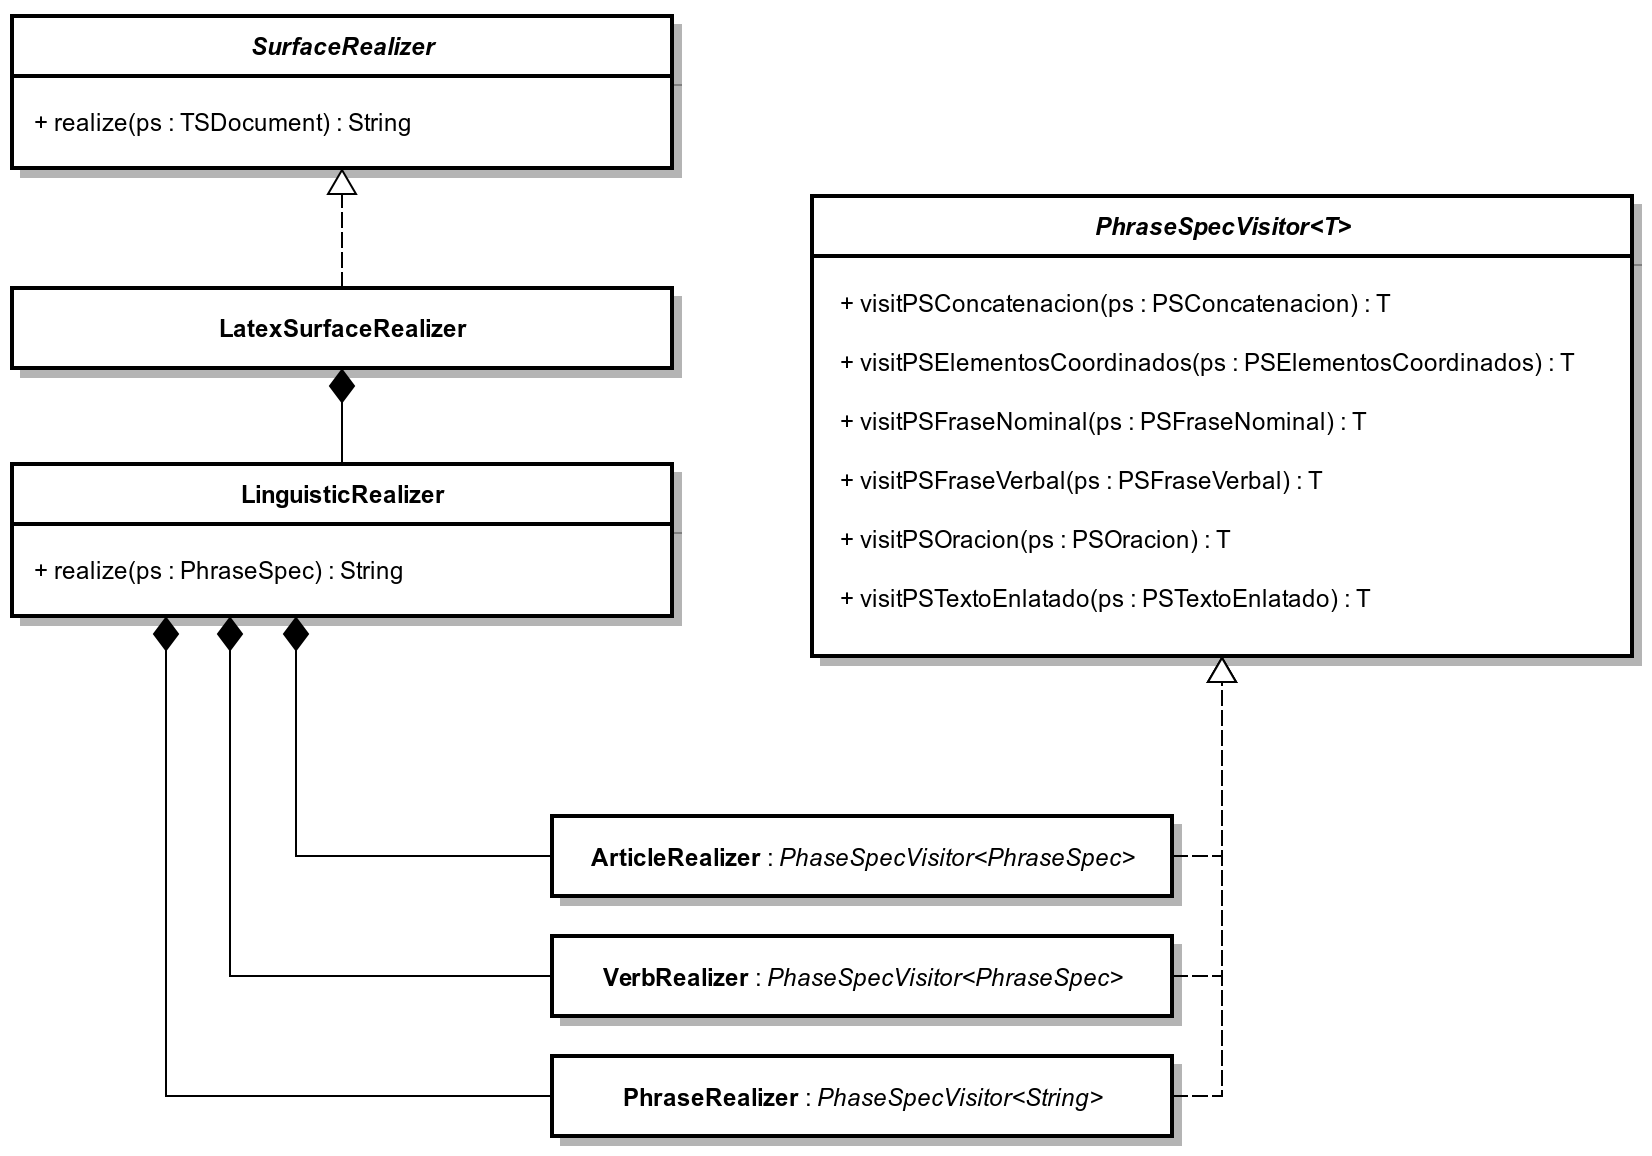
\includegraphics[scale=0.20]{img/realizer_imp.png}
	\caption{Diagrama clases para \textit{Surface Realizer}}
  	\label{fig:imp_surfrealizer}
\end{figure}

\bigskip
\noindent
\textbf{SurfaceRealizer.} Como se mencionó en la sección \ref{cap:realization} la tarea de realización estructural resulta dependiente del sistema de presentación utilizado. Es por esto que se definió la interfaz abstracta \textit{SurfaceRealizer} y una implementación especifica encargada de producir código \LaTeX~apropiado para el documento final. El método principal de esta clase toma una especificación del documento final y tiene la misión de producir el texto en lenguaje natural esperado, para esto deberá hacer uso del \textit{LinguisticRealizer} para lograr la realización lingüística de cada una de las especificaciones de frase presentes en la especificación de documento dada. 


\bigskip
\noindent
\textbf{LinguisticRealizer.} Es el módulo encargado de la realización lingüística. Es responsabilidad de este módulo asegurarse de que las frases del texto generado respeten las reglas gramaticales introducidas en el capítulo \ref{cap:linguistic_realization}. Éste hace uso de los módulos \textit{ArticleRealizer} y \textit{VerbRealizer} para resolver las cuestiones de concordancia gramatical, delegando la generación del texto final en el módulo \textit{PhraseRealizer}. 

\bigskip
\noindent
\textbf{PhraseSpecVisitor.} Se utilizó el patrón \textit{visitor} para iterar sobre la estructura de las especificaciones de frase. A continuación veremos la función de las tres implementaciones más importantes de esta interfaz. 

\bigskip
\noindent
\textbf{ArticleRealizer.} Es el módulo encargado de recorrer la estructura de una especificación de frase y escoger el artículo apropiado (de ser necesario en una frase nominal) de forma tal que concuerde según las reglas gramaticales introducidas previamente. El artículo será agregado sobre la misma estructura utilizada para la especificación de frase.

\bigskip
\noindent
\textbf{VerbRealizer.} Este módulo tiene la responsabilidad de conjugar el verbo de una oración (establecido en infinitivo por el \textit{microplanner}) y escoger el atributo apropiado en caso de ser un verbo copulativo, teniendo en cuenta los aspectos gramaticales detallados en la sección \ref{cap:linguistic_realization}. Al igual que con \textit{ArticleRealizer}, se reutilizó la estructura utilizada para la especificación de frases para establecer el verbo correcto y atributo (reemplazando el verbo infinitivo por el verbo correctamente conjugado y el atributo previamente establecido por el atributo correspondiente).

\bigskip
\noindent
\textbf{PhraseRealizer.} Será el módulo finalmente encargado de recorrer la estructura de una especificación de frase y generar el texto final correspondiente a la misma. En esta etapa casi todo el trabajo fue realizado. La función de este módulo será extraer el texto contenido en la especificación de frase con el fin de generar la frase final respetando el orden establecido e introduciendo los espacios y signos de puntuación necesarios. Es importante aclarar que resulta necesario que se ejecuten en primer instancia las tareas realizadas por \textit{PhraseSpecVisitor} y \textit{VerbRealizer} ya que \textit{PhraseRealizer} asumirá que ya fueron resueltos previamente todos los aspectos gramaticales.

\section{Resumen del capítulo}
En este capítulo se presentó el prototipo desarrollado como resultado de este trabajo. Se mostró su integración con Fastest, presentando los nuevos comandos introducidos para la generación de descripciones de clases de prueba y describiendo su modo de uso. Se detalló también la forma en la que el especificador debe escribir las designaciones para que el sistema pueda hacer uso de ellas. Finalmente se comentaron los aspectos más interesantes de la implementación realizada junto con algunas recomendaciones para futuras modificaciones.
\include{sec/evaluacion}
\chapter{Conclusiones y trabajo futuro}
\label{cap:conclusion}

\section*{Conclusión}
En este trabajo hemos presentado y desarrollado una solución para la generación automática de descripciones en lenguaje natural para clases de prueba generadas por el TTF. Para esto, fue necesario utilizar técnicas de generación de lenguaje natural. En particular, seguimos la metodología propuesta por Reiter y Dale \cite{reiter_dale}.

En primer instancia recolectamos y analizamos un corpus con textos de ejemplo. A partir de éste extrajimos los requerimientos más importantes para el desarrollo de nuestro sistema. Luego, estudiamos en detalle las tareas mas importantes que debían ser llevadas a cabo por nuestro sistema. En el capítulo \ref{cap:document_planning} hicimos especial incapie en la determinación de contenido y cómo el razonamiento con los datos puede mejorar notablemente la calidad de las descripciones generadas por nuestro sistema. En el capítulo \ref{cap:microplanning} utilizamos el conjunto de reglas de traducción obtenido como resultado del análisis del corpus para definir la tarea de lexicalización de expresiones Z, encargada de escoger que palabras y constructores sintácticos utilizar para comunicar la información requerida. Estudiamos además, el importante rol que cumplen las designaciones para este trabajo y como nuestra tarea de lexicalización hace uso de la información contenida en las mismas. Por último, en el capítulo \ref{cap:realization} nos encargamos fundamentalmente de estudiar los aspectos necesarios para, finalmente, generar texto sintáctica, ortográfica y gramaticalmente correcto.

Como resultado de este trabajo, hemos implementado un prototipo en base al desarrollo realizado. Utilizando para esto un diseño flexible capaz de admitir futuras posibilidades de evolución. 

El sistema desarrollado trabaja principalmente con la información contenida en las clases de prueba, haciendo un especial uso de las designaciones que acompañan a la especificación. Estas designaciones resultan una fuente fundamental de información que le permite a nuestro sistema generar las porciones de texto dependientes del dominio de aplicación y de esta forma lograr una generación de descripciones en lenguaje natural independiente del dominio de aplicación y de la cantidad de clases y casos de pruebas.

\section*{Trabajo futuro}

Consideramos que el trabajo realizado esta abierto a nuevos aportes. A continuación detallaremos algunos de los aportes que creemos que podrían realizarse como trabajo futuro.

El sistema desarrollado no cubre la totalidad de las expresiones y operadores de Z; dentro del alcance de este trabajo establecimos un subconjunto de éstas con las que trabajamos. Un aporte interesante podría ser la extensión de expresiones soportadas por nuestro sistema. Para esto debería expandirse el corpus, contemplando casos para los operadores a introducir y luego volver a realizar un análisis del mismo extrayendo nuevas reglas para describir los mismos. 

Por otro lado, creemos que es posible profundizar el trabajo sobre los datos de entrada e incluir nuevas tareas de razonamiento sobre los mismos en la etapa de \textit{document planning}. Esto le permitiría a nuestro sistema mejorar la calidad de los textos producidos. Por ejemplo, se podría trabajar sobre las expresiones redundantes que pueden aparecer en una clase de prueba.

Como mencionamos en el capítulo \ref{cap:microplanning} nuestro sistema no realiza tareas de agregación y generación de expresiones de referencia. Podría resultar interesante introducir tareas de este tipo a nuestro sistema.

El sistema desarrollado actualmente es capaz de producir únicamente textos en castellano. Un aporte importante podría ser expandir el mismo para que éste contemple la generación de textos en otras lenguas, por ejemplo en inglés. Para generar textos en inglés por ejemplo, existen realizadores lingüísticos de código abierto que podríamos utilizar para ayudarnos en este desarrollo; en este caso tendríamos que implementar un nuevo módulo de \textit{microplanning} de modo que sea capaz de generar las estructuras utilizadas por el realizador lingüístico a utilizar.
\appendix
\chapter{Corpus de descripciones}
\label{ape:corpus}

Para construir el corpus utilizado para este trabajo utilizamos 5 especificaciones de distintos dominios de aplicación con sus respectivos casos y clases de prueba generados por Fastest. De estas clases de prueba escogimos las más interesantes para traducir acabando con un total de 98 clases de prueba.

A continuación presentaremos 3 de los ejemplos recolectados que forman parte del corpus utilizado y resultan representativos del total de ejemplos recolectados. En éstos incluimos tanto la especificación utilizada para generar las clases de prueba a traducir, como también las designaciones necesarias para poder describir las clases de prueba seleccionadas y las descripciones de las mismas.

\section*{Ejemplo: \textit{Symbol Table}}

\subsection*{Especificación y designaciones}

\begin{zed}
[SYM, VAL] \also
REPORT ::= ok | symbolNotPresent
\end{zed}

\begin{itemize}
  \item Tabla de símbolos $\approx st$ \\
  \item Símbolos cargados en la tabla $\approx dom~st$ \\
  \item Valor de $x$ $\approx st~x$ 
\end{itemize}

\begin{schema}{ST}
st: SYM \pfun VAL
\end{schema}

\begin{itemize}
  \item Intenta actualizar el valor de un símbolo $\approx Update$ \\
  \item Símbolo a actualizar $\approx s?$ \\
  \item Valor a actualizar  $\approx v?$ 
\end{itemize}

\begin{schema}{Update}
\Delta ST \\
s?: SYM \\
v?: VAL \\
rep!: REPORT
\where
st' = st \oplus \{s? \mapsto v?\} \\
rep! = ok
\end{schema}

\begin{itemize}
  \item Símbolo a buscar $\approx s?$ \\
  \item Valor del símbolo buscado  $\approx v?$ 
\end{itemize}

\begin{schema}{LookUpOk}
\Xi ST \\
s?: SYM \\
v!: VAL \\
rep!: REPORT
\where
s? \in \dom st \\
v! = st~s? \\
rep! = ok
\end{schema}

\begin{schema}{LookUpE}
\Xi ST \\
s?: SYM \\
rep!: REPORT
\where
s? \notin \dom st \\
rep! = symbolNotPresent
\end{schema}

\begin{itemize}
  \item Intenta buscar el valor de un símbolo $\approx LookUp$ 
\end{itemize}

\begin{zed}
LookUp == LookUpOk \lor LookUpE
\end{zed}

\begin{itemize}
  \item Símbolo a eliminar $\approx s?$ 
\end{itemize}

\begin{schema}{DeleteOk}
\Delta ST \\
s?: SYM \\
rep!: REPORT
\where
s? \in \dom st \\
st' = \{s?\} \ndres st \\
rep! = ok
\end{schema}

\begin{itemize}
  \item Intenta eliminar un símbolo de la tabla $\approx Delete$ 
\end{itemize}

\begin{zed}
DeleteE == LookUpE \also
Delete == DeleteOk \lor DeleteE
\end{zed}

\subsection*{Clases de prueba y descripciones}

\begin{schema}{LookUp\_ SP\_ 1}\\
 st : SYM \pfun VAL \\
 s? : SYM 
\where
 s? \in \dom st \\
 \dom st = \{ s? \}
\end{schema}

\begin{tcolorbox}[colback=gray!5!white,colframe=gray!50!black,
  colbacktitle=gray!75!black,title=LookUp\_ SP\_ 1]
  Se intenta buscar el valor de un símbolo, cuando:
     \begin{itemize}
        \item[--]{El símbolo a buscar pertenece a los símbolos cargados en la tabla.}
        \item[--]{El símbolo a buscar es el único elemento de los símbolos cargados en la tabla.}
     \end{itemize}
\end{tcolorbox}
%TODO aca se podria eliminar la primera restriccion

\begin{schema}{LookUp\_ SP\_ 4}\\
 st : SYM \pfun VAL \\
 s? : SYM 
\where
 s? \notin \dom st \\
 \dom st \neq \{ s? \} \\
 s? \in \dom st
\end{schema}

\begin{tcolorbox}[colback=gray!5!white,colframe=gray!50!black,
  colbacktitle=gray!75!black,title=LookUp\_ SP\_ 4]
  Se intenta buscar el valor de un símbolo, cuando:
     \begin{itemize}
        \item[--]{El símbolo a buscar no pertenece a los símbolos cargados en la tabla.}
        \item[--]{Los símbolos cargados en la tabla no son iguales al conjunto formado por el símbolo a buscar.}
        \item[--]{El símbolo a buscar pertenece a los símbolos cargados en la tabla.}
     \end{itemize}
\end{tcolorbox}

\begin{schema}{Update\_ SP\_ 1}\\
 st : SYM \pfun VAL \\
 s? : SYM \\
 v? : VAL 
\where
 st = \{ \} \\
 \{ s? \mapsto v? \} = \{ \}
\end{schema}

\begin{tcolorbox}[colback=gray!5!white,colframe=gray!50!black,
  colbacktitle=gray!75!black,title=Update\_ SP\_ 1]
  Se intenta actualizar el valor de un símbolo, cuando:
     \begin{itemize}
        \item[--]{No hay ningún elemento en la tabla de símbolos.}
        \item[--]{No hay elementos en el conjunto formado por el par ordenado por: el símbolo a actualizar y el valor a actualizar.}
      \end{itemize}
\end{tcolorbox}


\begin{schema}{Update\_ SP\_ 2}\\
 st : SYM \pfun VAL \\
 s? : SYM \\
 v? : VAL 
\where
 st = \{ \} \\
 \{ s? \mapsto v? \} \neq \{ \}
\end{schema}

\begin{tcolorbox}[colback=gray!5!white,colframe=gray!50!black,
  colbacktitle=gray!75!black,title=Update\_ SP\_ 2]
  Se intenta actualizar el valor de un símbolo, cuando:
     \begin{itemize}
        \item[--]{No hay ningún elemento en la tabla de símbolos.}
        \item[--]{Existe al menos un elemento en el conjunto formado por el par ordenado por: el símbolo a actualizar y el valor a actualizar.}
     \end{itemize}
\end{tcolorbox}


\begin{schema}{Update\_ SP\_ 3}\\
 st : SYM \pfun VAL \\
 s? : SYM \\
 v? : VAL 
\where
 st \neq \{ \} \\
 \{ s? \mapsto v? \} = \{ \}
\end{schema}

\begin{tcolorbox}[colback=gray!5!white,colframe=gray!50!black,
  colbacktitle=gray!75!black,title=Update\_ SP\_ 3]
  Se intenta actualizar el valor de un símbolo, cuando:
     \begin{itemize}
        \item[--]{Existe al menos un elemento en la tabla de símbolos.}
        \item[--]{No hay elementos en el conjunto formado por el par ordenado por: el símbolo a actualizar y el valor a actualizar.}
     \end{itemize}
\end{tcolorbox}


\begin{schema}{Update\_ SP\_ 4}\\
 st : SYM \pfun VAL \\
 s? : SYM \\
 v? : VAL 
\where
 st \neq \{ \} \\
 \{ s? \mapsto v? \} \neq \{ \} \\
 \dom st = \dom \{ s? \mapsto v? \}
\end{schema}

\begin{tcolorbox}[colback=gray!5!white,colframe=gray!50!black,
  colbacktitle=gray!75!black,title=Update\_ SP\_ 4]
  Se intenta actualizar el valor de un símbolo, cuando:
     \begin{itemize}
        \item[--]{Existe al menos un elemento en la tabla de símbolos.}
        \item[--]{Existe al menos un elemento en el conjunto formado por el par ordenado por: el símbolo a actualizar y el valor a actualizar.}
        \item[--]{El símbolo a actualizar pertenece a los símbolos cargados en la tabla.}
     \end{itemize}
\end{tcolorbox}

\begin{schema}{Update\_ SP\_ 5}\\
 st : SYM \pfun VAL \\
 s? : SYM \\
 v? : VAL 
\where
 st \neq \{ \} \\
 \{ s? \mapsto v? \} \neq \{ \} \\
 \dom \{ s? \mapsto v? \} \subset \dom st
\end{schema}

\begin{tcolorbox}[colback=gray!5!white,colframe=gray!50!black,
  colbacktitle=gray!75!black,title=Update\_ SP\_ 5]
  Se intenta actualizar el valor de un símbolo, cuando:
     \begin{itemize}
        \item[--]{Existe al menos un elemento en la tabla de símbolos.}
        \item[--]{Existe al menos un elemento en el conjunto formado por el par ordenado por: el símbolo a actualizar y el valor a actualizar.}
        \item[--]{El símbolo a actualizar es el único elemento de los símbolos cargados en la tabla.}
     \end{itemize}
\end{tcolorbox}


\begin{schema}{Update\_ SP\_ 6}\\
 st : SYM \pfun VAL \\
 s? : SYM \\
 v? : VAL 
\where
 st \neq \{ \} \\
 \{ s? \mapsto v? \} \neq \{ \} \\
 ( \dom st \cap \dom \{ s? \mapsto v? \} ) = \{ \}
\end{schema}

\begin{tcolorbox}[colback=gray!5!white,colframe=gray!50!black,
  colbacktitle=gray!75!black,title=Update\_ SP\_ 6]
  Se intenta actualizar el valor de un símbolo, cuando:
     \begin{itemize}
        \item[--]{Existe al menos un elemento en la tabla de símbolos.}
        \item[--]{Existe al menos un elemento en el conjunto formado por el par ordenado por: el símbolo a actualizar y el valor a actualizar.}
        \item[--]{Los símbolos cargados en la tabla están incluidos en el conjunto formado por el símbolo a actualizar.}
     \end{itemize}
\end{tcolorbox}


\begin{schema}{Delete\_ SP\_ 2}\\
 st : SYM \pfun VAL \\
 s? : SYM 
\where
 s? \in \dom st \\
 st \neq \{ \} \\
 \{ s? \} = \{ \}
\end{schema}

\begin{tcolorbox}[colback=gray!5!white,colframe=gray!50!black,
  colbacktitle=gray!75!black,title=Delete\_ SP\_ 2]
  Se intenta eliminar un símbolo de la tabla, cuando:
     \begin{itemize}
        \item[--]{El símbolo a eliminar pertenece a los símbolos cargados en la tabla.}
        \item[--]{Existe al menos un elemento en la tabla de símbolos.}
        \item[--]{No hay ningún elemento en el conjunto formado por: el símbolo a eliminar.}
     \end{itemize}
\end{tcolorbox}


\begin{schema}{Delete\_ SP\_ 3}\\
 st : SYM \pfun VAL \\
 s? : SYM 
\where
 s? \in \dom st \\
 st \neq \{ \} \\
 \{ s? \} = \dom st
\end{schema}

\begin{tcolorbox}[colback=gray!5!white,colframe=gray!50!black,
  colbacktitle=gray!75!black,title=Delete\_ SP\_ 3]
  Se intenta eliminar un símbolo de la tabla, cuando:
     \begin{itemize}
        \item[--]{El símbolo a eliminar pertenece a los símbolos cargados en la tabla.}
        \item[--]{Existe al menos un elemento en la tabla de símbolos.}
        \item[--]{El símbolo a eliminar es el único elemento de los símbolos cargados en la tabla.}
     \end{itemize}
\end{tcolorbox}


\begin{schema}{Delete\_ SP\_ 4}\\
 st : SYM \pfun VAL \\
 s? : SYM 
\where
 s? \in \dom st \\
 st \neq \{ \} \\
 \{ s? \} \neq \{ \} \\
 \{ s? \} \subset \dom st
\end{schema}

\begin{tcolorbox}[colback=gray!5!white,colframe=gray!50!black,
  colbacktitle=gray!75!black,title=Delete\_ SP\_ 4]
  Se intenta eliminar un símbolo de la tabla, cuando:
     \begin{itemize}
        \item[--]{El símbolo a eliminar pertenece los símbolos cargados en la tabla.}
        \item[--]{Existe al menos un elemento en la tabla de símbolos.}
        \item[--]{Existe al menos un elemento en el conjunto formado por: el símbolo a eliminar.}
        \item[--]{El símbolo a eliminar pertenece los símbolos cargados en la tabla.}
     \end{itemize}
\end{tcolorbox}


\begin{schema}{Delete\_ SP\_ 5}\\
 st : SYM \pfun VAL \\
 s? : SYM 
\where
 s? \in \dom st \\
 st \neq \{ \} \\
 \{ s? \} \neq \{ \} \\
 \{ s? \} \cap \dom st = \{ \}
\end{schema}

\begin{tcolorbox}[colback=gray!5!white,colframe=gray!50!black,
  colbacktitle=gray!75!black,title=Delete\_ SP\_ 5]
  Se intenta eliminar un símbolo de la tabla, cuando:
     \begin{itemize}
        \item[--]{El símbolo a eliminar pertenece los símbolos cargados en la tabla.}
        \item[--]{Existe al menos un elemento en la tabla de símbolos.}
        \item[--]{Existe al menos un elemento en el conjunto formado por: el símbolo a eliminar.}
        \item[--]{El conjunto formado por el símbolo a eliminar y los símbolos cargados en la tabla no tienen ningún elemento en común.}
     \end{itemize}
\end{tcolorbox}


\begin{schema}{Delete\_ SP\_ 7}\\
 st : SYM \pfun VAL \\
 s? : SYM 
\where
 s? \in \dom st \\
 st \neq \{ \} \\
 \{ s? \} \cap \dom st \neq \{ \} \\
 \lnot \dom st \subseteq \{ s? \} \\
 \lnot \{ s? \} \subseteq \dom st
\end{schema}

\begin{tcolorbox}[colback=gray!5!white,colframe=gray!50!black,
  colbacktitle=gray!75!black,title=Delete\_ SP\_ 7]
  Se intenta eliminar un símbolo de la tabla, cuando:
     \begin{itemize}
        \item[--]{El símbolo a eliminar pertenece los símbolos cargados en la tabla.}
        \item[--]{Existe al menos un elemento en la tabla de símbolos.}
        \item[--]{El conjunto formado por el símbolo a eliminar y los símbolos cargados en la tabla tienen tienen al menos un elemento en común.}
        \item[--]{Existe al menos un elemento en los símbolos cargados en la tabla que no pertenece al conjunto formado por: el símbolo a eliminar.}
        \item[--]{El símbolo a eliminar no pertenece al los símbolos cargados en la tabla.}
     \end{itemize}
\end{tcolorbox}


\begin{schema}{Delete\_ SP\_ 12}\\
 st : SYM \pfun VAL \\
 s? : SYM 
\where
 s? \notin \dom st \\
 st \neq \{ \} \\
 \{ s? \} \neq \{ \} \\
 \{ s? \} \cap \dom st = \{ \}
\end{schema}

\begin{tcolorbox}[colback=gray!5!white,colframe=gray!50!black,
  colbacktitle=gray!75!black,title=Delete\_ SP\_ 12]
  Se intenta eliminar un símbolo de la tabla, cuando:
     \begin{itemize}
        \item[--]{El símbolo a eliminar no pertenece los símbolos cargados en la tabla.}
        \item[--]{Existe al menos un elemento en la tabla de símbolos.}
        \item[--]{Existe al menos un elemento en el conjunto formado por: el símbolo a eliminar.}
        \item[--]{El conjunto formado por el símbolo a eliminar y los símbolos cargados en la tabla no tienen ningún elemento en común.}
     \end{itemize}
\end{tcolorbox}


\begin{schema}{Delete\_ SP\_ 13}\\
 st : SYM \pfun VAL \\
 s? : SYM 
\where
 s? \notin \dom st \\
 st \neq \{ \} \\
 \{ s? \} \cap \dom st \neq \{ \} \\
 \dom st \subset \{ s? \}
\end{schema}

\begin{tcolorbox}[colback=gray!5!white,colframe=gray!50!black,
  colbacktitle=gray!75!black,title=Delete\_ SP\_ 13]
  Se intenta eliminar un símbolo de la tabla, cuando:
     \begin{itemize}
        \item[--]{El símbolo a eliminar no pertenece los símbolos cargados en la tabla.}
        \item[--]{Existe al menos un elemento en la tabla de símbolos.}
        \item[--]{El conjunto formado por el símbolo a eliminar y los símbolos cargados en la tabla tienen tienen al menos un elemento en común.}
        \item[--]{Los símbolos cargados en la tabla están incluidos en el conjunto formado por: el símbolo a eliminar.}
     \end{itemize}
\end{tcolorbox}

\section*{Ejemplo: Banco}

\subsection*{Especificación y designaciones}

\begin{zed}
[NCTA] \also

SALDO == \nat \also

MENSAJES ::= ok | numeroClienteEnUso | noPoseeSaldoSuficiente | saldoNoNulo
\end{zed}

\begin{itemize}
  \item Cajas de ahorro existentes en el banco $\approx cajas$ \\
  \item Números de cuenta cargados en el banco $\approx dom~cajas$ \\
  \item Dinero depositado en la caja de ahorro de $x$ $\approx caja~x$ 
\end{itemize}

\begin{schema}{Banco}
cajas: NCTA \pfun SALDO
\end{schema}

\begin{itemize}
  \item Número de cuenta del cliente $\approx num?$ 
\end{itemize}

\begin{schema}{DepositarOk}
\Delta Banco \\
num?: NCTA; m?: \num
\where
num? \in \dom cajas \\
m? > 0 \\
cajas' = cajas \oplus \{num? \mapsto cajas~num? + m?\}
\end{schema}

\begin{zed}
DepositarE1 == [\Xi Banco; num?:NCTA | num? \notin \dom cajas]
\end{zed}

\begin{zed}
DepositarE2 == [\Xi Banco; m?: \num | m? \leq 0]
\end{zed}

\begin{itemize}
  \item Intenta depositar dinero en una cuenta $\approx Depositar$ 
\end{itemize}

\begin{zed}
Depositar == DepositarOk \lor DepositarE1 \lor DepositarE2
\end{zed}

\begin{itemize}
  \item Número de cuenta del nuevo cliente $\approx num?$ 
\end{itemize}

\begin{schema}{NuevoClienteOk}
\Delta Banco \\
num?:NCTA \\
rep!:MENSAJES
\where
num? \notin \dom cajas \\
cajas' = cajas \cup \{num? \mapsto 0\} \\
rep! = ok
\end{schema}

\begin{schema}{NuevoClienteE}

\Xi Banco \\
num?:NCTA \\
rep!:MENSAJES
\where
num? \in \dom cajas \\
rep! = numeroClienteEnUso
\end{schema}

\begin{itemize}
  \item Intenta cargar un nuevo cliente $\approx NuevoCliente$ 
\end{itemize}

\begin{zed}
NuevoCliente == NuevoClienteOk \lor NuevoClienteE
\end{zed}

\begin{itemize}
  \item Número de cuenta del cliente $\approx num?$ 
\end{itemize}

\begin{schema}{ExtraerOk}
\Delta Banco \\
num?:NCTA \\
m?:SALDO \\
rep!:MENSAJES
\where
num? \in \dom cajas \\
0 < m? \\
m? \leq cajas~num? \\
cajas' = cajas \oplus \{num? \mapsto (cajas~num?) - m?\} \\
rep! = ok
\end{schema}

\begin{zed}
ExtraerE1 == DepositarE1 \also

ExtraerE2 == DepositarE2
\end{zed}

\begin{schema}{ExtraerE3}
\Xi Banco \\
num?:NCTA \\
m?:SALDO \\
rep!:MENSAJES
\where
m? > cajas~num? \\
num? \in \dom cajas \\
rep! = noPoseeSaldoSuficiente
\end{schema}

\begin{itemize}
  \item Intenta realizar una extracción de dinero $\approx Extraer$ 
\end{itemize}

\begin{zed}
ExtraerE == ExtraerE1 \lor ExtraerE2 \lor ExtraerE3 \also

Extraer == ExtraerOk \lor ExtraerE
\end{zed}

\begin{itemize}
  \item Número de cuenta del cliente $\approx num$ 
\end{itemize}

\begin{schema}{PedirSaldoOk}
\Xi Banco \\
num?:NCTA \\
saldo!:SALDO \\
rep!:MENSAJES
\where
num? \in \dom cajas \\
saldo! = cajas~num? \\
rep! = ok
\end{schema}

\begin{itemize}
  \item Intenta consultar el saldo de un cliente $\approx PedirSaldo$ 
\end{itemize}

\begin{zed}
PedirSaldoE == DepositarE1 \also

PedirSaldo == PedirSaldoOk \lor PedirSaldoE
\end{zed}

\subsection*{Clases de prueba y descripciones}

\begin{schema}{NuevoCliente\_ SP\_ 2}\\
 cajas : NCTA \pfun SALDO \\
 num? : NCTA 
\where
 num? \notin \dom cajas \\
 cajas = \{ \} \\
 \{ num? \mapsto 0 \} \neq \{ \}
\end{schema}

\begin{tcolorbox}[colback=gray!5!white,colframe=gray!50!black,
  colbacktitle=gray!75!black,title=NuevoCliente\_SP\_2]
  Se intenta cargar un nuevo cliente, cuando:
     \begin{itemize}
        \item[--]{El número de cuenta del nuevo cliente no pertenece a los números de cuenta cargados en el banco.}
        \item[--]{No hay ningún elemento en las cajas de ahorro existentes en el banco.}
        \item[--]{Existe al menos un elemento en el conjunto formado por el par: número de cuenta y 0.}
     \end{itemize}
\end{tcolorbox}


\begin{schema}{NuevoCliente\_ SP\_ 4}\\
 cajas : NCTA \pfun SALDO \\
 num? : NCTA 
\where
 num? \notin \dom cajas \\
 cajas \neq \{ \} \\
 \{ num? \mapsto 0 \} \neq \{ \} \\
 \dom cajas = \dom \{ num? \mapsto 0 \}
\end{schema}

\begin{tcolorbox}[colback=gray!5!white,colframe=gray!50!black,
  colbacktitle=gray!75!black,title=NuevoCliente\_SP\_4]
  Se intenta cargar un nuevo cliente, cuando:
     \begin{itemize}
        \item[--]{El número de cuenta del nuevo cliente no pertenece a los números de cuenta cargados en el banco.}
        \item[--]{Existe al menos un elemento en las cajas de ahorro existentes en el banco.}
        \item[--]{Existe al menos un elemento en el conjunto formado pope el par: número de cuenta y 0.}
        \item[--]{El número de cuenta del nuevo cliente es el único elemento de los números de cuenta cargados en el banco.}
     \end{itemize}
\end{tcolorbox}


\begin{schema}{NuevoCliente\_ SP\_ 5}\\
 cajas : NCTA \pfun SALDO \\
 num? : NCTA 
\where
 num? \notin \dom cajas \\
 cajas \neq \{ \} \\
 \{ num? \mapsto 0 \} \neq \{ \} \\
 \dom \{ num? \mapsto 0 \} \subset \dom cajas
\end{schema}

\begin{tcolorbox}[colback=gray!5!white,colframe=gray!50!black,
  colbacktitle=gray!75!black,title=NuevoCliente\_SP\_5]
  Se intenta cargar un nuevo cliente, cuando:
     \begin{itemize}
        \item[--]{El número de cuenta del nuevo cliente no pertenece a los números de cuenta cargados en el banco.}
        \item[--]{Existe al menos un elemento en las cajas de ahorro existentes en el banco.}
        \item[--]{Existe al menos un elemento en el conjunto formado pone el par: número de cuenta y 0.}
        \item[--]{El número de cuenta del nuevo cliente pertenece a los números de cuenta cargados en el banco.}
     \end{itemize}
\end{tcolorbox}


\begin{schema}{NuevoCliente\_ SP\_ 6}\\
 cajas : NCTA \pfun SALDO \\
 num? : NCTA 
\where
 num? \notin \dom cajas \\
 cajas \neq \{ \} \\
 \{ num? \mapsto 0 \} \neq \{ \} \\
 ( \dom cajas \cap \dom \{ num? \mapsto 0 \} ) = \{ \}
\end{schema}

\begin{tcolorbox}[colback=gray!5!white,colframe=gray!50!black,
  colbacktitle=gray!75!black,title=NuevoCliente\_SP\_6]
  Se intenta cargar un nuevo cliente, cuando:
     \begin{itemize}
        \item[--]{El número de cuenta del nuevo cliente no pertenece a los números de cuenta cargados en el banco.}
        \item[--]{Existe al menos un elemento en las cajas de ahorro existentes en el banco.}
        \item[--]{Existe al menos un elemento en el conjunto formado pode el par: número de cuenta y 0.}
        \item[--]{El número de cuenta del nuevo cliente no pertenece a los números de cuenta cargados en el banco.}
     \end{itemize}
\end{tcolorbox}


\begin{schema}{NuevoCliente\_ SP\_ 7}\\
 cajas : NCTA \pfun SALDO \\
 num? : NCTA 
\where
 num? \notin \dom cajas \\
 cajas \neq \{ \} \\
 \{ num? \mapsto 0 \} \neq \{ \} \\
 \dom cajas \subset \dom \{ num? \mapsto 0 \}
\end{schema}

\begin{tcolorbox}[colback=gray!5!white,colframe=gray!50!black,
  colbacktitle=gray!75!black,title=NuevoCliente\_SP\_7]
  Se intenta cargar un nuevo cliente, cuando:
     \begin{itemize}
        \item[--]{El número de cuenta del nuevo cliente no pertenece a los números de cuenta cargados en el banco.}
        \item[--]{Existe al menos un elemento en las cajas de ahorro existentes en el banco.}
        \item[--]{Los números de cuenta cargados en el banco están incluidos en el conjunto formado por el número de cuenta del nuevo cliente.}
     \end{itemize}
\end{tcolorbox}


\begin{schema}{NuevoCliente\_ SP\_ 8}\\
 cajas : NCTA \pfun SALDO \\
 num? : NCTA 
\where
 num? \notin \dom cajas \\
 cajas \neq \{ \} \\
 \{ num? \mapsto 0 \} \neq \{ \} \\
 ( \dom cajas \cap \dom \{ num? \mapsto 0 \} ) \neq \{ \} \\
 \lnot \dom \{ num? \mapsto 0 \} \subseteq \dom cajas \\
 \lnot \dom cajas \subseteq \dom \{ num? \mapsto 0 \}
\end{schema}

\begin{tcolorbox}[colback=gray!5!white,colframe=gray!50!black,
  colbacktitle=gray!75!black,title=NuevoCliente\_SP\_8]
  Se intenta cargar un nuevo cliente, cuando:
     \begin{itemize}
        \item[--]{El número de cuenta del nuevo cliente no pertenece a los números de cuenta cargados en el banco.}
        \item[--]{Existe al menos un elemento en las cajas de ahorro existentes en el banco.}
        \item[--]{Existe al menos un elemento en el conjunto formado por el par: número de cuenta y 0.}
        \item[--]{El número de cuenta del nuevo cliente no pertenece a los números de cuenta cargados en el banco.}
        \item[--]{Existe al menos un elemento en los números de cuenta cargados en el banco que no está en el conjunto formado por el número de cuenta del nuevo cliente.}
     \end{itemize}
\end{tcolorbox}


\begin{schema}{NuevoCliente\_ SP\_ 12}\\
 cajas : NCTA \pfun SALDO \\
 num? : NCTA 
\where
 num? \in \dom cajas \\
 cajas \neq \{ \} \\
 \{ num? \mapsto 0 \} \neq \{ \} \\
 \dom cajas = \dom \{ num? \mapsto 0 \}
\end{schema}


\begin{tcolorbox}[colback=gray!5!white,colframe=gray!50!black,
  colbacktitle=gray!75!black,title=NuevoCliente\_SP\_12]
  Se intenta cargar un nuevo cliente, cuando:
     \begin{itemize}
        \item[--]{El número de cuenta del nuevo cliente pertenece a los números de cuenta cargados en el banco.}
        \item[--]{Existe al menos un elemento en las cajas de ahorro existentes en el banco.}
        \item[--]{Existe al menos un elemento en el conjunto formado por el par: número de cuenta y 0.}
        \item[--]{El número de cuenta del nuevo cliente es el único elemento de los números de cuenta cargados en el banco.}
     \end{itemize}
\end{tcolorbox}


\begin{schema}{PedirSaldo\_ SP\_ 1}\\
 cajas : NCTA \pfun SALDO \\
 num? : NCTA 
\where
 num? \in \dom cajas \\
 \dom cajas = \{ num? \}
\end{schema}

\begin{tcolorbox}[colback=gray!5!white,colframe=gray!50!black,
  colbacktitle=gray!75!black,title=PedirSaldo\_SP\_1]
  Se intenta consultar el saldo de un cliente, cuando:
     \begin{itemize}
        \item[--]{El número de cuenta indicado pertenece a los números de cuenta cargados en el banco.}
        \item[--]{El número de cuenta indicado es el único elemento de los números de cuenta cargados en el banco.}
     \end{itemize}
\end{tcolorbox}


\begin{schema}{PedirSaldo\_ SP\_ 2}\\
 cajas : NCTA \pfun SALDO \\
 num? : NCTA 
\where
 num? \in \dom cajas \\
 \dom cajas \neq \{ num? \} \\
 num? \in \dom cajas
\end{schema}

\begin{tcolorbox}[colback=gray!5!white,colframe=gray!50!black,
  colbacktitle=gray!75!black,title=PedirSaldo\_SP\_2]
  Se intenta consultar el saldo de un cliente, cuando:
     \begin{itemize}
        \item[--]{El número de cuenta indicado pertenece a los números de cuenta cargados en el banco.}
        \item[--]{Los números de cuenta cargados en el banco no son iguales al conjunto formado por el número de cuenta indicado.}
        \item[--]{El número de cuenta indicado pertenece a los números de cuenta cargados en el banco.}
     \end{itemize}
\end{tcolorbox}


\begin{schema}{Depositar\_ SP\_ 3}\\
 cajas : NCTA \pfun SALDO \\
 num? : NCTA \\
 m? : \num 
\where
 num? \in \dom cajas \\
 m? > 0 \\
 cajas \neq \{ \} \\
\end{schema}

\begin{tcolorbox}[colback=gray!5!white,colframe=gray!50!black,
  colbacktitle=gray!75!black,title=Depositar\_SP\_3]
  Se intenta depositar dinero en una cuenta, cuando:
     \begin{itemize}
        \item[--]{El número de cuenta indicado pertenece a los números de cuenta cargados en el banco.}
        \item[--]{El monto a depositar es positivo.}
        \item[--]{Existe al menos un elemento en las cajas de ahorro existentes en el banco.}
     \end{itemize}
\end{tcolorbox}


\begin{schema}{Depositar\_ SP\_ 4}\\
 cajas : NCTA \pfun SALDO \\
 num? : NCTA \\
 m? : \num 
\where
 num? \in \dom cajas \\
 m? > 0 \\
 cajas \neq \{ \} \\
 \dom cajas = \dom \{ num? \mapsto ( cajas~num? + m? ) \}
\end{schema}

\begin{tcolorbox}[colback=gray!5!white,colframe=gray!50!black,
  colbacktitle=gray!75!black,title=Depositar\_SP\_4]
  Se intenta depositar dinero en una cuenta, cuando:
     \begin{itemize}
        \item[--]{El número de cuenta indicado pertenece a los números de cuenta cargados en el banco.}
        \item[--]{El monto a depositar es positivo.}
        \item[--]{Existe al menos un elemento en las cajas de ahorro existentes en el banco.}
        \item[--]{El número de cuenta indicado es el único elemento de los números de cuenta cargados en el banco.}
     \end{itemize}
\end{tcolorbox}


\begin{schema}{Depositar\_ SP\_ 5}\\
 cajas : NCTA \pfun SALDO \\
 num? : NCTA \\
 m? : \num 
\where
 num? \in \dom cajas \\
 m? > 0 \\
 cajas \neq \{ \} \\
 \dom \{ num? \mapsto ( cajas~num? + m? ) \} \subset \dom cajas
\end{schema}

\begin{tcolorbox}[colback=gray!5!white,colframe=gray!50!black,
  colbacktitle=gray!75!black,title=Depositar\_SP\_5]
  Se intenta depositar dinero en una cuenta, cuando:
     \begin{itemize}
        \item[--]{El número de cuenta indicado pertenece a los números de cuenta cargados en el banco.}
        \item[--]{El monto a depositar es positivo.}
        \item[--]{Existe al menos un elemento en las cajas de ahorro existentes en el banco.}
        \item[--]{El número de cuenta indicado pertenece a los números de cuenta cargados en el banco.}
     \end{itemize}
\end{tcolorbox}


\begin{schema}{Depositar\_ SP\_ 6}\\
 cajas : NCTA \pfun SALDO \\
 num? : NCTA \\
 m? : \num 
\where
 num? \in \dom cajas \\
 m? > 0 \\
 cajas \neq \{ \} \\
 ( \dom cajas \cap \dom \{ num? \mapsto ( cajas~num? + m? ) \} ) = \{ \}
\end{schema}

\begin{tcolorbox}[colback=gray!5!white,colframe=gray!50!black,
  colbacktitle=gray!75!black,title=Depositar\_SP\_6]
  Se intenta depositar dinero en una cuenta, cuando:
     \begin{itemize}
        \item[--]{El número de cuenta indicado pertenece a los números de cuenta cargados en el banco.}
        \item[--]{El monto a depositar es positivo.}
        \item[--]{Existe al menos un elemento en las cajas de ahorro existentes en el banco.}
        \item[--]{El número de cuenta indicado no pertenece a los números de cuenta cargados en el banco.}
     \end{itemize}
\end{tcolorbox}


\begin{schema}{Depositar\_ SP\_ 7}\\
 cajas : NCTA \pfun SALDO \\
 num? : NCTA \\
 m? : \num 
\where
 num? \in \dom cajas \\
 m? > 0 \\
 cajas \neq \{ \} \\
 \dom cajas \subset \dom \{ num? \mapsto ( cajas~num? + m? ) \}
\end{schema}

\begin{tcolorbox}[colback=gray!5!white,colframe=gray!50!black,
  colbacktitle=gray!75!black,title=Depositar\_SP\_7]
  Se intenta depositar dinero en una cuenta, cuando:
     \begin{itemize}
        \item[--]{El número de cuenta indicado pertenece a los números de cuenta cargados en el banco.}
        \item[--]{El monto a depositar es positivo.}
        \item[--]{Existe al menos un elemento en las cajas de ahorro existentes en el banco.}
        \item[--]{Los números de cuenta cargados en el banco están incluidos en el conjunto formado por el número de cuenta indicado.}
     \end{itemize}
\end{tcolorbox}


\begin{schema}{Depositar\_ SP\_ 8}\\
 cajas : NCTA \pfun SALDO \\
 num? : NCTA \\
 m? : \num 
\where
 num? \in \dom cajas \\
 m? > 0 \\
 cajas \neq \{ \} \\
 ( \dom cajas \cap \dom \{ num? \mapsto ( cajas~num? + m? ) \} ) \neq \{ \} \\
 \lnot \dom \{ num? \mapsto ( cajas~num? + m? ) \} \subseteq \dom cajas \\
 \lnot \dom cajas \subseteq \dom \{ num? \mapsto ( cajas~num? + m? ) \}
\end{schema}

\begin{tcolorbox}[colback=gray!5!white,colframe=gray!50!black,
  colbacktitle=gray!75!black,title=Depositar\_SP\_8]
  Se intenta depositar dinero en una cuenta, cuando:
     \begin{itemize}
        \item[--]{El número de cuenta indicado pertenece a los números de cuenta cargados en el banco.}
        \item[--]{El monto a depositar es positivo.}
        \item[--]{Existe al menos un elemento en las cajas de ahorro existentes en el banco.}
        \item[--]{El número de cuenta indicado no pertenece a los números de cuenta cargados en el banco}
        \item[--]{Existe al menos un elemento en los números de cuenta cargados en el banco que no está en el conjunto formado por el número de cuenta indicado.}
     \end{itemize}
\end{tcolorbox}

\section*{Ejemplo: Sistema de sensores}

\subsection*{Especificación y designaciones}

\begin{itemize}
  \item $x$ es un identificador de sensor válido $\approx x \in SENSOR$
\end{itemize}

\begin{zed}
[SENSOR]
\end{zed}

\begin{itemize}
  \item Conjunto de identificadores válidos $\approx dom~smax$ \\
  \item $x$ es un identificador válido $\approx x \in dom~smax$ \\
  \item Valor máximo registrado para $x$ $\approx smax~x$ 
\end{itemize}

\begin{zed}
MaxReadings == [smax: SENSOR \pfun \num]
\end{zed}

\begin{itemize}
  \item Identificador del sensor leído $\approx s?$ \\
  \item Valor de medición leído $\approx r?$ 
\end{itemize}

\begin{schema}{KeepMaxReadingOk}
\Delta MaxReadings \\
s?:SENSOR; r?:\num \\
\where
s? \in \dom smax \\
smax~s? < r?\\
smax' = smax \oplus \{s? \mapsto r?\}
%smax' = (\dom \{s? \mapsto r?\} \ndres smax) \oplus \{s? \mapsto r?\}
\end{schema}

\begin{zed}
KeepMaxReadingE1 == [\Xi MaxReadings; s?:SENSOR | s? \notin \dom smax]
\end{zed}

\begin{schema}{KeepMaxReadingE2}
\Xi MaxReadings \\
s?:SENSOR; r?:\num
\where
s? \in \dom smax\\
r? \leq smax~s? 
\end{schema}

\begin{itemize}
  \item Intenta actualizar un valor máximo sensado $\approx KeepMaxReading$
\end{itemize}

\begin{zed}
KeepMaxReading == KeepMaxReadingOk \lor KeepMaxReadingE1 \lor KeepMaxReadingE2
\end{zed}

\subsection*{Clases de prueba y descripciones}

\begin{schema}{KeepMaxReading\_ SP\_ 3}\\
  smax : SENSOR \pfun \num \\
  s? : SENSOR \\
  r? : \num
\where
  s? \in \dom smax \\
  smax~s? < r? \\
  smax~s? < 0 \\
  r? > 0
\end{schema}

\begin{tcolorbox}[colback=gray!5!white,colframe=gray!50!black,
  colbacktitle=gray!75!black,title=KeepMaxReading\_SP\_3]
  Se intenta actualizar un valor máximo sensado, cuando:
     \begin{itemize}
  	    \item[--]{El identificador del sensor leído pertenece al conjunto de identificadores válidos.}
  	    \item[--]{El valor máximo registrado para el identificador del sensor leído es menor a el valor de medición leído.}
	      \item[--]{El valor máximo registrado para el identificador del sensor leído es negativo.}
	      \item[--]{El valor de medición leído es positivo.}
     \end{itemize}
\end{tcolorbox}

\begin{schema}{KeepMaxReading\_ SP\_ 4}\\
  smax : SENSOR \pfun \num \\
  s? : SENSOR \\
  r? : \num
\where
  s? \in \dom smax \\
  smax~s? < r? \\
  smax~s? = 0 \\
  r? > 0
\end{schema}

\begin{tcolorbox}[colback=gray!5!white,colframe=gray!50!black,
  colbacktitle=gray!75!black,title=KeepMaxReading\_SP\_4]
  Se intenta actualizar un valor máximo sensado, cuando:
     \begin{itemize}
        \item[--]{El identificador del sensor leído pertenece al conjunto de identificadores válidos.}
        \item[--]{El valor máximo registrado para el identificador del sensor leído es menor a el valor de medición leído.}
        \item[--]{El valor máximo registrado para el identificador del sensor leído es igual a cero.}
        \item[--]{El valor de medición leído es positivo.}
     \end{itemize}
\end{tcolorbox}


\begin{schema}{KeepMaxReading\_ SP\_ 7}\\
  smax : SENSOR \pfun \num \\
  s? : SENSOR \\
  r? : \num
\where
  s? \notin \dom smax \\
  smax~s? < 0 \\
  r? = 0
\end{schema}

\begin{tcolorbox}[colback=gray!5!white,colframe=gray!50!black,
  colbacktitle=gray!75!black,title=KeepMaxReading\_SP\_7]
  Se intenta actualizar un valor máximo sensado, cuando:
     \begin{itemize}
        \item[--]{El identificador del sensor leído no pertenece al conjunto de identificadores válidos.}
        \item[--]{El valor máximo registrado para el identificador del sensor leído es negativo.}
        \item[--]{El valor de medición leído es igual a cero.}
     \end{itemize}
\end{tcolorbox}

\begin{schema}{KeepMaxReading\_ SP\_ 14}\\
  smax : SENSOR \pfun \num \\
  s? : SENSOR \\
  r? : \num
\where
  s? \in \dom smax \\
  r? \leq smax~s? \\
  smax~s? = 0 \\
  r? > 0
\end{schema}

\begin{tcolorbox}[colback=gray!5!white,colframe=gray!50!black,
  colbacktitle=gray!75!black,title=KeepMaxReading\_SP\_14]
  Se intenta actualizar un valor máximo sensado, cuando:
     \begin{itemize}
        \item[--]{El identificador del sensor leído pertenece al conjunto de identificadores válidos.} 
        \item[--]{El valor de medición leído es menor o igual a el valor máximo registrado para el identificador del sensor leído.}
        \item[--]{El valor máximo registrado para el identificador del sensor leído es positivo.}
        \item[--]{El valor de medición leído es positivo.}
     \end{itemize}
\end{tcolorbox}
\chapter{Guía de estilo para designaciones}
\label{ape:designaciones}

Las designaciones son la principal fuente de conocimiento del dominio. Éstas son fundamentales para que el sistema de NLG pueda generar descripciones independientes del dominio de aplicación. A continuación, se enumera una serie de pautas que el ingeniero realizando la especificación debe tener en cuenta para que el sistema produzca textos lo más fluidos y naturales posibles.

\bigskip
A fin de un correcto funcionamiento de el sistema, resulta indispensable designar los siguientes elementos de una especificación:

\bigskip
\begin{enumerate}
	\item Nombres de esquemas de operación totales
	\item Variables de entrada/salida
	\item Variables de estado
	\item Tipos básicos
	\item Nombres de constructores de tipos libres
\end{enumerate}

\bigskip
Cuando el objeto a designar sea una función es recomendable designar:

\bigskip
\begin{enumerate}
	\item La función (f)
	\item El dominio de la función (dom f)
	\item La aplicación de la función (f x)
	\item El rango de la función (ran f)
\end{enumerate}

\bigskip
Esto se debe a que es muy común que aparezcan en las clases de prueba generadas por el TTF el dominio como la aplicación de función y se ha observado que es posible obtener mejores resultados si se encuentran designadas las tres expresiones enumeradas anteriormente. De lo contrario el sistema describirá los casos anteriores utilizando la terminología de funciones (dominio, aplicación, etc.) y puede hacer la interpretación del texto en término del dominio más compleja.


\bibliographystyle{alpha}
%\nocite{*}
\bibliography{biblio}

\end{document} 
